\documentclass[a4paper]{report}
\usepackage{color}
\usepackage{listings}
\usepackage{multicol}
\usepackage{hyperref}
\usepackage{mathtools}
\usepackage{url}
\usepackage{pgfplots}
\usepackage{natbib}
\usepackage{xcolor}
\usepackage[english]{babel}
\usepackage[]{algorithm2e}
\usepackage{float}
\usepackage{hyperref}
%\usepackage[utf8]{inputenc}
\usepackage{amsmath}
\usepackage{natbib}
\usepackage{amsfonts}
\usepackage[cc]{titlepic}
\usepackage{graphicx}
\usepackage[colorinlistoftodos]{todonotes}
\usepackage[affil-it]{authblk}
\usepackage{tikz}
%\setlength{\droptitle}{-20em} 
\usetikzlibrary{trees}
\usetikzlibrary{arrows}
\lstset {basicstyle=\tiny,
    language=C++,
    backgroundcolor=\color{blue!7},
    stringstyle=\color{red}}
\title{UPMC Research Intern. at DI ENS Ulm\\ with St\'ephane MALLAT\\Scattering decomposition for massive signal classification :
from theory to fast algorithm and implementation with validation on
international bioacoustic benchmark}
\author{Randall BALESTRIERO\\
\texttt{\url{randallbalestriero@gmail.com}}}

\affil{Pierre et Marie Curie University, Paris 6}
%\author{Vincent LOSTANLEN}
%\affil{Department of Computer Science, ENS Ulm}
%\author{Herv\'e GLOTIN}
%\affil{Aix Marseille Université, ENSAM, Marseille\\
%Universit\'e de Toulon, CNRS, LSIS UMR, La Garde\\
%Institut Universitaire de France (IUF), Paris
%}
%\author{St\'ephane MALLAT}
%\affil{Department of Computer Science, ENS Ulm}

%\titlepic{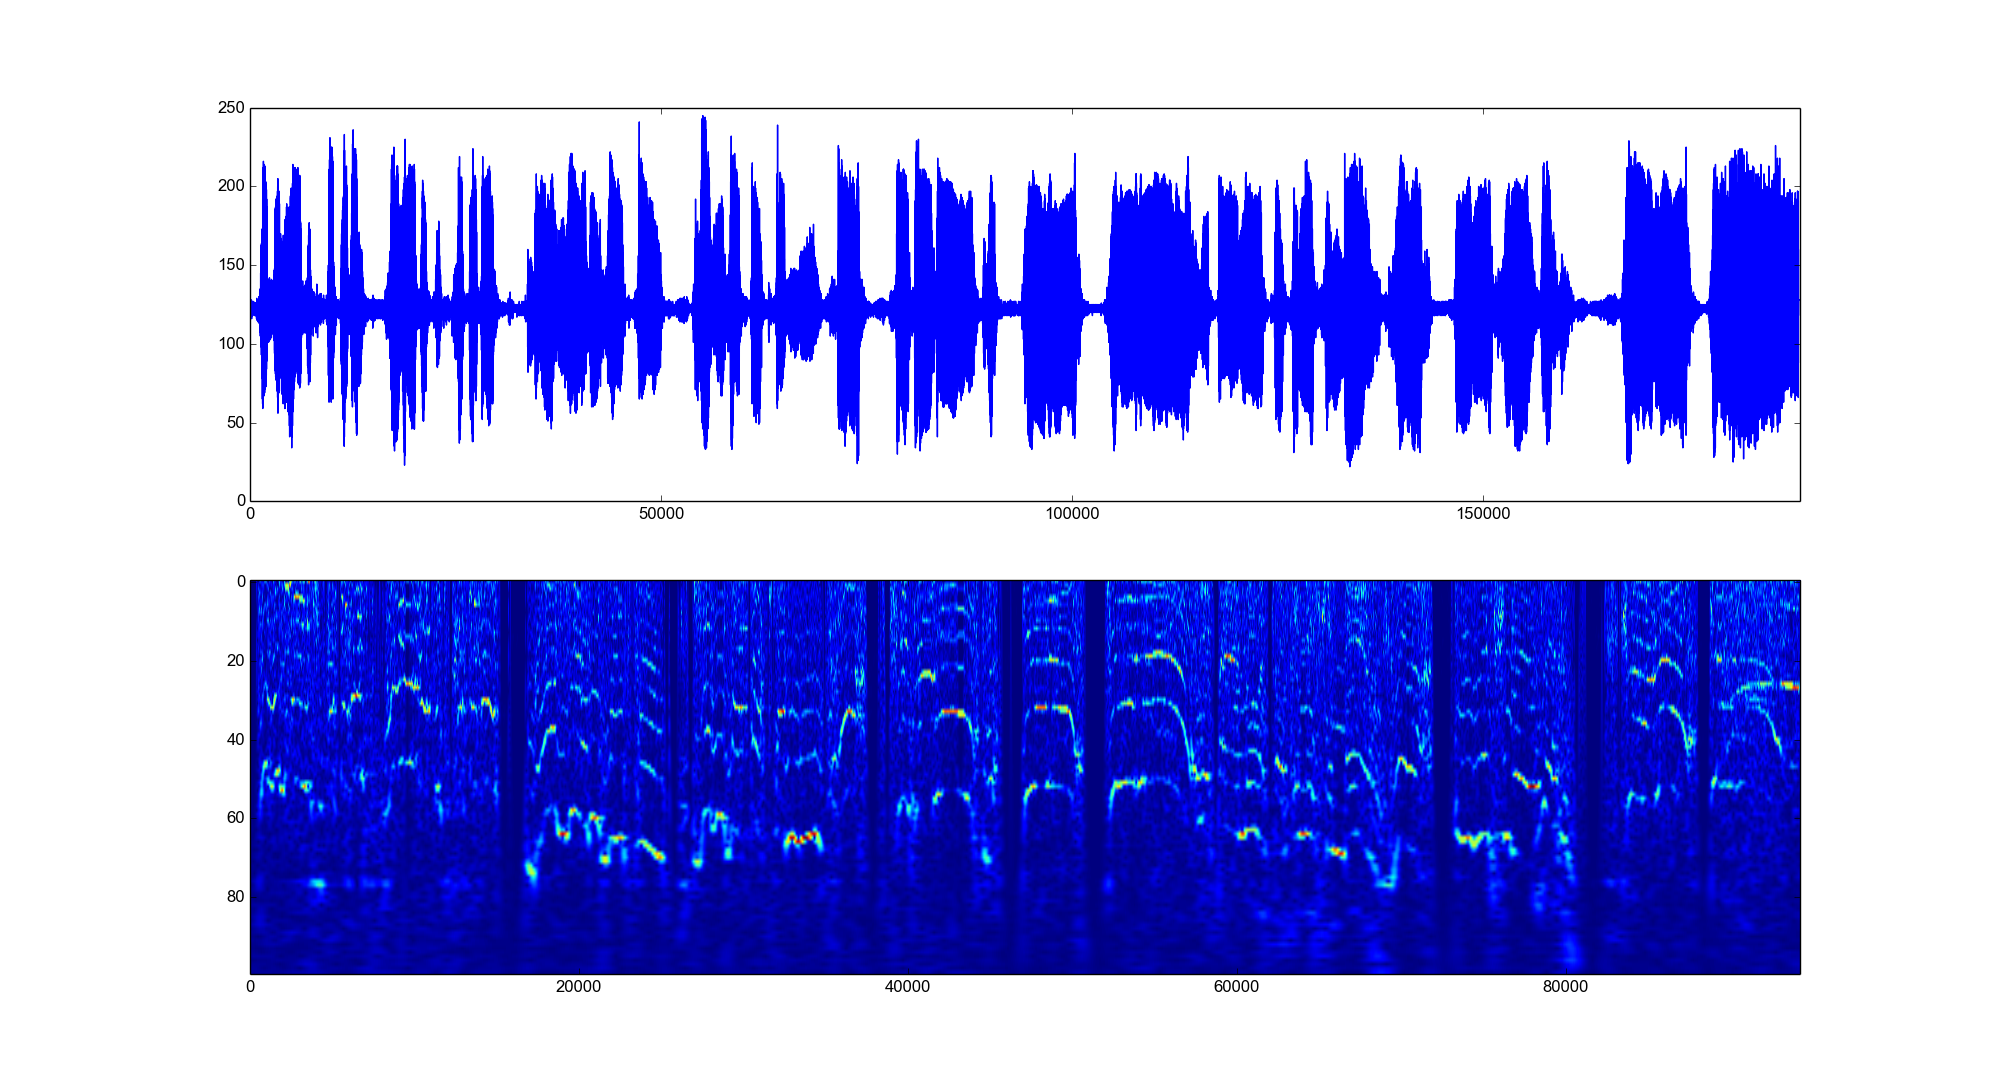
\includegraphics[scale=0.22]{figure_1.png}\\[2pt]
%
\includegraphics[scale=0.22]{couv_logo.png}}
\date{}



\begin{document}
\maketitle


\newpage

\tableofcontents
\newpage
\section{Introduction}

With the computational power available today, machine learning is becoming a very active field finding its applications in our everyday life. One of its biggest challenge is the classification task involving data representation (the preprocessing part in a machine learning algorithm). In fact, classification of linearly separable data can be easily done. The aim of the preprocessing part is to obtain well represented data by mapping raw data into a "feature space" where simple classifiers can be used efficiently.
For example, almost everything around audio/bioacoustic uses MFCC features until now.
This toolbox gives the basic tools for audio representation using the C++ programming language by providing an implementation of the Scattering Network \cite{m3} which brings a new and powerful solution for these tasks. 
The toolkit of reference in scattering analysis is SCATNET from Mallat et al. \footnote{\url{http://www.di.ens.fr/data/software/scatnet/}}. This
tool is an attempt to have some of the scatnet features more
tractable in large dataset.
Furthermore, the use of this toolbox is not limited to machine learning preprocessing. It can also be used for more advanced biological analysis such as animal communication behaviours analysis or any biological study related to signal analysis.\\
This toolbox gives out of the box executables that can be used by simple bash commands. Finally, for each presented algorithm, a graph is provided in order to summarize how the computation is done in this toolbox.\\

As we will review in the next part, we will need to perform data manipulation on huge dataset. It becomes important to have fast and efficient implementations in order to deal with this new "Big Data" era. The first descriptions concern mandatory utilities, such as audio file IO and basic tools (fft,...) that are necessary for the scattering network implementation.

\part{Fast Scattering}
\chapter{Scattering Network}


The Scattering Network aims to find a better data representation after numerous transformations of a raw input. It's been developed by St\'ephane MALLAT and its team and the only available implementation is in Matlab which provides high-level programming but is not optimal in term of execution time. 
In fact, this algorithm just started to be applied in concrete challenges and finds its limitation in the required time to complete the transformation on massive dataset. We will review its core ideas and the implementation architecture chosen in C++.

\section{Introduction}\label{conv}


The basic idea is to perform series of linear and non linear operations on a $1D$ given input signal $x$. The linear operations are done through the convolutions while the non linear ones are the use of the absolute value on these convolutions. The use of the latter allows fast convergence by the contractive property. The convolutions of the first layer $|x \star \psi_{\lambda_1}|$ are basically decomposing the signal into a wavelet basis. A parallel can be made with the FFT and the complex sine decomposition. In addition, the application of the low-pass filter $\phi$ brings time invariance (of length depending on the $\phi$ support/bandwidth).


The structure itself of the network can be compared to a Convolutionnal Neural Network where the filters are given and fully determined by the meta parameters and not learned during a training phase. This is a huge difference in term of computation time allowing good representation without training. We have to keep in mind that filters generation is also complex and time consuming.


The mapped data into the feature space can be used for simple data analysis or data learning but it finds its best use in classification. In fact, this feature space is much more suited for the use of linear classifier.
Note that in this implementation we won't look at the reconstruction problems since our main goal is not to use the Scattering Network for compression,reconstruction,...
Let's look at the general picture of the scattering network and analyse it briefly.
\\
%\begin{figure}[H]
%\begin{center}
%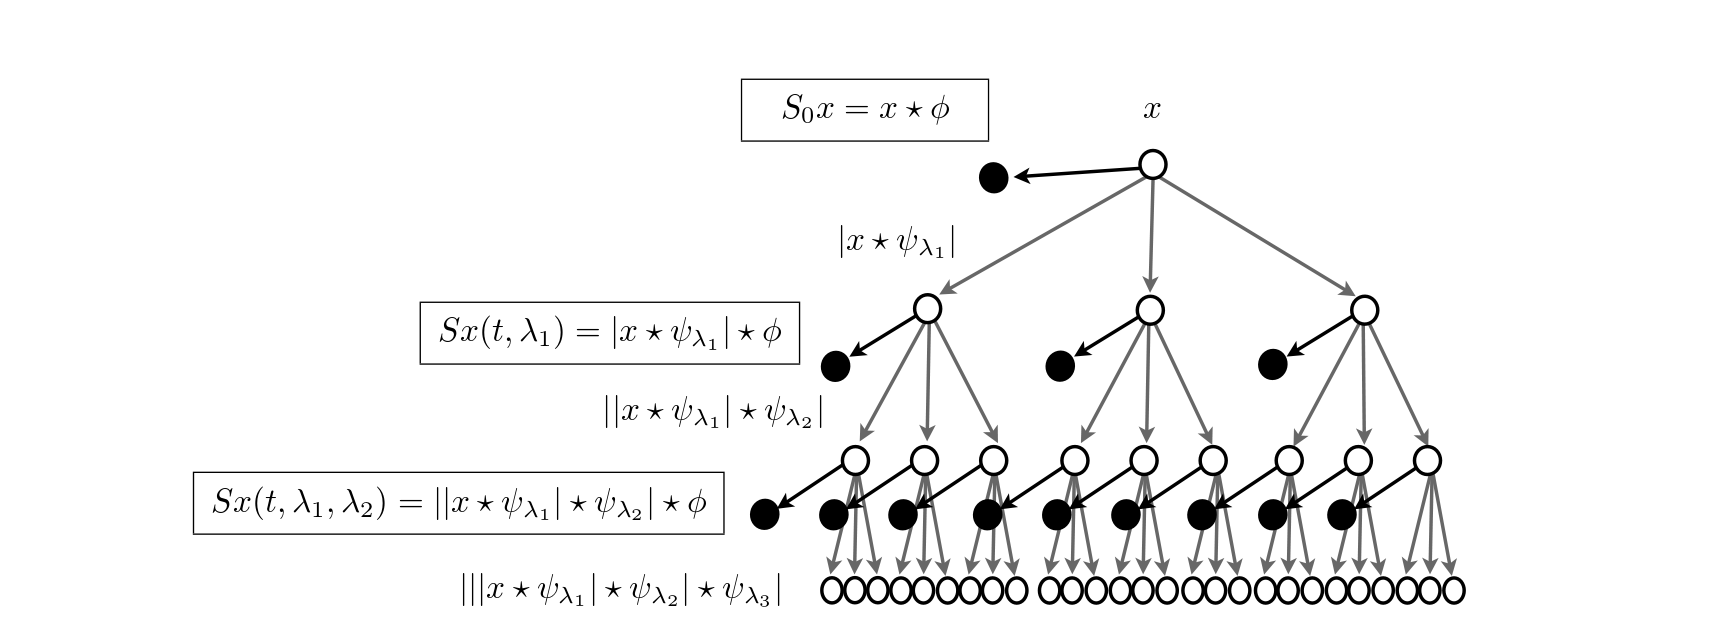
\includegraphics[scale=0.23]{scattering.png}\label{oo}\caption{Scattering Summary.\cite{m2}}
%\end{center}
%\end{figure}


In this case the scattering network is made of $3$ layers. Each layer has a specific low-pass filter ($\phi_i,i=0,1,2,3$) and high-pass filter banks ($\psi_1,\psi_2,\psi_3$). In our specific case of $1D$ signals, there is only one $\phi$ per layer. Given an input signal $x$ of size $N$ we perform a low-pass decomposition $|x \star \phi_0|:=S_0x$ and a high-decomposition $ x \star \psi_{1,\lambda_1}$. Note that the convolutions are then sub-sampled leading to a output size of $|\lambda_1| \times 2N/T$ for $U_1$. The sub-sampling only reduce coefficient redundancy and depends on the $T$ coefficients. The $i^{th}$ filter of a given high-pass filter bank is generated by the meta parameters of the corresponding layer.
\\Finally on these convolutions is applied the absolute value operation leading to the high-decomposition $U_1:=|x \star \psi_{1,\lambda_1}|$ of the first scattering layer. The scattering coefficients are then easily computed with the application of the low-pass filter $\phi_1$ leading to the scattering coefficient per say $U_1 \star \phi_1:=S_1$. 
\\
Then for the second layer, each one of the previous high-decomposition row is treated as an input signal and the same algorithm is performed again. Details about this will be given in the scattering layer section\ref{ll} but we can already note that the meta parameters are specific to each scattering layer.
Finally let's review what the meta parameters are about :
\begin{itemize}
\item $T$ determines the $\phi$ support/bandwidth, this is basically the invariant time window. Taking a great $T$ leads to huge time invariance but at the cost of variance (and information) loss with respect to the time dimension.
\item $Q$ determines the quality factor (the number of filters per octave)
\item $J$ determines the number of octave to go through.
\item $PE$ (Periodization Extent) is the constant used in the filter periodization ($1$ by default)
\end{itemize}

\section{Filter Bank}
Filters are created given the meta-parameters, the support size an the filter position in the filter bank. Using this, the coefficients $\sigma$ and $\xi$ are deduced.\\
For the $\psi$ generation, it is efficient to loop through $\gamma$ since the meta parameters and the total size of the filters are the same (only the filter number in the filter bank changes). Note that the support of these filters expands when $\lambda$ increases.
On the other hand, creating a specific filter with just the bandwidth and frequency max. position is more efficient and is thus used for the $\phi$ generation. In fact, since only one low-pass filter is made per layer, we just have to compute $\xi$ and $\sigma$ for this filter.


The filters are directly computed in the Fourier domain to speed up the decomposition algorithm, indeed we only have to compute the FFT of the input to perform the decomposition algorithm now. Here $\xi$ corresponds to the central frequency and so to the global maximum position. It can be seen as a position parameter while $\sigma$ is a scale parameter. In practice, in order to generate the filters we always take the mother coefficients that are transformed through a scaling coefficient with exponential rate. We have then as mother coefficients :
\[
\Xi=\frac{\pi}{2}*(2^{-1/Q}+1)
\]
\[
\Sigma=\sqrt{3}*(1-2^{-1/Q})
\]
The scaling factor for the filter $i$ is :$\lambda_i=2^{-i/Q}$ which leads to the following coefficients for any given filter $i$ for a specific layer having the same meta parameters :
\[
\xi_i=\Xi*\lambda_i
\]
\[
\sigma_i=\Sigma*\lambda_i
\]


\paragraph{Filters} In this implementation, high-pass filters are Morlet wavelets while low-pass filters are Gabor filters. Note that Morlet filters are actually another name for Gabor kernels. The difference between the Gabor function (non-zero-mean function) and the Gabor kernel (zero-mean function) is that the Gabor kernel satisfies the admissibility condition for wavelets (integral equals to $0$), thus being suited for multi-resolution analysis. The admissibility condition ensures that the inverse transform and Parseval formula are applicable.

\paragraph{Filter Periodization}
In order to increase resolution of the filters, we can compute them on a bigger interval than the one we are interested in and then periodize them in the Fourier domain :
\[
f(x)=\sum_{n\in \mathcal{Z}} f(x+2\pi n) 
\]
In practice nothing assures the convergence for any function $f$ but our filters are generated through Gaussian functions which actually guarantees the convergence. In practice, we use $n\in \{-PE, -PE+1,...,PE,PE+1 \}$ with $x \in \{ x \in \mathbb{R}, i=0,...,T-1 : x= i*2\pi/T\} $ which is similar to $x \in \{0,2\pi/T,2*2\pi/T,...,(T-1)2\pi/T \} $.
With this definition $x$ covers $[0,2\pi[$ with $T$ points linearly separated by a distance of $1/T$.
In all the examples presented here a periodization extent of $1$ is used.
\\
The $n$ coefficients affect the range on which the wavelet is evaluated which grows with bigger $n$ : 
\[ [  -2\pi * PE, 2\pi*(1+PE)-1/T ] \]
It is then shrunk into the desired support size by the periodization process.

\section{Scattering Layer}\label{ll}
The scattering layer performs the decomposition of the raw input given the meta parameters and the filter banks by performing the decomposition process. 
\\
With the filter bank, all the $\psi$ filters are available and we can apply Littlewood-Paley normalization necessary because of the logarithmic spaced filters.

\paragraph{Decomposition Implementation}
The core of the algorithm lies in this decomposition. Firstly, the convolution defined in the section \ref{conv} is redundant and so is only performed on every $T/2$ spaced points. This implies a reduced output length and faster computation. Thus, it is necessary to perform a periodization before computing the IFFT (allowing a time sub-sampling). The output length must then be $\text{InputSize}*2/T$. Doing this for each $\psi$ filter gives the output of the layer.
Here is a simple scheme to emphasize the algorithm :
\\
\\
\begin{algorithm}[H]
 \KwData{Input,inputN,inputM,Meta Parameters}
 \KwResult{Output,outputN,outputM}
 NumberOfPsis=J*Q\;
 outputN=inputN*NumberOfPsis\;
 outputM=inputM$*2/T$\;
 $\psi$ Filter Bank creation\;
 $\phi$ creation\;
 \For{$i=0 \rightarrow$inputN}{
 inputFFT=FFT(input[i]);))\;
 \For{$j=0 \rightarrow$ NumberOfPsis}{	HighDecomposition[i*NumberOfPsis+j]=abs(IFFT(inputFFT$.*\psi_{L,j}$)\;
 Scattering[i*NumberOfPsis+j]=IFFT(periodize( FFT(HighDecomposition[i*NumberOfPsis+j]$.*\phi_{L}$)))
  }
  }
 \caption{Decomposition Algorithm of the layer $L$}
\end{algorithm}

With "periodize" being the function that will periodize the result in order to sub-sample in the time domain to obtain the desired output size. 
For example the array $[0,1,2,3,4,5]$ is equal to $[3,5,7]$ after a periodization by a factor of $2$.


The degrees of freedom of the model are : 
\begin{itemize}
\item $T$
\item $Q$
\item $J$
\item $h_1$
\end{itemize}
Where we have :\\ 
\[
U_1=\left( \begin{matrix}
|x\star \psi_{1,1} | \\
|x\star \psi_{1,2} | \\
... \\
|x\star \psi_{1,|\lambda_1|} |\\
\end{matrix}
\right)
\in \mathbb{R}^{|\lambda_1|\times N_1}
\]

\[
S_1=\left( \begin{matrix}
|x\star \psi_{1,1} | \star \phi_1 \\
|x\star \psi_{1,2} | \star \phi_1  \\
... \\
|x\star \psi_{1,|\lambda_1|} | \star \phi_1 \\
\end{matrix}
\right)
\in \mathbb{R}^{|\lambda_1|\times N_2}
\]

\[
U_2=\left( \begin{matrix}
||x\star \psi_{1,1} | \star \psi_{2,1} |\\
||x\star \psi_{1,2} | \star \psi_{2,1} |\\
... \\
||x\star \psi_{1,|\lambda_1|} |\star \psi_{2,1}|\\
||x\star \psi_{1,1} | \star \psi_{2,2} |\\
||x\star \psi_{1,2} | \star \psi_{2,2} |\\
... \\
||x\star \psi_{1,|\lambda_1|} |\star \psi_{2,2}|\\
...\\
||x\star \psi_{1,1} | \star \psi_{2,| \lambda_2|} |\\
||x\star \psi_{1,2} | \star \psi_{2,| \lambda_2|} |\\
... \\
||x\star \psi_{1,|\lambda_1|} |\star \psi_{2,| \lambda_2|}|
\end{matrix}
\right)
\in \mathbb{R}^{|\lambda_1|* | \lambda_2 |\times N_3}
\]

\[
S_2=\left( \begin{matrix}
||x\star \psi_{1,1} | \star \psi_{2,1} |\star \phi_2 \\
||x\star \psi_{1,2} | \star \psi_{2,1} |\star\phi_2 \\
... \\
||x\star \psi_{1,|\lambda_1|} |\star \psi_{2,1}|\star\phi_2 \\
||x\star \psi_{1,1} | \star \psi_{2,2} |\star\phi_2 \\
||x\star \psi_{1,2} | \star \psi_{2,2} |\star\phi_2 \\
... \\
||x\star \psi_{1,|\lambda_1|} |\star \psi_{2,2}|\star\phi_2 \\
...\\
||x\star \psi_{1,1} | \star \psi_{2,| \lambda_2|} |\star\phi_2 \\
||x\star \psi_{1,2} | \star \psi_{2,| \lambda_2|} |\star\phi_2 \\
... \\
||x\star \psi_{1,|\lambda_1|} |\star \psi_{2,| \lambda_2|}|\star\phi_2 
\end{matrix}
\right)
\in \mathbb{R}^{|\lambda_1|* | \lambda_2 |\times N_4}
\]

\chapter{Choice for Fast Audio File Manipulation}

\section{File Structure}
The WAV file is an instance of a Resource Interchange File Format (RIFF) defined by IBM and Microsoft. The header part of this file is made of complementary chunks describing the architecture of the wav allowing easy information storing.
Let's see how these chunks are organized in a WAV file :

\begin{figure}[H]
\begin{center}
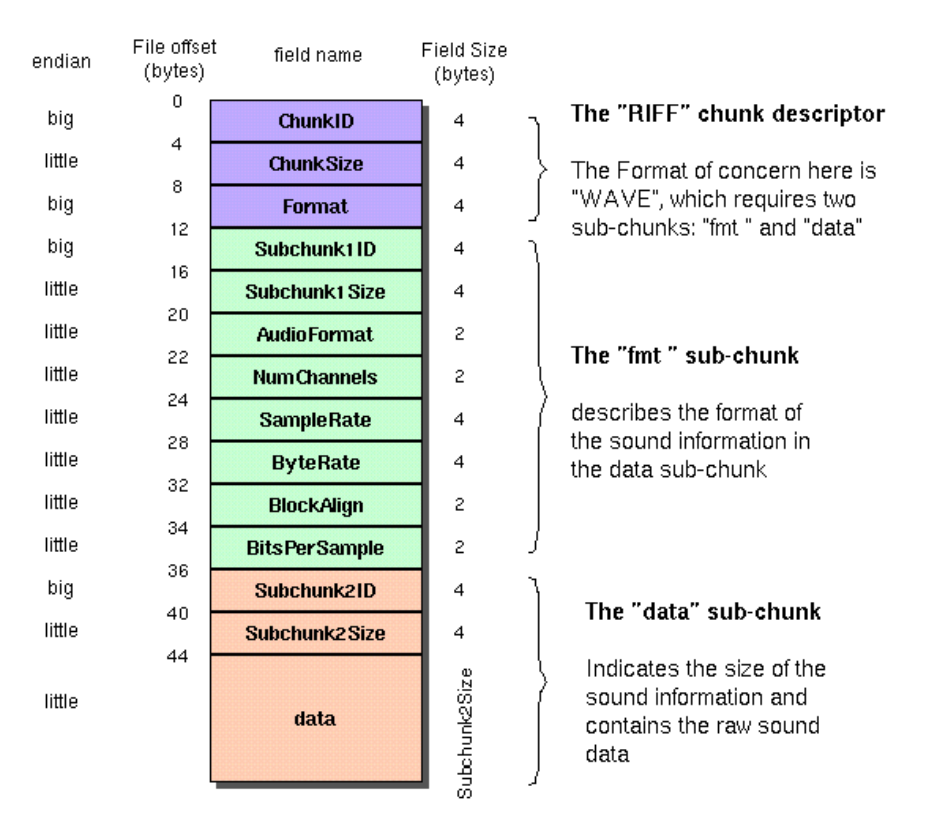
\includegraphics[scale=0.31]{wavformat.png}\caption{The Canonical WAV file format \url{https://ccrma.stanford.edu/
courses/422/projects/WaveFormat/}}
\end{center}
\end{figure}

The file is made of three main chunks each having a specific role that we will describe here.
\subsection*{Chunk}
\begin{itemize}

\item ChunkID identifies the type of the first chunk with four characters : "RIFF".
\item ChunkSize is the size of the file left from this point. It will be 36 (sum of the other chunks sizes) plus Subchunk2Size and this can be easily seen by summing the different sizes on the right of the header representation.
\item Format will be four characters : "WAVE" (this allows us to check if we are really reading a wav file during the process).
\end{itemize}

\subsection*{Sub Chunk 1}
\begin{itemize}
\item SubChunk1ID identifies the second chunk. It is a four characters name : "fmt "  and starts the data description block. 
\item SubChunk1Size is simply the size of this block which is 16. 
\item AudioFormat, also called Format tag, is the option indicating the data compression used. It is almost always equal to $1$ which stands for : no compression is used. 
\item NumChannels is the number of channels ($1$ for mono and $2$ for stereo). 
\item SampleRate is simply the number of samples per second, the frequency. 
\item ByteRate is the average number of bytes per second, this can be found with the following formula : $\text{SampleRate} * \text{NumChannels}*\frac{\text{BitsPerSample}}{8}$. 
\item BlockAlign won't be necessary for us. It can be computed with the formula : $NumChannels*\frac{\text{BitsPerSample}}{8}$.
\item BitsPerSample can either be $8$ or $16$ but in general the later is used.
\end{itemize}

\subsection*{Sub Chunk 2}
\begin{itemize}
\item SubChunk2ID identifies the last chunk block, it is made of the four characters : "data".
\item Subchunk2Size is the size of the file left which is just the size of the data. 
\item Data is the block containing the values of the signal in the standard pulse-code modulation representation.
\end{itemize}


\section{Implementation}
The use of the built-in class WAV is simple, the only thing to provide is the name of the wav file. This can be done during the instantiation of the class or at any other time. Let's look at an example.
\begin{lstlisting}[basicstyle=\tiny]
    WAV<double> Signal("mysignal.wav");
    WAV<double> Signal2;
    "mysignal.wav">>Signal2;
    "mysignal2.wav">>Signal;
\end{lstlisting}
The template parameter can be ignored leading to the default value : float. One instance of the class can be used for different wav files which can be useful. This WAV variable allows easy interactions and can provide informations about the loaded file :

\begin{lstlisting}[basicstyle=\tiny]
    Signal._Size;
    Signal._SampleRate;
    Signal_NumberOfChannel;
    Signal[i];//return the ith value of the loaded signal
\end{lstlisting}
Finally, to export the loaded file two options are available. Firstly, it is possible to export it into a .txt file which only exports the signal data disregarding all the other informations. This loss can be avoided using a special method which exports the data back into a wav file, with the following syntax :

\begin{lstlisting}[basicstyle=\tiny]
    Signal>>"newsignal.txt";//to .txt
    Signal.PrintWav("newsignal.wav");//to .wav
\end{lstlisting}
With this implementation, WAV can be seen as a special type. Note that no normalization is used. In fact, only the user can define the normalizing constant he is interested in (max, $L^2$-norm,...) and so has to apply it after the import.
Finally, for an external use of this toolbox, one should not need to use this class since it is just here as a input/output convenience for the other algorithm we will now describe.

\chapter{Fast Fourier Transform implementation}
\section{Definitions}
A sinusoidal wave is characterised by three parameters: amplitude, frequency and phase.
\begin{itemize}
\item The amplitude is the amount the function varies, positively or negatively, from zero in the y direction.
\item The frequency is how many complete cycles there are of the wave in unit distance on the x axis (which often measures time).
\item The phase is relevant when comparing two waves of the same frequency. It is how much (measured in degrees or radians) one is shifted relative to the other on the x axis.
\end{itemize}
This terminology comes from sound engineering where higher frequency sounds have higher pitch and waves of greater amplitude are louder.
As an alternative of specifying the frequency, the number of cycles in unit distance, we can instead specify the wavelength : the length of one cycle. The higher the frequency, the shorter the wavelength. The lower the frequency the longer the wavelength.
\\
The Nyquist frequency is the maximum frequency that can be detected for a given sampling rate and it is half of this sampling rate. This is because in order to measure a wave one needs at least two sample points to identify it (trough and peak).
We will abbreviate the continuous Fourier transform with CFT and the discrete Fourier transform with DFT.
\paragraph{Interpretation of the CFT}
Using the Euler's formula, we can see the Fourier Transform as a decomposition of a signal into complex sinus by the use of convolutions.
\[
e^{ix}=\cos(x)+i\sin(x)
\]
\begin{align*}
\hat{f}(\xi)&=\int_{-\infty}^{\infty} f(x) e^{-2\pi i x \xi}dx\\
&=\int_{-\infty}^{\infty} f(x) (\cos(-2\pi x \xi)+i\sin(-2\pi x \xi))dx\\
&=\int_{-\infty}^{\infty} f(x) \cos(-2\pi x \xi)+f(x)i\sin(-2\pi x \xi)dx\\
&=\int_{-\infty}^{\infty} f(x) \cos(-2\pi x \xi) dx + \int_{-\infty}^{\infty} f(x)i\sin(-2\pi x \xi)dx
\end{align*}

\section{Fast Fourier Transform}
We will now denote $x_k$ as the $k^{th}$ value on the signal in the time space and $X_k$ the $k^{th}$ value of the signal in the frequency domain, $N$ will denote the length of the signal. A length of $N$ means the indices range from $0$ to $N-1$.
\\
The fast Fourier transform (FFT) is a instance of DFT which is able to perform the DFT in $O(N\log(N))$ complexity.\\
The DFT formula using the Twiddle Factor notation :
\begin{align*}
\forall k \in \mathbb{Z},&X_k=\sum_{n=0}^{N-1} x_n e^{\frac{-2\pi i k n}{N}}\\
&X_k=\sum_{n=0}^{N-1} x_n W_N^{kn}
\end{align*}
As we can see, we need to perform $N$ operations for each $X_k,k\in \{0,1,...,N-1\}$ thus we are in $O(N^2)$ complexity.
\\
Note that it is possible to use the scaling factor :$1/\sqrt{N}$ in order to have an unitary operator (Parseval's theorem) which implies that the sum (or integral) of the square of the function is equal to the sum (or integral) of the square of its transform which is not needed in this toolbox thus not used.\\
In order to go from $N^2$ operations to $N\log(N)$ operations, three main concepts have to be defined :
\begin{itemize}
\item The Danielson-Lanczos Lemma
\item The Twiddle Factor properties
\item The Butterfly Scheme
\end{itemize}

\paragraph{Danielson-Lanczos Lemma}
This theorem is the foundation of the FFT by allowing a divide and conquer strategy. In fact, we have the following relations :
\begin{align*}
X_k=&\sum_{n=0}^{N-1} x_n e^{\frac{-i2 \pi k n}{N}}\\
=&\sum_{n=0}^{\frac{N}{2}-1} x_{2n} e^{\frac{-i2 \pi 2k n}{N}}+ x_{2n+1} e^{\frac{-i2 \pi (2k+1) n}{N}}\\
=&\sum_{n=0}^{\frac{N}{2}-1} x_{2n} e^{\frac{-i2 \pi k n}{N/2}}+\sum_{n=0}^{\frac{N}{2}-1}x_{2n+1} e^{\frac{-i2 \pi 2k n-i2 \pi n}{N}}\\
=&\sum_{n=0}^{\frac{N}{2}-1}x_{2n} e^{\frac{-i2\pi k n}{N/2}}+W_N^k\sum_{n=0}^{\frac{N}{2}-1}x_{2n+1} e^{\frac{-i 2 \pi k n}{N/2}}
\end{align*}
For every $X_i$ we can now divide the $N$ sums into two different summation group (Even and Odd). Note that for the special case $N=2$ the sums are removed and n is replaced by $0$ which means that we are left with a simple linear combination of the input signal and the Twiddle Factor. 
If we apply this recursively we obtain the following architecture :


And now for any given input size we are able to break it done into a linear combination of the input signal with twiddle factors.
For example, if $N=4$ we have after full decomposition :
\[
X_k=x_0+W_2^kx_2+W_4^kx_2+W_4^kW_2^kx_3
\]
And for $N=8$ :
\[
X_k=x_0+W_2^kx_4+W^k_4x_2+W_4^kW_2^kx_6+W_8^kx_1+
W_8^kW_2^kx_5+W_8^kW_4^kx_3+W_8^kW_4^kW^k_2x_7
\]
This puts a constraint though, the signal length has to be a power of $2$. The number of decomposition is thus $\log_2 (N)$.
If the signal size is not a power of $2$ it is necessary to use zero padding (add as may $0$ as necessary at the end of the input). Padding with $0$ in time domain leads to an interpolation of the FFT. Middle zero padding the FFT (in the frequency domain) interpolates the IFFT (time domain). Periodizing in the frequency domain implies sub-sampling in the time domain (this will be useful for the Scattering Network).
\\
One last thing to notice here is the order of the input values in the decomposition. Because of the nature of this decomposition (even/odd) we end up with the $x$ terms being rearranged in a specific order : the bit-reversal order. This can be found by taking the symmetric of the binary position of the input value as seen in this little example for $N=8$:
\begin{align*}
0:000\rightarrow000:0\\
1:001\rightarrow100:4\\
2:010\rightarrow010:2\\
3:011\rightarrow110:6\\
4:100\rightarrow001:1\\
5:101\rightarrow101:5\\
6:110\rightarrow011:3\\
7:111\rightarrow111:7\\
\end{align*}

\paragraph{Twiddle Factor Properties}
Complexity has already been broken down but we can still optimize the implementation by exploiting the Twiddle Factor properties using roots of unity properties. In fact we have :
\[
W_N^k=e^{\frac{-i 2 \pi k}{N}}=\cos(2\pi k/N)-i\sin(2 \pi k/N)
\]
Thus for $N=2$:
\begin{align*}
&W^0_2=W^2_2=W_2^4=...\\
&W_2^1=W_2^3=W_2^5=...
\end{align*}
\\And for $N=4$
\begin{align*}
&W_4^0=W_4^4=W_4^8=...\\
&W_4^1=W_4^5=W_4^9=...\\
&W_4^2=W_4^6=W_4^{10}=...\\
&W_4^3=W_4^7=W_4^{11}=...
\end{align*}
And so on using trigonometric properties, with functions here being $N\pi$-periodic.
So using this will allow us to perform less Twiddle Factor computation at each level.
\paragraph{Butterfly Scheme}
Finally, the last brick is the butterfly scheme that can be seen in the next diagram\ref{bb} allowing an in-place FFT which is memory friendly.

\section{Inverse Fourier Transform}
In order to simplify the algorithm we sill use the following formula :
\[
IFFT(x)=\frac{1}{N}conj(FFT(conj(x)))
\]
\section{Algorithm}
Firstly, our implementation is made of three nested loops, the main one which will go through the $\log(N)$ levels of decomposition. The second one will go through the blocks inside a specific level (the last level as $1$ block whereas the first level as $N/2$ blocks). Finally the last loop will go inside a block (a block on the first decomposition level will have size $2$ while the block in the last decomposition level will be of size $N$). For each level ($i$), only $2^i$ Twiddle factors are computed in the main loop where $i$ is the decomposition level from $0$ to $\log(N)-1$. A simple temporary variable is used in order to perform the swapping operations. Here is an instance of this implementation for $N=8$ and a human friendly output explaining the performed steps.
\begin{figure}[H]
\begin{center}
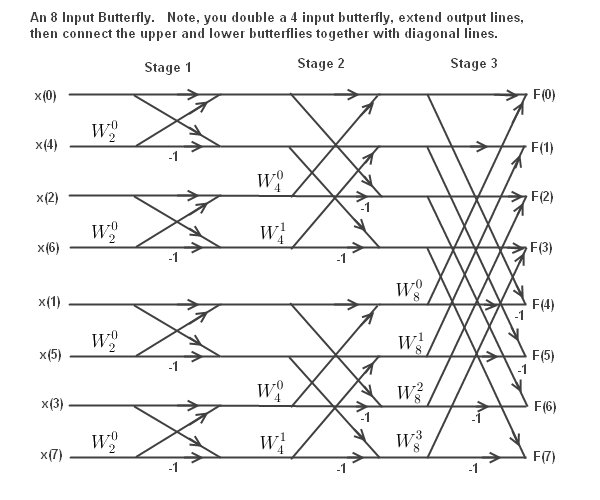
\includegraphics[scale=0.7]{Butterfly8.jpg}\label{bb}
\caption{Full FFT computation with $N=8$ \cite{learnfft}}
\end{center}
\end{figure}
This simple example performs the following computation in the implemented algorithm :

\begin{lstlisting}[basicstyle=\tiny,caption=Computation done during the FFT computation of a signal of size $8$. Each column represents the overall loop 9$log(N)$ iterations. $W$ is the Twiddle Factor and each block is the inner loop performing the butterfly scheme.]

Level : 0
   W[0]=W(0,2)
   Block : 0
     signal[1]*=W[0]
     tmp=signal[0]
     signal[0]+=signal[1]
     signal[1]=tmp-signal[1]

   Block :  1
     signal[3]*=W[0]
     tmp=signal[2]
     signal[2]+=signal[3]
     signal[3]=tmp-signal[3]

   Block :  2
     signal[5]*=W[0]
     tmp=signal[4]
     signal[4]+=signal[5]
     signal[5]=tmp-signal[5]

   Block :  3
     signal[7]*=W[0]
     tmp=signal[6]
     signal[6]+=signal[7]
     signal[7]=tmp-signal[7]
Level :  1
   W[0]=W(0,4),W[1]=W(1,4)
   Block :  0
     signal[2]*=W[0]
     tmp=signal[0]
     signal[0]+=signal[2]
     signal[2]=tmp-signal[2]
     signal[3]*=W[1]
     tmp=signal[1]
     signal[1]+=signal[3]
     signal[3]=tmp-signal[3]

   Block :  1
     signal[6]*=W[0]
     tmp=signal[4]
     signal[4]+=signal[6]
     signal[6]=tmp-signal[6]
     signal[7]*=W[1]
     tmp=signal[5]
     signal[5]+=signal[7]
     signal[7]=tmp-signal[7]
Level :  2
   W[0]=W(0,8),W[1]=W(1,8)
   W[2]=W(2,8),W[3]=W(3,8)
   Block :  0
     signal[4]*=W[0]
     tmp=signal[ 0 ]
     signal[0]+=signal[4]
     signal[4]=tmp-signal[4]
     signal[5]*=W[1]
     tmp=signal[1]
     signal[1]+=signal[5]
     signal[5]=tmp-signal[5]
     signal[6]*=W[2]
     tmp=signal[2]
     signal[2]+=signal[6]
     signal[6]=tmp-signal[6]
     signal[7]*=W[3]
     tmp=signal[3]
     signal[3]+=signal[7]
     signal[7]=tmp-signal[7]
\end{lstlisting}

The Twiddle Factors are computed at the start of each main loop computing the needed values which are then reused throughout the blocks, meaning that for the first level only one value is computed and then reused all along the blocks.
Here is an example of the use :

\begin{lstlisting}[basicstyle=\tiny]
    WAV<> wav("signal.wav");//load a wav into float type array
    fft<> signalfft(signal.ptr(),signal._Size);//default padding option=1
    signalfft.ComputeFFT();
    signalfft.ComputeIFFT();//get back to the original signal
    signalfft[2];//access the second coefficient
    signalfft>>"signalfft.txt";//export it
    wav<<"processed.wav";//load a new wav
    signalfft.ComputeFFT(wav.ptr(),wav._Size);//perform a new FFT
\end{lstlisting}
Note that the parameters of the fft class are by default float and float, the first one stands for the type of the input signal and the latter for the coefficients type (complex$<$float$>$). Finally the padding option which by default is $1$ can be set to $0$ if the user is sure that the given signal is already a power of $2$, this force to skip the padding part resulting in faster computation. Also the coefficients are stored as complex type even after having performed an IFFT meaning that one needs to use a typecast to retrieve the original float type signal for example.


\section{Graph}
\begin{figure}[H]
\begin{center}
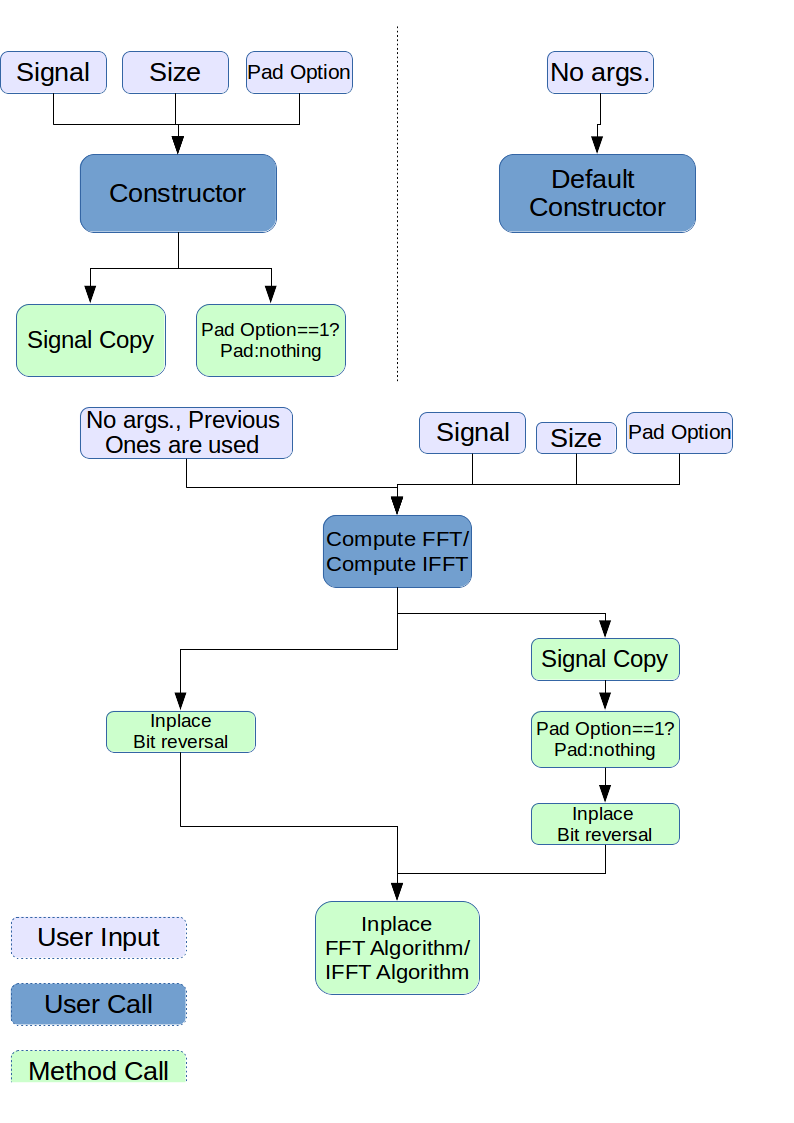
\includegraphics[scale=0.31]{fft_diagram.png}\caption{FFT Summary Diagram}
\end{center}
\end{figure}

\chapter{Spectrogram}
Each $X_k$ is a complex number that encodes how strongly the oscillation at this frequency is represented in the data but by doing an FFT we loose the time component. A useful tool is the spectrogram allowing to retrieve part of the time information. The main idea is to perform multiples FFT on a signal each one being located enough in time so the frequency information gained by the FFT can also be linked to a more or less specific time position in the signal. Note however that precision in both time and frequency is impossible to get but depending on the needs one can choose which one to enhance by modifying the size of the considered window. Larger window gives better frequency resolution but lesser time precision and vice-versa. It is easy to picture the fact that smaller windows are better for the high frequency part allowing good time precision while for low frequency a larger window has to be used for being able to capture it. This problem is lessen in wavelet decomposition and thus the scattering network since this window size is not constant any more.
\section{Algorithm}
Conceptually a spectrogram is computed with the following scheme : 
\begin{itemize}
\item splitting the signal into overlapping (or not) parts of equal length defined by the user.
\item applying to each of these chunk a windowing function (typically hanning or hamming) in order to remove artefacts by periodizing the function so the limit points (start and end of the chunk) are equal. This part is called apodization
\item computing the FFT on each of these chunks
\item for each computed FFT, taking the absolute value of the coefficients will give the columns of the spectrogram.

\end{itemize}
The windowing is needed since the FFT computation presumes that the input data repeats over and over. This is important when the initial and final values of the data are not the same because the discontinuity causes artefacts in the spectrum computed by the FFT.
\\
In addition, in this toolbox, only the first half of the FFT coefficient are put into the spectrogram thus avoiding symmetrical redundancy. This is due to the fact that our input signal is real and so the second half of the FFT coefficients is simply the complex conjugate of the first half, since in the spectrogram we display the absolute value of the coefficients, we get symmetry about the middle point.
\\ 
Most window functions afford more influence to the data at the center of the window than to the data at the edges, which represents a loss of information. To mitigate that loss, it is common to use overlapping in time (usually $50\%$).
\section{Implementation}
It is important to note that the spectrogram ($2D$-matrix) is stored by column and not by line for faster computation. In fact, during the spectrogram calculation we need to access this matrix column-wise. The operator [] returns the column while the operator () takes two arguments and return the corresponding value in a normal way. Let's look at an example :

\begin{lstlisting}[basicstyle=\tiny]
    spectrogram<> b("signal1.wav",256,0.25);//default window function : hamming
    WAV<> wav("signal2.wav");//load another wav
    b.Perform(wav.ptr(),wav._Size);//compute spectrogram given these new entries
        //and default parameters with the already declared spectrogram variable
    b>>"lifespectro.txt";//write the matrix into a txt file
    b[1][0];//second column,first element
    b(0,1);//first line second element same result as above
\end{lstlisting}

The template parameter defines the coefficients type. The default value is float. Also note that no transformation is performed after the absolute value is computed, which means that if one want to apply a logarithmic function (most common one) this has to be done after computation. 
\\
The apodization can be done using one of the available windowing function : 
\begin{itemize}
\item Hamming
\item Hanning
\item triangular
\item Hann Poisson
\end{itemize}
but can also be used with a specific user defined function passed as last argument when calling the Perfom method.
\section{Graph}
The spectrogram graph is simple and emphasizes the default parameters of the class/methods.
%\begin{figure}[H]
%\begin{center}
%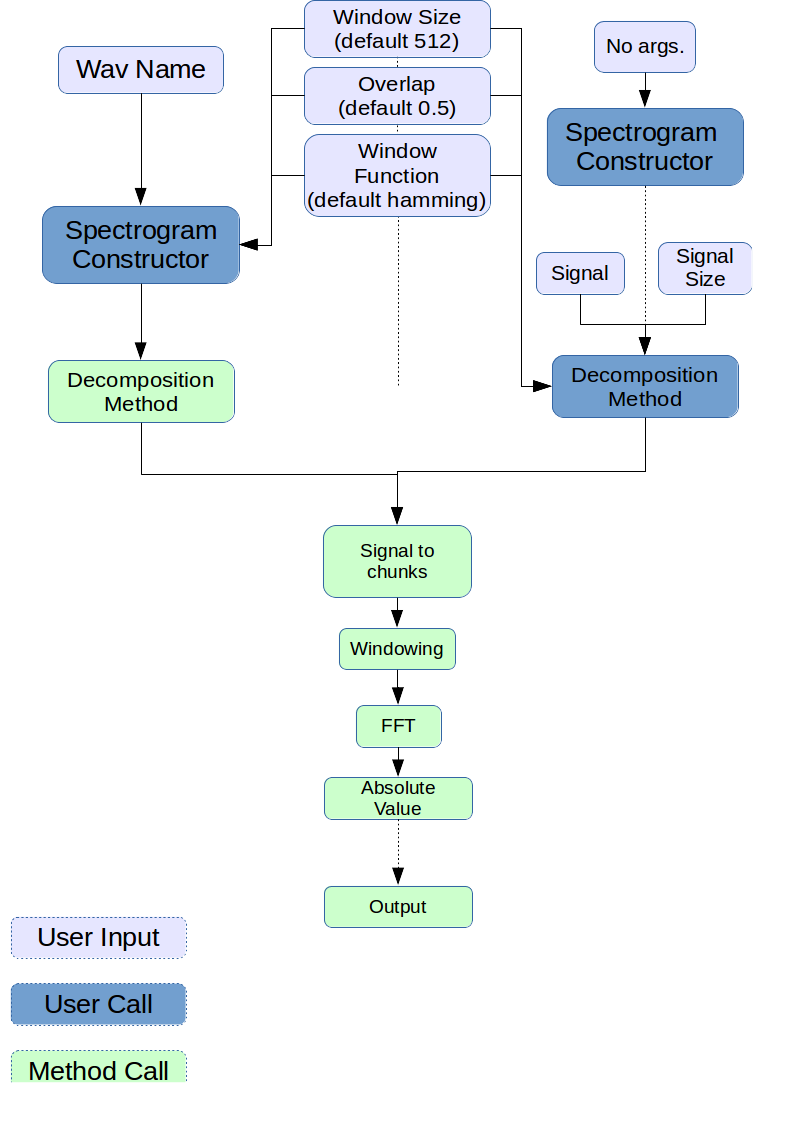
\includegraphics[scale=0.31]{spectro_diagram.png}\caption{Spectrogram Summary Diagram}
%\end{center}
%\end{figure}
\section{Examples}
Let's look at some spectrogram examples. Note that a logarithmic function has been applied to the computed values (improving coefficient representation for us).
The signals are from a bird of the BIRDLIFE CLEF Challenge 2014 \footnote{\url{http://www.imageclef.org/lifeclef/2015}}.
 and a Inia dolphin.
%\begin{figure}[H]
%\begin{center}
%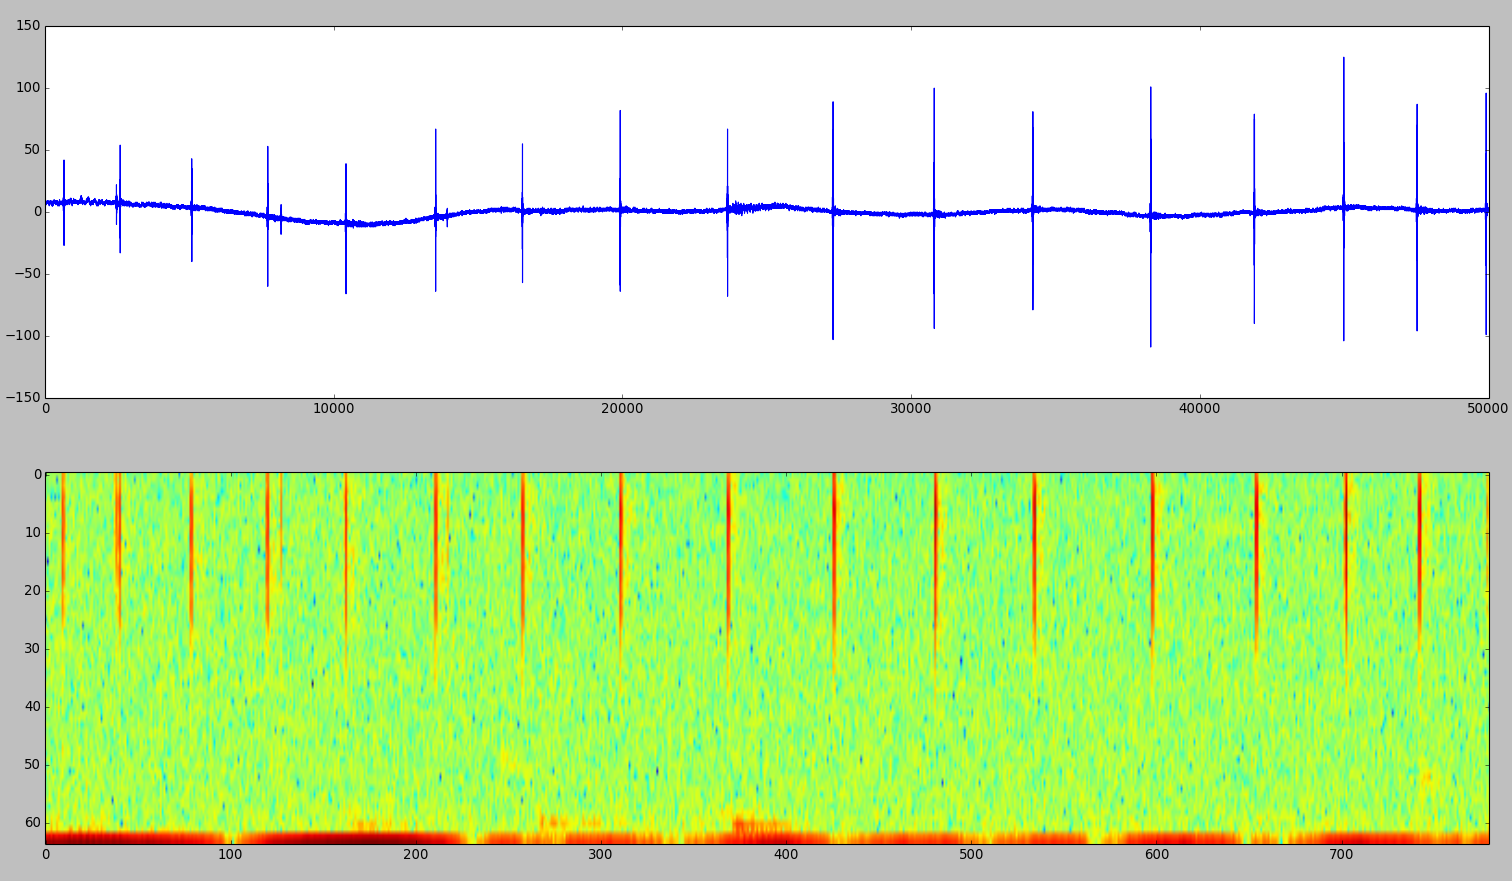
\includegraphics[scale=0.21]{fftslow.png}\caption{Inia Dolphin Slow Clicks : Spectrogram 128 50\%}
%\end{center}
%\end{figure}

%\begin{figure}[H]
%\begin{center}
%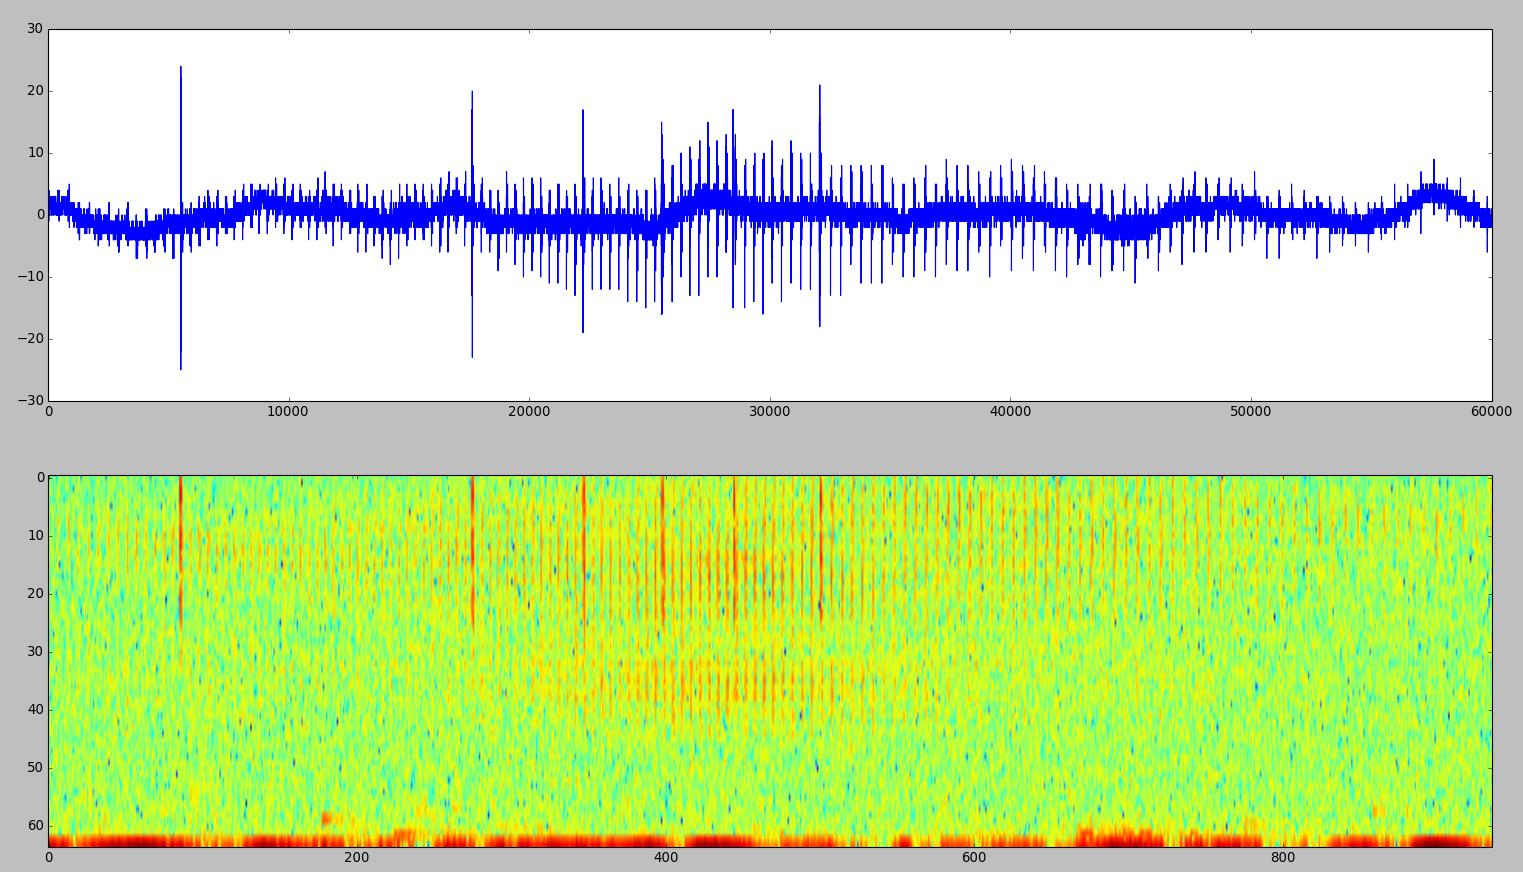
\includegraphics[scale=0.21]{fftfast.png}\caption{Inia Dolphin Fast Clicks : Spectrogram 128 50\%}
%\end{center}
\%end{figure}

%\begin{figure}[H]
%\begin{center}
%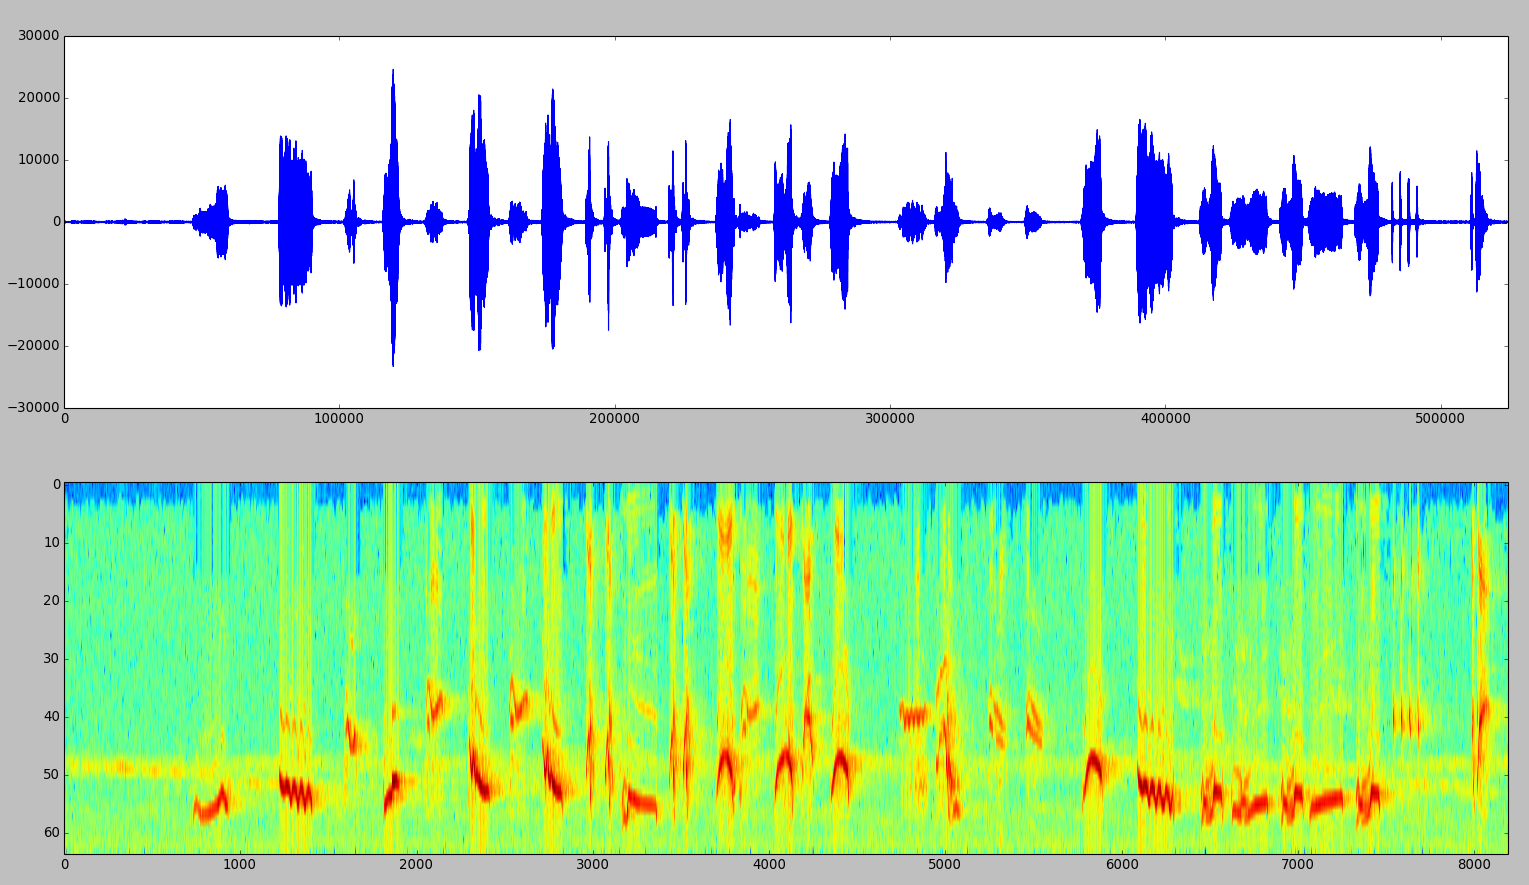
\includegraphics[scale=0.21]{fftbird.png}\caption{Bird : Spectrogram 512, 50\% }
%\end{center}
%\end{figure}


\chapter{Scattering Network Fast Implementation}
\section{Meta-Parameters}
In order to respect the scattering network architecture, this toolbox uses a specific structure : MetaParam using default parameters and a TtoJ method :

\begin{lstlisting}
   MetaParam L1param(500);
   //L1param._T=500, L1param._Q=1, L1param._J=8, L1param._PE=1
   L1param=MetaParam(500,2);
   //L1param._T=500, L1param._Q=2, L1param._J=6, L1param._PE=1
   L1param=MetaParam(500,2,4);
   //L1param._T=500, L1param._Q=2, L1param._J=4, L1param._PE=1
   L1param=MetaParam(500,4,4,4);
   //L1param._T=500, L1param._Q=4, L1param._J=4, L1param._PE=4
\end{lstlisting}

Let's now see the details of each implementation level and emphasize the implementation architecture used.
\section{Filter Bank Creation}
Filters are created through the constructor of the Filter1D class. Given meta-parameters and a support size, the constructor will initialize all the wanted variables and compute the actual filters. Note that the Filter1D class has two children : the MorletFilter1D and GaborFilter1D. These two specializations have their own filter generation algorithm. This also means that if one wants to implement a new filter, the only thing to do is to create another class of the name of this filter, inherit from the Filter1D class and implement the coefficients generation method.
\\Note that the constructor can be used in two different ways :
\begin{itemize}
\item Giving support size, meta parameters, and the position of the filter in this configuration ($gamma$)
\item Giving a support size, a $\sigma$ and a $\xi$.
\end{itemize}
The first is used to generated the $\psi$ filter bank and the second one for the $\phi$ filter.
\\
Here is an example with arbitrary coefficients :
\begin{lstlisting}
    Filter1D* BankFilter=new Filter1D[5];
    BankFilter[0]=GaborFilter1D(500,0,1,2);//500 points, xi=0,sigma=1,PE=2
    for(int i=1;i<5;++i)
        BankFilter[i]=MorletFilter1D(500,2+0.5*i,0.2*i);//500 points,xi=f(i),
                                                        //sigma=g(i),PE=1 (default)
    ofstream file("filters.txt");
    for(int i=0;i<5;++i){
        file<<BankFilter[i];// use of the overloaded operator
        file<<"\n";
    }
    delete[] BankFilter;
    file.close();

\end{lstlisting}
Giving the following result :
%\begin{figure}[H]
%\begin{center}
%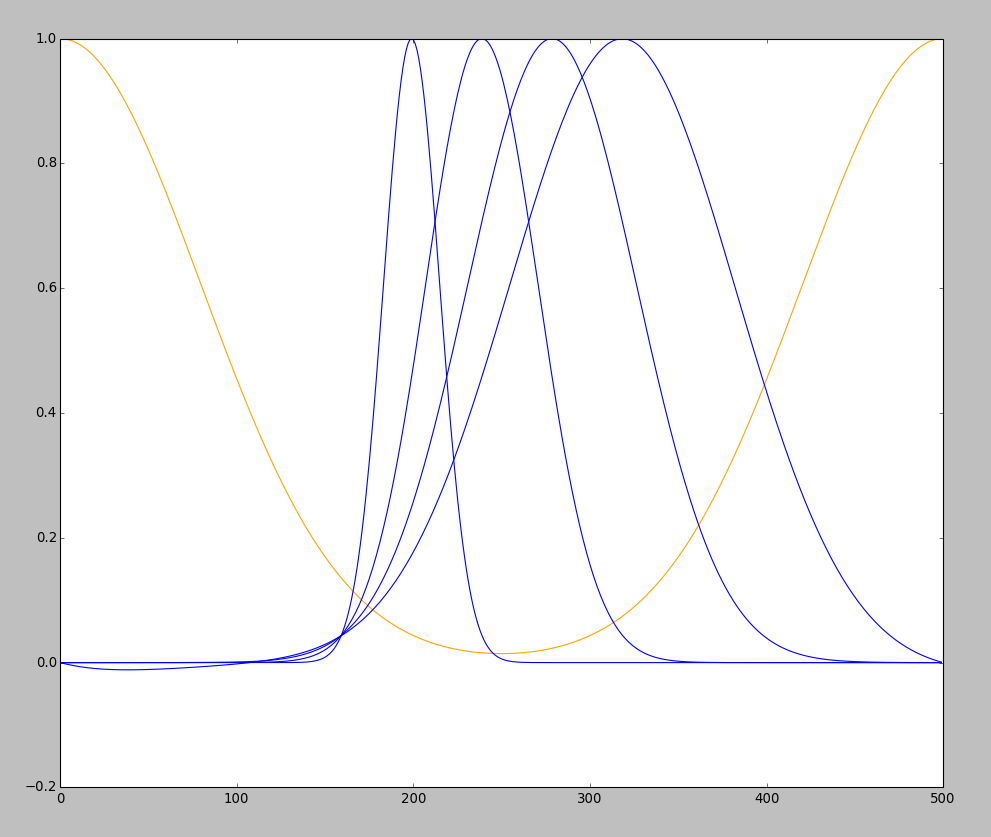
\includegraphics[scale=0.21]{example1.png}\caption{Filters generation example in the frequency domain, orange : Gabor filter, blue : Morlet wavelets.}
%\end{center}
%\end{figure}
Let's now look at the high-pass filter bank generated through a scattering layer :

\begin{lstlisting}
    
    MetaParam AA;
    AA._Q=8;
    AA._J=5;
    AA._T=4;
    ScatteringLayer LL;
    LL.CreatePsis(pow(2,10),AA);
    ofstream F("psis.txt");
    F<<LL._Psis;
    F.close();

\end{lstlisting}
Giving the following result :
\begin{figure}[H]
\begin{center}
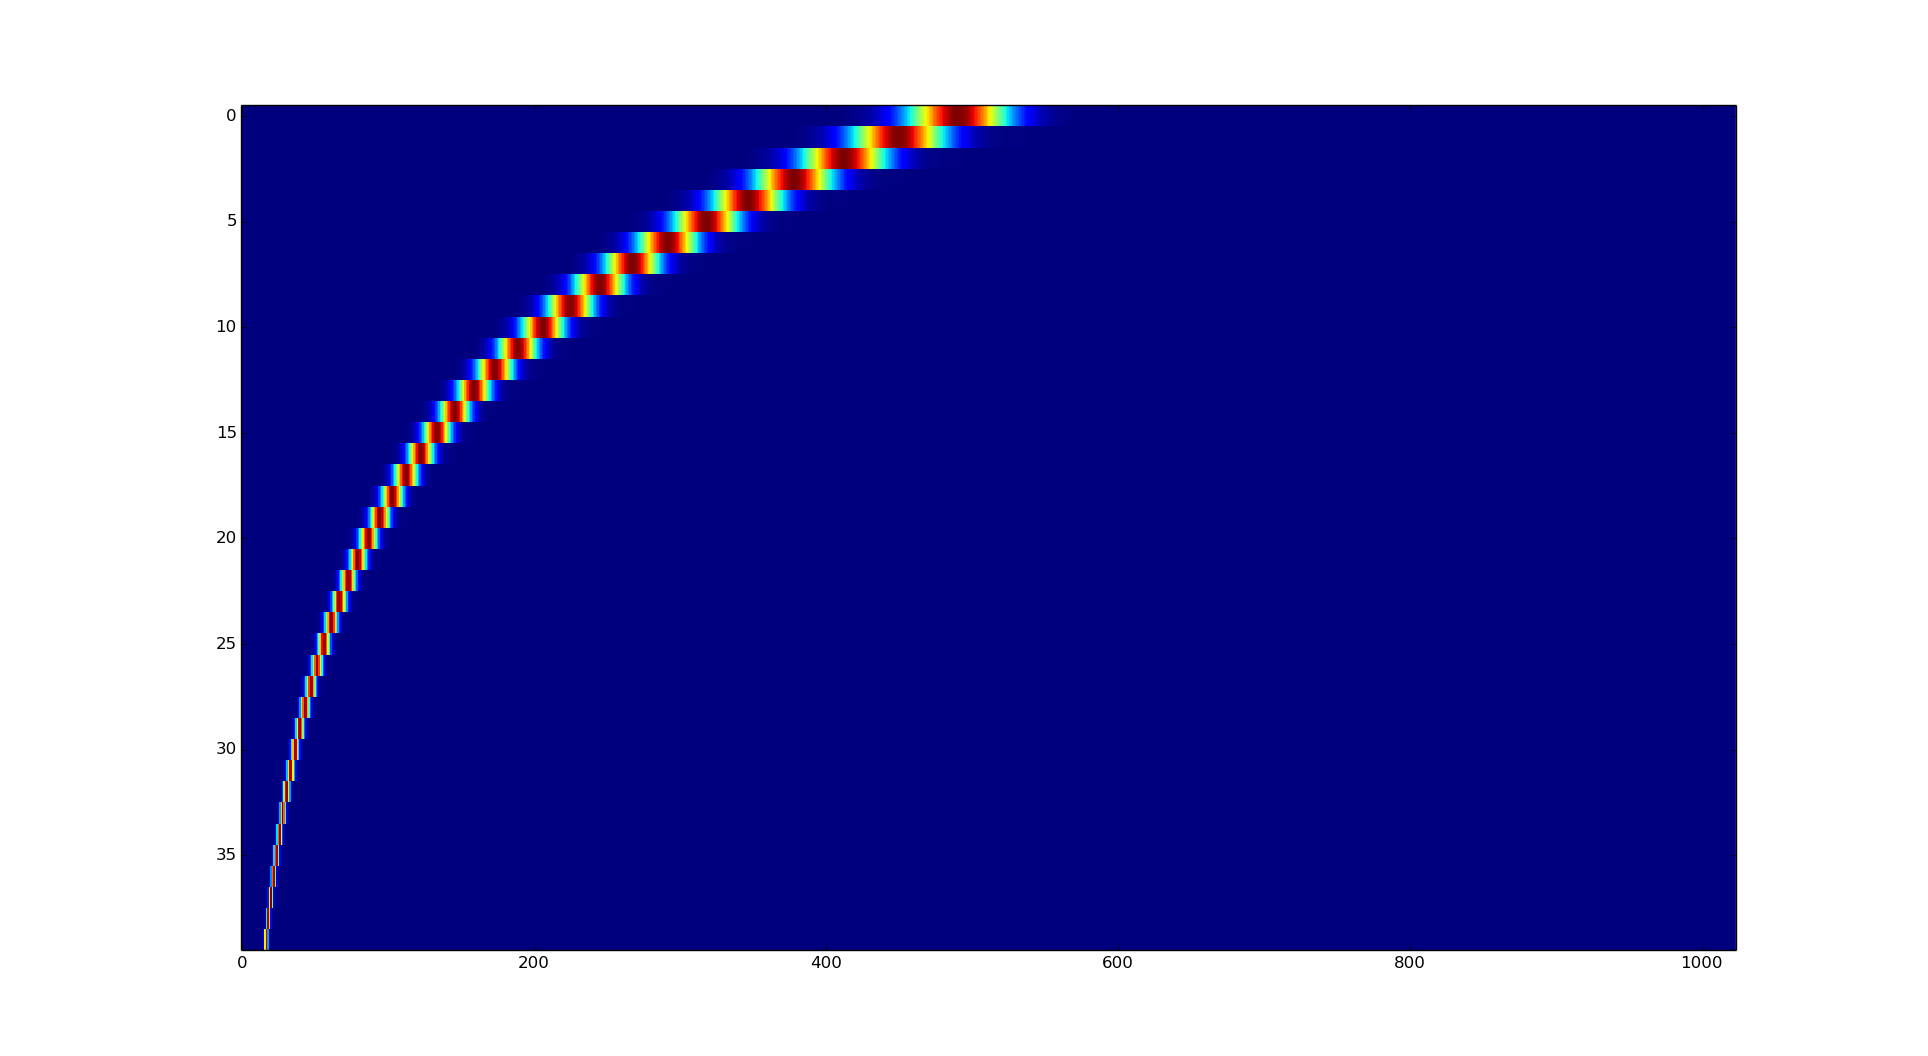
\includegraphics[scale=0.21]{psis.png}\caption{On 1024 bins, Q=8, J=5 without optimization on the support}\label{psis_examples}
\end{center}
\end{figure}

\section{Layer Implementation}\label{ll}
The role of this class is to be the link between the raw input, the meta parameters, and the filter banks by performing the decomposition process. Firstly, this class takes a $2D$ input (the input signal has to be transformed for the first layer). This allows an easy link between layers by directly setting the input of the next one as the output of the previous one. 
\\
Given the input, private variables are computed determining the structure of the class by computing variables that will be passed to the next layer such as the size of the output (given the input size and the number of $\psi$ filters :$Q*J$). Then when all the $\psi$ filters are available a Littlewood-Paley normalization is performed (due to the logarithmic spaced filters). After this, the filters are generated using the Filter1D class. The Decomposition can now be performed.
\\
Note that the decomposition is stored as a $2D$ matrix for every layer. Normally, layer $i$ has a dimension of $i+1$ which is not true in term of memory management. In fact, in this toolbox, the graph structure of the scattering network\ref{oo} has been kept through $2D$ matrices. For example for the second layer if we have $|\lambda_1|$ filters for the first layer and $|\lambda_2|$ filters for the second layer, the $U_2$ matrix of will be :
\[ U_2:= \left( \begin{array}{c}
||x \star \psi_{1,1}|\star \psi_{2,1}|\\
||x \star \psi_{1,2}|\star \psi_{2,1}|\\
\dots \\
||x \star \psi_{1,|\lambda_1|}|\star \psi_{2,1}|\\
||x \star \psi_{1,1}|\star \psi_{2,2}|\\
||x \star \psi_{1,2}|\star \psi_{2,2}|\\
\dots \\
||x \star \psi_{1,|\lambda_1|}|\star \psi_{2,2}|\\
\dots \\
||x \star \psi_{1,1}|\star \psi_{2,|\lambda_2|}|\\
||x \star \psi_{1,2}|\star \psi_{2,|\lambda_2|}|\\
\dots \\
||x \star \psi_{1,|\lambda_1|}|\star \psi_{2,|\lambda_2|}|\\
\end{array} \right)\]


\section{Scattering Network Implementation}
Finally here is how to perform the Scattering Network on a signal and to save the outputs :
\begin{lstlisting}
    MetaParam* opt=new MetaParam[3];
    opt[0]=MetaParam(8,30,4,1);
    opt[1]=MetaParam(64,1,1,1);
    opt[2]=MetaParam(1024,1,1,1);
    ScatteringNetwork decomposition("signal.wav",opt,3);

    ofstream file;
    file.open("layer1.txt");
    file<<decomposition[0];
    file.close();
    file.open("layer2.txt");
    file<<decomposition[1];
    file.close();
    file.open("layer3.txt");
    file<<decomposition[2];
    file.close();
    delete[] opt;
\end{lstlisting}
In fact the operator [] is overloaded to return the specific layer which itself uses its overloaded operator to export the coefficients.

\section{Optimizations and Computation Time}
\subsection{Filter Bank Optimizations}
Since we want to use this implementation on massive dataset, it is mandatory to optimize the implementation.

The best way to improve the required time to perform the decomposition is around the filters (allocation, creation, application,...). In fact, FFT/IFFT and the periodization algorithms already use efficient algorithms. 


I present here only the improvements concerning the filter bank, other details can be found in the C++ file comments.\\ 
The first big improvement is to only save in memory the coefficients of the filters that are not zero. So by only keeping the support of $\psi$ we can save memory but more importantly when we apply the operation $inputFFT .* \psi_{L,i}$ we only need to perform it on the support and set all the other coefficients to $0$. Doing this is really efficient by the natural sparsity of the filters as shown here : \ref{psis_examples}.
\\
Now that we only save part of the coefficients, the dimension is reduced and it is even possible to optimize again the filters creation. We know that filters are completely determined by the size of the input $N$ and the meta parameters $Q$ and $J$ for the $\psi$ filters. So in other word, it is possible to create a filter bank dictionary and save them in .txt files thus when we need some filters we only need to load them and not explicitly compute them over and over. This is particularly true since the input size must be a power of $2$ so there are not a huge number of input size that we can take as input.
By doing so, when we treat for example thousands of files, we will only load a few files without having to recompute the filters coefficients every single time.
Now, if we use the implementation in a loop over several signals, it is even possible to first load the filters and then perform all the decomposition without having to load filters every time too ! 
\\Note however that this optimization is not always usable. In fact, the use of this toolbox on other platform/servers or just because the user doesn't want IO operations for example, requires to actually compute the filters every time. In this case, the generating algorithm has been optimized using standard C++ optimization techniques such as loop-unrolling, inplace methods,...

\subsection{Computation Time}

Using all the available optimization without the use of the filter bank IO (thus generating the filters every time) this toolbox needs about $30\%$ of the signal duration (in second) to perform the loading of the wav, scattering decomposition and saving of the scattering coefficients into a .txt files). This required time obviously varies with the meta-parameters, the ones use here are the common ones (also used for the classification challenge presented later).
Note that using the filter bank IO will lead to better performance on huge dataset by not recomputing the filters for every signal.
The Scatnet implementation available in matlab requires $400\%$ of the signal time to perform the decomposition algorithm.
\\
Note that this toolbox is now used as the reference implementation for the scattering decomposition on ENS and UTLN servers for massive dataset decomposition (such as bioacoustic challenges). 
\section{Examples}
In the examples below we did not apply any operation (logarithm, re-normalization,...). The sub-plots are from top to bottom the
signal, and the $U_1$, $U_2$, $U_3$.
%\begin{figure}[H]
%\begin{center}
%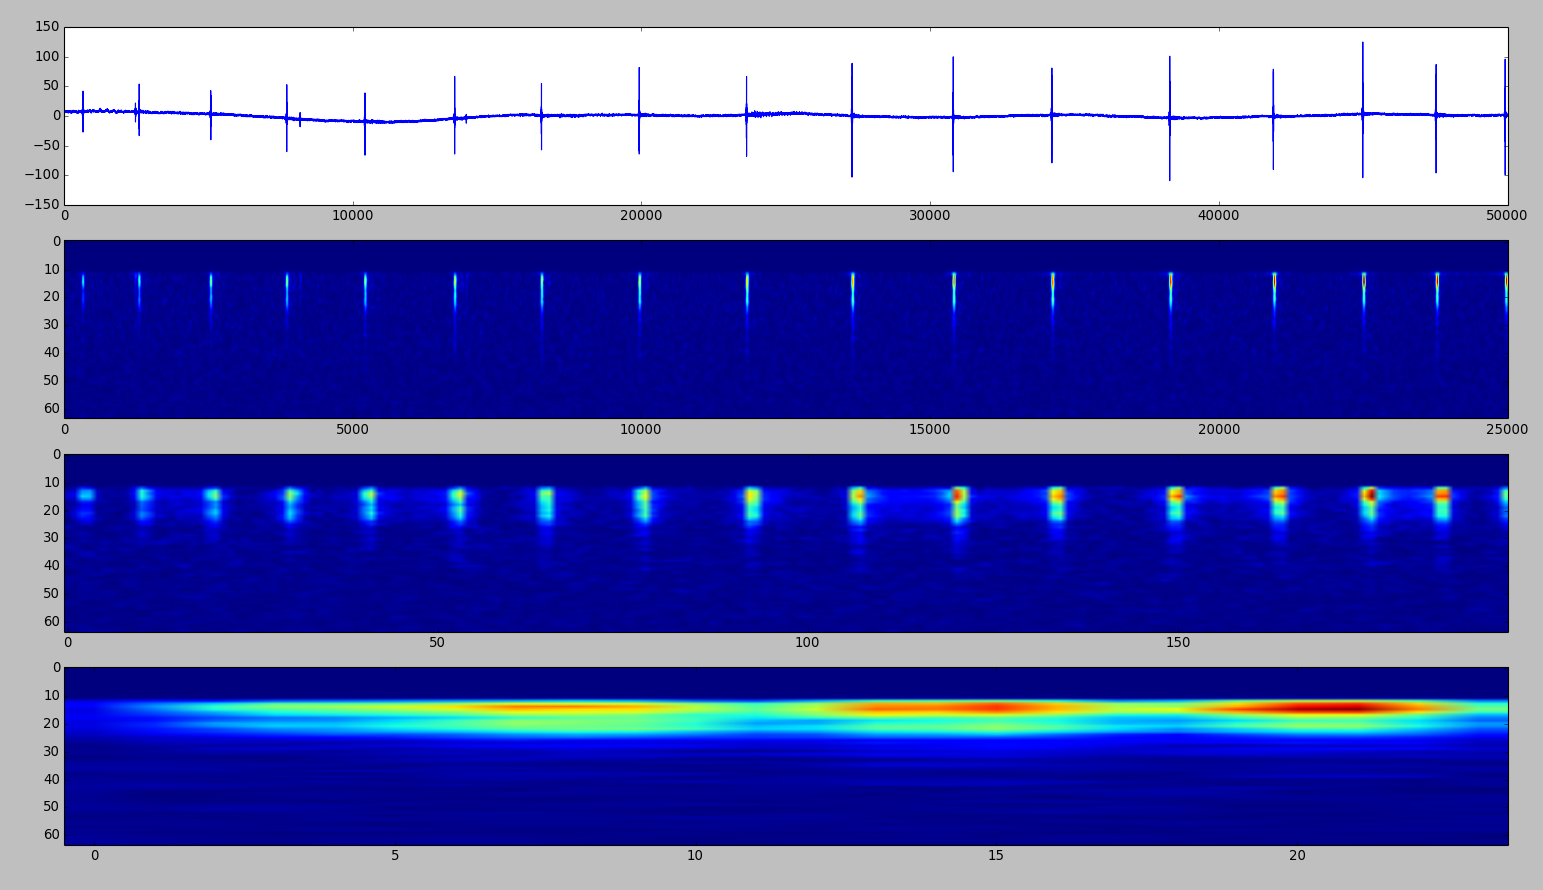
\includegraphics[scale=0.21]{slow.png}\caption{Signal (waveform), $U_1$, $U_2$, $U_3$ of Inia Perou \cite{trone2015}, a dolphin (slow clicks) T1:4 Q1:32 J1:2 T2:256 Q2:1 J2:1 T3:16 Q3:1 J3:1}
%\end{center}
%\end{figure}

%\begin{figure}[H]
%\begin{center}
%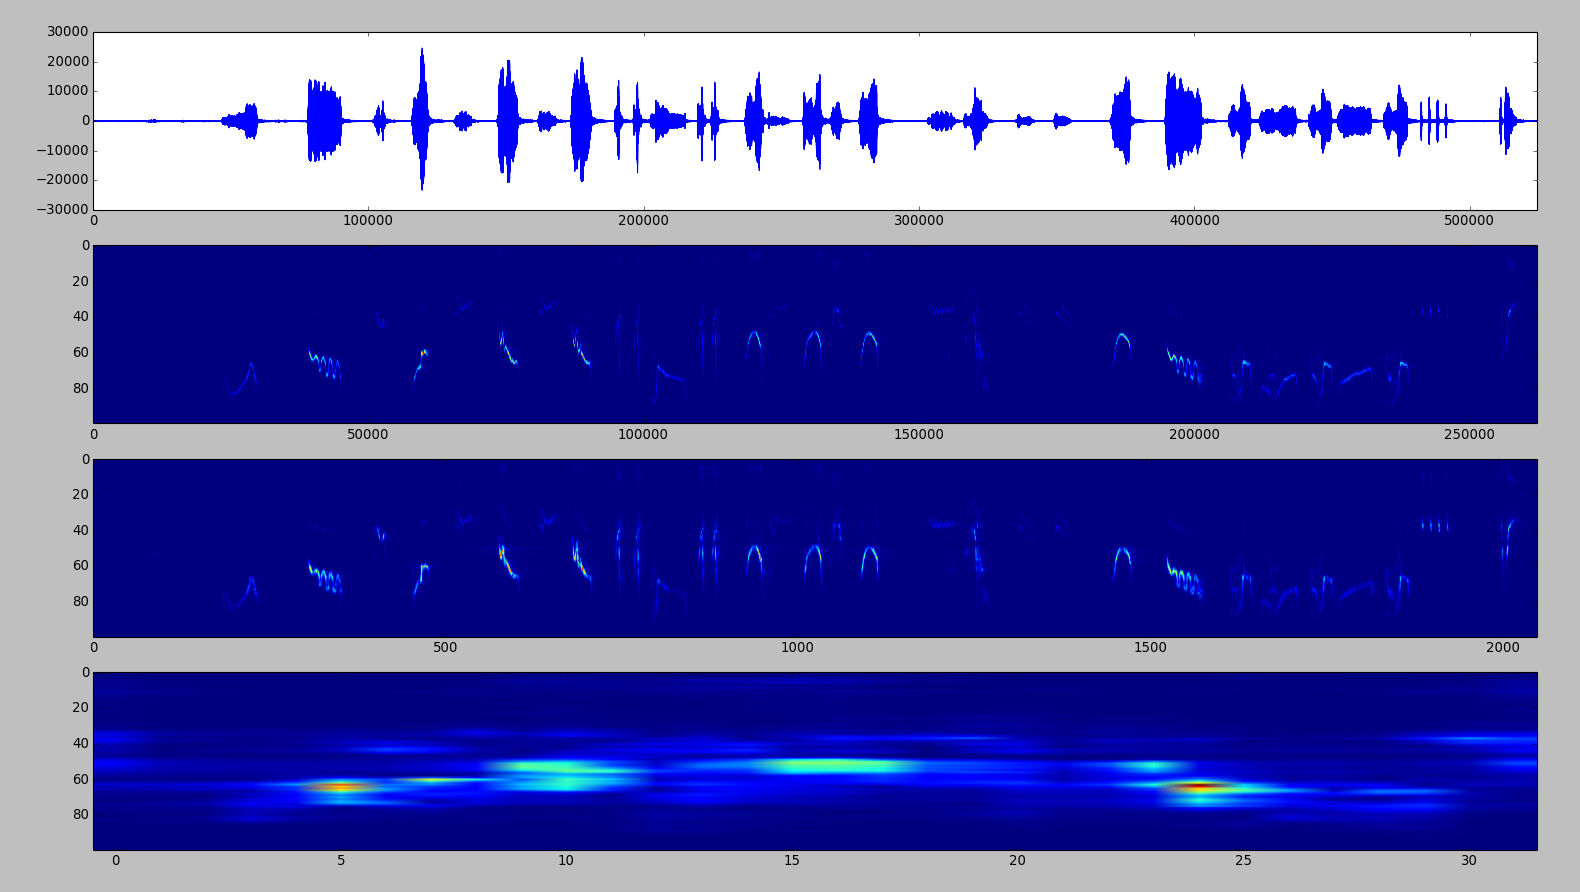
\includegraphics[scale=0.21]{bird.png}\caption{Signal (waveform), $U_1$, $U_2$, $U_3$ Bird (BIRDLIFE CLEF Challenge) T1:4 Q1:25 J1:4 T2:256 Q2:1 J2:1 T3:128 Q3:1 J3:1}
%\end{center}
%\end{figure}
\part{Benchmark and Bioacoustic Classification}


\part{Function parser}
\section{Motivation}
Throughout this library, we will need to parse functions in order to compute them explicitly. By functions we mean user-defined function given as a string and retrieved by a terminal interaction or through a Qt widget. In order to do this, multiple approaches can be used.\\
We want to be able to interpret any given function such as the string $f(x)=x^3-cos(x)$, in order to parse it, a binary tree is generated recursively on the given string with some simple rules (method used in this library). Another method (more related to compiler and language theory) implies the use of automaton.
\\
Note however that the parser is very basic and doesn't take into account operator priority so it is necessary to add parenthesis (as shown in the examples).
\section{Tree Generation}
\subsection{Rules}
The basic idea is to read a string from left to right and deduce what the current character stands for (this is done letter by letter).
This will be really simple since the only unknowns are $x$ and $y$ so any other letter which is not an operator can only be a function ($(e)xp,(s)in,...$).
To test if a character is an operator it is enough to test if the character is $+$, $-$, $*$, $/$ or power, thus the need of the two functions

\begin{itemize}
\item bool IsOp(char)
\item bool IsFunc(char)
\end{itemize}

Finally, note that if the character is a number, a utility function GetNumber will extract the number by taking all the following and adjacent characters that are numbers too. In fact, if the character is $5$ the next one can be another number if the user input was $58$ for example thus GetNumber("58+4*x") will return 58.\\
\subsection{Structure}
The generated tree will be made of nodes and leaves (the final nodes). A leaf can either be a constant (a number) or an unknown $x$ or $y$.\\
A node can be a function or an operator and will have two children (not necessarily leaves) for an operator node and only one for a function node. All of these structures inherit from a node class which provides an access operator() that will be accessed recursively to evaluate the parsed string (the generated tree).
\\



So let's look for example at the string $555+x$.
First we read $5$, it is a number so we look if the next character is also a number and so on to extract the whole plain number $\rightarrow$ extract $555$. \\
Now analyse the next character $+$ which generate an operator node where its two children are the string $555$ and $x$. The analysis is done recursively thus the string $555$ becomes a constant leaf and $x $ a variable leaf.
the access operator will then be used as $f(t)=555+t$ allowing the computation of the given string.\\
This was a really simple example but one can write for example
\[exp^{(cos(x)^2)/(sin(x)^2)}+N(0,1)
\]
It is important to note that the limits are taken into account, thus, plotting the tangent $sin(x)/cos(x)$ will given the right asymptotes.



The parenthesis are also important for operation priority since the operators are taken from right to left. This means that the multiplication is not, without parenthesis, computed first compared to an addition for example unless it is to the left of the addition. For example, $5*3+4$ will give $35$ and not $19$ so one has to write $(5*3)+4$.
it is interesting to know that this kind of priority and syntax (left-to-right) exists in arithmetic.
\section{Tree Evaluation}
When calling the access operator ()(float) there is a recursive call on all the children and the recursion stops on the leaves where an actual value is returned. Given our last example : $f(5) \rightarrow 555+(5)\rightarrow 560$. Obviously, only the variable leaf node will take into account the given value to the access operator, so the constant leaf $555$ will always return $555$ whereas the variable leaf $x$ will return the given value. 

\section{Implemented functions}
Some basic functions are already implemented. In addition, some random variables are also present and can be used really easily, for example, one can write $f(x)=x^2+N(0,1)$ meaning that for each given point, a standard normal distribution value will be generated and added to the value $x^2$. This can be useful to simulate some white noise for example or to add randomness...
\\
On the other hand, it is really easy to add some custom functions into the parser. For example one simply needs to add the function name (as a string) into the function list of the parser. This can allow use of custom functions. For example, if one wants to define $g$ a function returning $x^2$ it is possible to add it and then use in the parser the following string $f(x)=4*g(x+3)-2$ for example.\\
The already supported functions are :
\begin{itemize}
\item $exp$
\item $sin$
\item $cos$
\item $ln$
\end{itemize}

It is also possible to export the parsed function back into a string using some methods defined for the leaves/nodes. 
\section{Example}
Let's look at some examples :
\begin{lstlisting}[basicstyle=\tiny]
    PlainMatrix<> X;
    X=arange(-10,10,100);
    string h("45+x+225-20");
    string g("1+N(0,100)");
    Tree a(g);
    PlainMatrix<> Y;
    Y=a(X);
\end{lstlisting}

\part{Solver}

We will study the form
\[
Ax=b
\]
\[
A=\left( \begin{matrix}
a_{11}& a_{12} & ... & a_{1n}\\
a_{21}& a_{22} & ... & a_{2n}\\
&...&&\\
a_{n1}&a_{n2}&...&a_{nn}\\
\end{matrix} \right),
x=\left( \begin{matrix}
x_1\\
x_2\\
...\\
x_n
\end{matrix} \right),
b=\left(
\begin{matrix}
b_1\\
b_2\\
...\\
b_n
\end{matrix}
\right)
\]
Note that all the presented solvers are specialized for each shaped matrix when this implies a reduced computation time (by taking advantage of the special matrix shape).

\section{Direct Method}

\subsection{LU decomposition}
The most common method for solving the system $Ax=b$ is the Gauss pivot. When we save the pivot coefficient, it is called a $LU$ decomposition and is the most efficient direct method for exactly solving a matrix or finding its inverse (not taking count of round-off errors). It is provided for plain and sparse matrices. In order to solve a system with this method we need first to decompose a matrix into two triangular matrices and then use forward/backward substitution for solving.
\paragraph{Algorithms :}
Here are the substitution algorithms (forward and backward) : 
\\
\begin{algorithm}[H]
 \KwData{$L$,$b$}
 \KwResult{$x$}
 $x=b$\;
 $x[0]/=L(0,0)$\;
 \For{$i=1 \rightarrow N-1$}{
     \For{$j=0 \rightarrow i-1$}{
      $x[i]-=x[j]*L(i,j)$\;
      }
      $x[i]/=L(i,i)$\;
  }
 \caption{Forward Substitution with plain Matrix $O(N^2)$}
\end{algorithm}

\begin{algorithm}[H]
 \KwData{$U$,$b$}
 \KwResult{$x$}
 $x=b$\;
 $x[N-1]/=U(N-1,N-1)$\;
 \For{$i=N-2 \rightarrow 0$}{
     \For{$j=N-1 \rightarrow i+1$}{
      $x[i]-=x[j]*L(i,j)$\;
      }
      $x[i]/=L(i,i)$\;
  }
 \caption{Backward Substitution with plain Matrix $O(N^2)$}
\end{algorithm}
And now the decomposition algorithm storing the results into triangular matrices for efficient memory management. It would also be possible to store all the coefficient into one plain matrix with the upper triangular part and lower triangular being the two triangular matrices but since we have a triangular matrix class already implemented this will bring more flexibility.
\\
\begin{algorithm}[H]
 \KwData{$A$}
 \KwResult{$L$,$U$}
 $U=A$\;
 $L=diag(N)$\;
 \For{$k=0 \rightarrow N-1$}{
     \For{$i=k \rightarrow N-1$}{
     $L(i,k)=A(i,k)/A(k,k)$\;
     \For{$j=k\rightarrow N-1$}{
      $A(i,j)=A(i,j)-L(i,k)*A(k,j)$\;
      }
      }
  }
\caption{LU $O(N^3)$}
\end{algorithm}
Finally, for solving a system, the algorithm is as follow : first decompose the matrix and then solve $2$ systems with the triangular decompositions :
\begin{algorithm}[H]
 \KwData{$A$,$b$}
 \KwResult{$x$}
 $L,U=LU(A)$\;
 solve $ Ly = b$\;
 solve $ Ux = y$\;
\caption{Solve $O(N^3)$}
\end{algorithm}
Let's look at the following example, showing how to solve a linear system with this method.
\paragraph{Example}
\begin{lstlisting}[basicstyle=\tiny]



    PlainMatrix<> A(2,2);A(0,0)=1;A(0,1)=2;A(1,0)=-1;A(1,1)=2;
    cout<<A<<endl;
   
    /*
    1    2
    -1    2
   
    */

    Vector<> b(2);b[0]=1;
   
    LU_Decomposition<> LU(A);
    cout<<LU._L<<endl;
    /*
    1    0
    -1    1
    */
    cout<<LU._U<<endl;
    /*
    1    2
    0    4
    */
    cout<<LU.Solve(b)<<endl;
    //0.5    0.25



\end{lstlisting}
\subsection{Matrix Invert Computation}
Using the $LU$-decomposition can be used to invert a matrix.
In order to explicitly compute the inverse, the LU decomposition is done then followed by $2N$ forward-backward substitutions in order to solve $N$ systems (for each basis vector $e_i$). In fact we fill the $i^{th}$ column of the matrix inverse by computing the exact solution of
\[
Ax=e_i
\]
This leads to a possible computation of the inverse in $O(N^3)$
\subsection{Computing the Matrix Determinant}
In order to compute the determinant of large matrices, we compute the $LU$-decomposition and simply use the fact that :
\[
A=LU
\]
\[
det(A)=det(L)det(U)
\]
\[
\left( \prod_{i=1}^N L_{i,i} \right) \left(\prod_{i=1}^N U_{i,i}  \right)
\]
\section{Iterative Methods}
Direct solvers can become hard to use when dealing with large matrices, especially when sparsity is great and thus optimized algorithms are available. In order to reduce the computation cost (time and computational resources) one can use some iterative methods. Even though several methods exist, they all require some conditions (more strict than just $A$ being invertible) in order to converge almost surely.
\subsection{Jacobi}
One of the simplest method is the Jacobi method. The idea is to decompose $A$ into two matrices.
\[
A=D+R
\]

\[
D=\left(\begin{matrix}
a_{11} & 0 & ...& 0\\
0&a_{22}&...&0\\
 & & ... &\\
 0&0&...&a_{nn}
\end{matrix} \right)
,
R=\left(\begin{matrix}
0 & a_{12} & ...& a_{1n}\\
a_{21}&0&...&a_{2n}\\
 & & ... &\\
a_{n1}&a_{n2}&...&0
\end{matrix} \right)
\]

\[
Ax=b \implies (D+R)x=b \implies Dx=b-Rx \implies x^{k+1}=D^{-1}(b-Rx^k)
\]
\[
\rho(D^{-1}R)<1
\]
\begin{algorithm}[H]
 \KwData{$A$,$b$,$x_0$}
 \KwResult{$x_i$}
 $i=0$\;
 $D=D^{-1}$\;
 $a=Db$\;
 $b=-DR$\;
 \While{Criteria}{
 $ x^{i+1}=a+bx^k $\;
  }
 \caption{Jacobi}
\end{algorithm}

this algorithm converges if the matrix is strictly diagonally dominant.
Let's look at the approximated solution generated through this algorithm for solving a simple $2 \times 2 $ system :
\begin{figure}[H]
\begin{center}
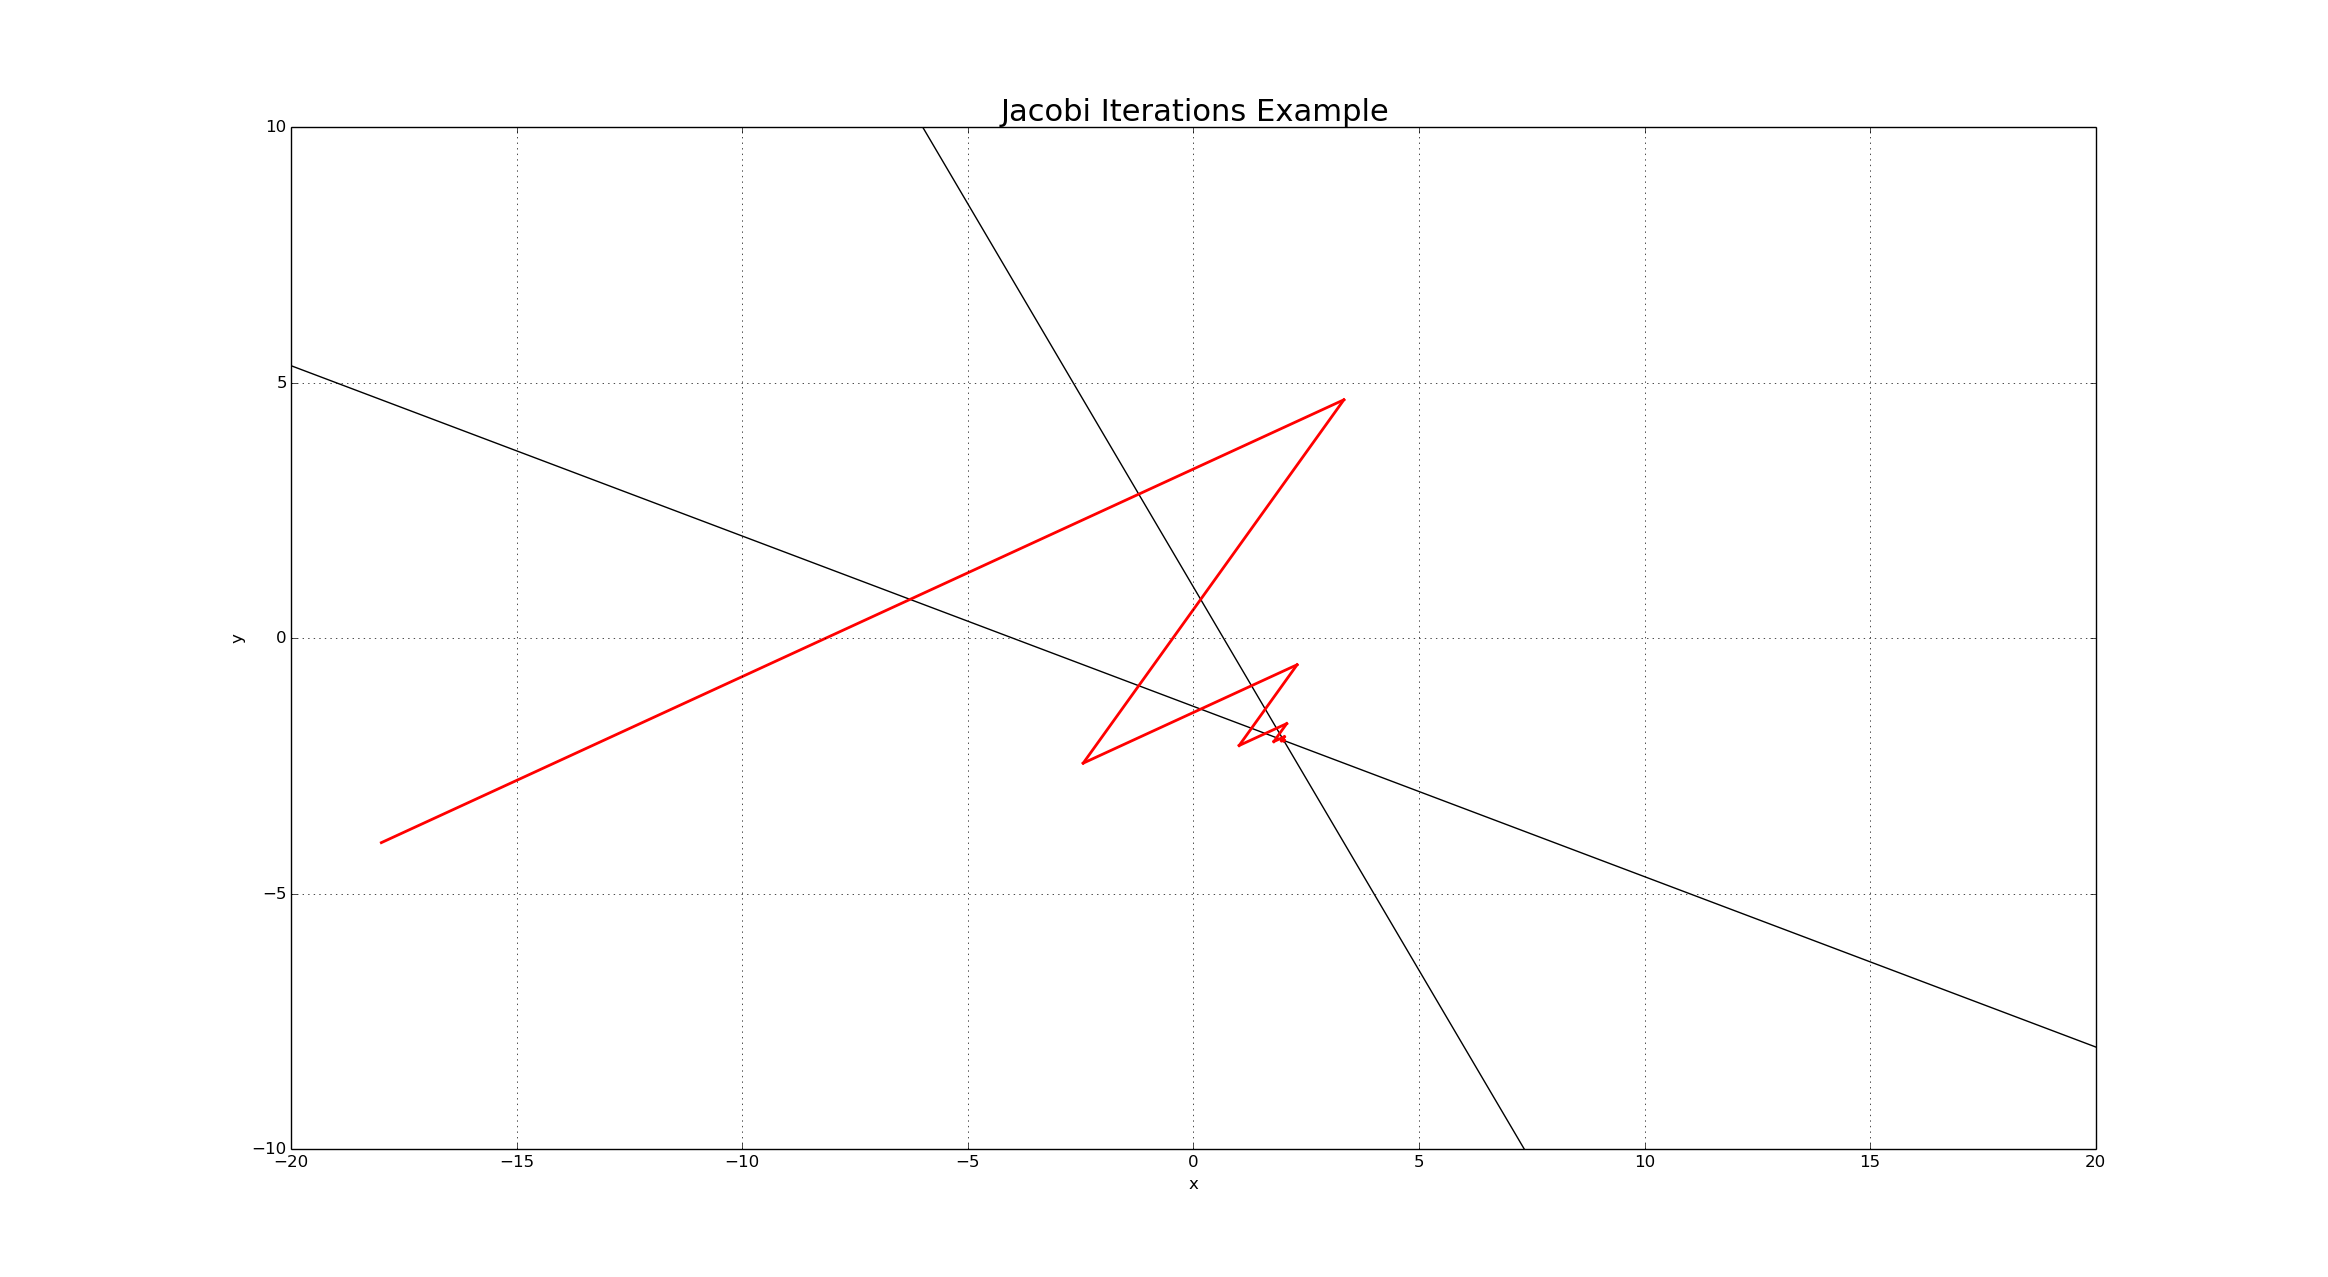
\includegraphics[scale=0.20]{jacobi_example.png}\caption{starting from $(-18,-4)$ to $(2,-2)$ in 24 iterations for an error of $1^{-10}$}
\end{center}
\end{figure}

And now the convergence of the method :
\begin{figure}[H]
\begin{center}
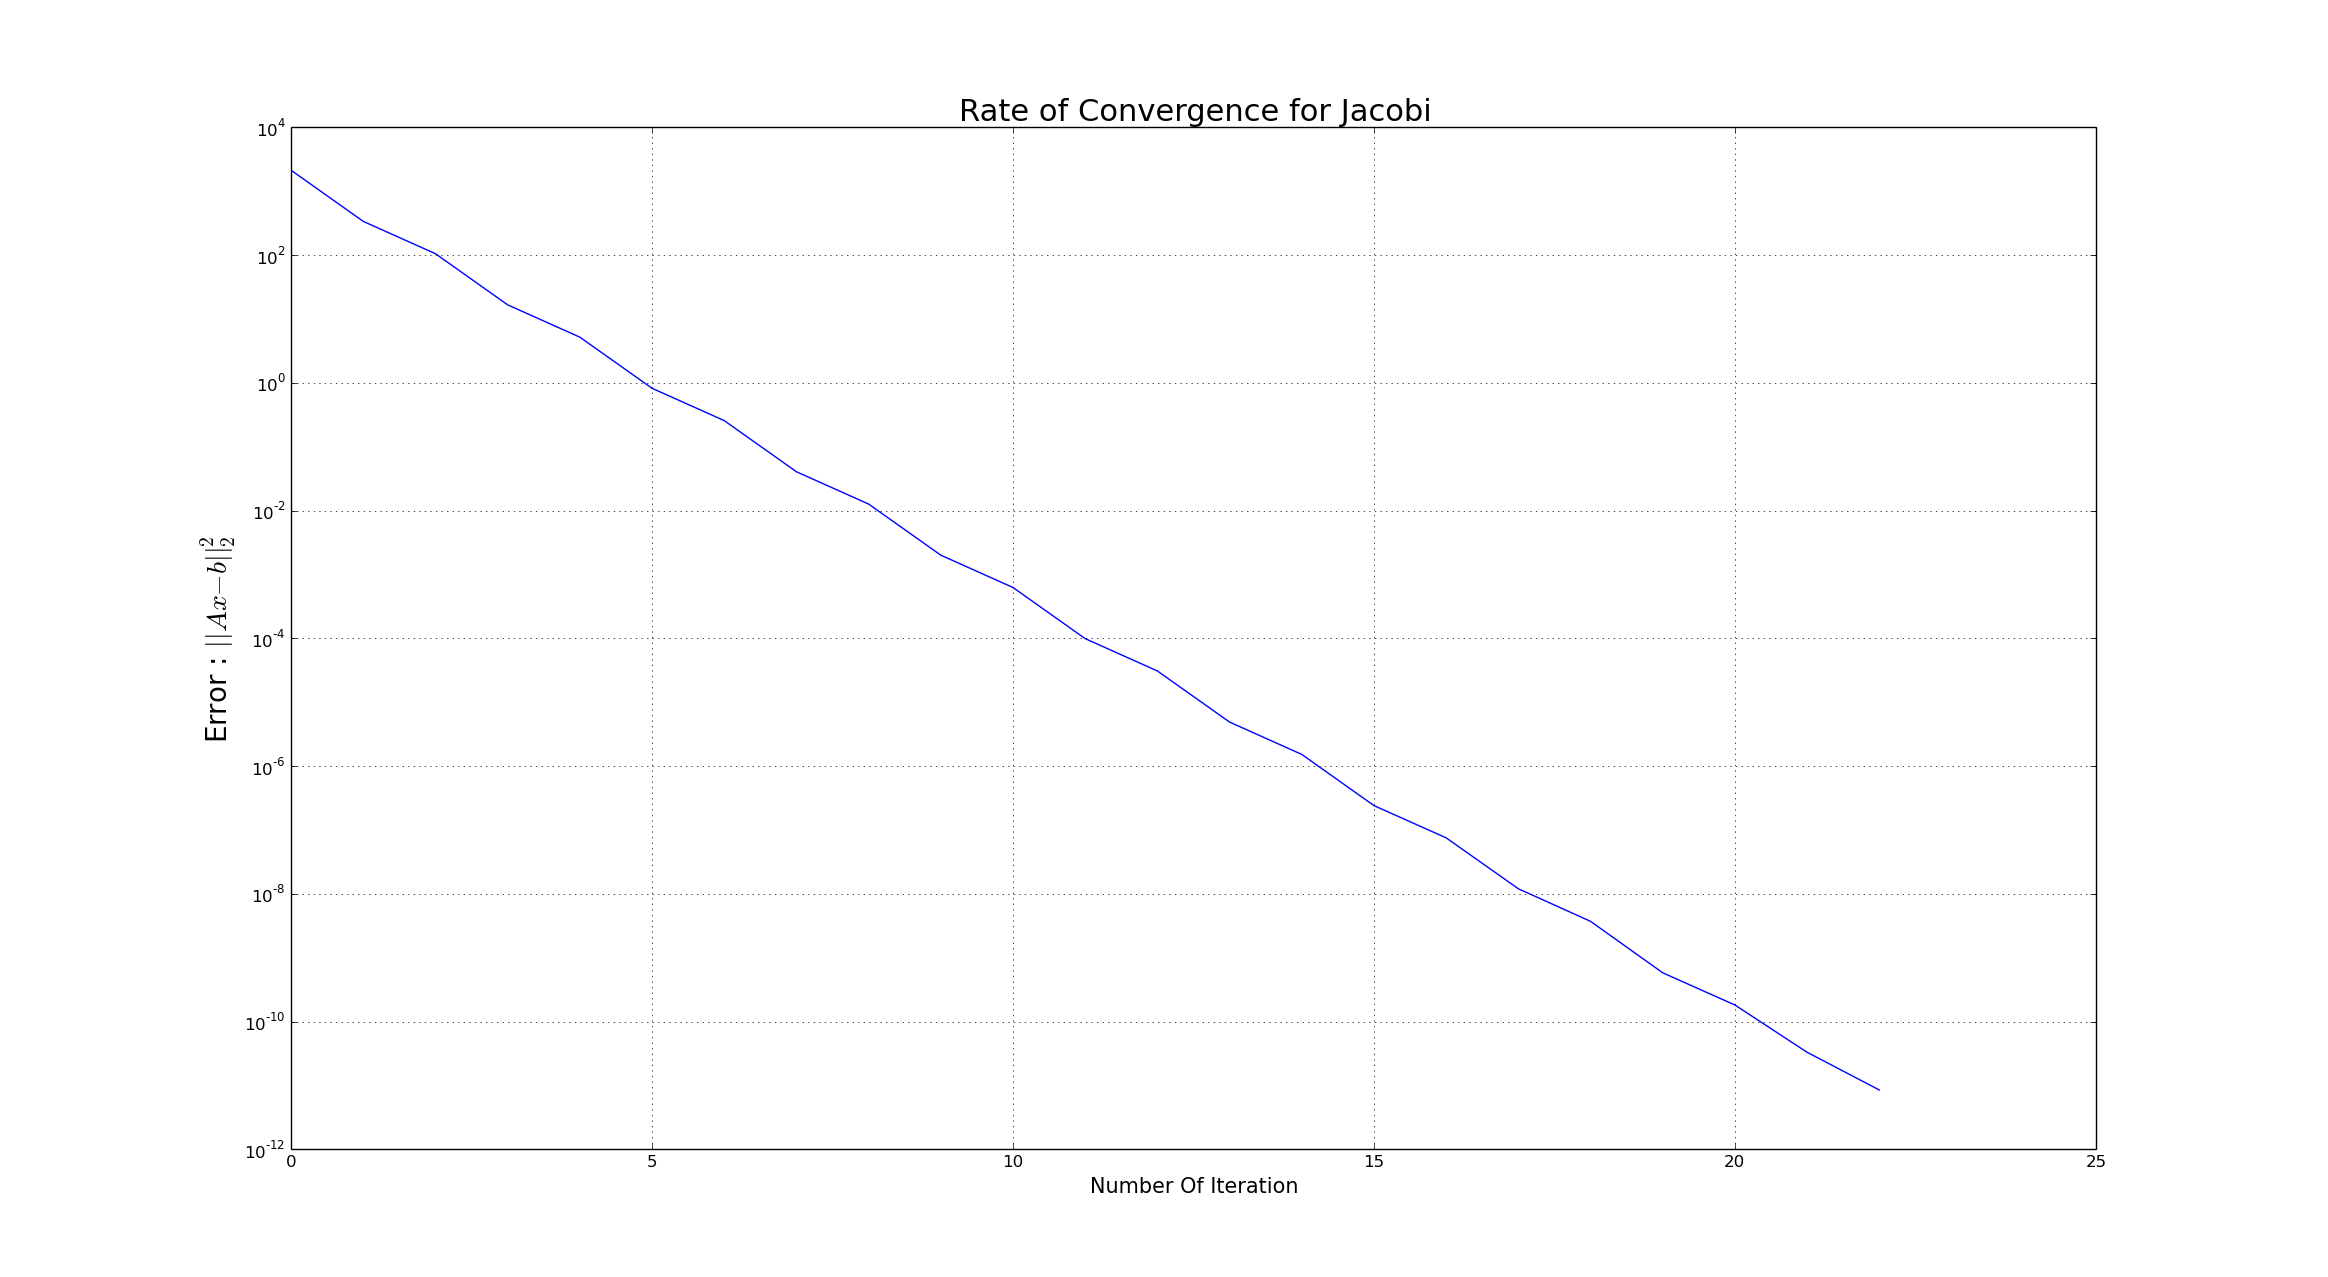
\includegraphics[scale=0.20]{jacobi_error.png}\caption{Error rate of the method which is plotted with a logarithmic y axis}
\end{center}
\end{figure}

\subsection{Gauss-Seidel}
We now decompose the matrix into two matrices and perform basically a similar algorithm to the Jacobi method but inside each iteration we use the already computed values for the computation of the other ones.
\[
A=L+U
\]
\[
L=\left(
\begin{matrix}
a_{11} & 0      & ... & 0 \\
a_{21} & a_{22} & ... & 0\\
& & ... &\\
a_{n1} & a_{n2} & ... & a_{nn}
\end{matrix}
\right) ,
U=\left(
\begin{matrix}
0 & a_{12} & ...    & a_{1n}\\
0 & 0      & ... & a_{2n}   \\
&&...&\\
0 & ...    &    ...     & 0
\end{matrix}
\right)
\]
\[
Ax=b \implies (L+U)x=b \implies Lx=b-Ux
\implies x^{k+1}=L^{-1}(b-Ux^k)
\]
\begin{algorithm}[H]
 \KwData{$A$,$b$,$x_0$}
 \KwResult{$x_i$}
 $i=0$\;
 $L=L^{-1}$\;
 $a=Lb$\;
 $b=-LU$\;
 \While{Criteria}{
 $ x^{i+1}=a+bx^k $\;
  }
 \caption{Gauss Seidel 1}
\end{algorithm}
This algorithm performs a plain $matrix * vector$ and a $vector+vector$ operation. The needed storage is for a plain matrix and a vector. Another algorithm could be
\\
\begin{algorithm}[H]
 \KwData{$A$,$b$,$x_0$}
 \KwResult{$x_i$}
 $i=0$\;
 $L=L^{-1}$\;
 \While{Criteria}{
 $ x^{i+1}=L(b-Ux^k) $\;
  }
 \caption{Gauss Seidel 2}
\end{algorithm}
In this case, we don't store a plain matrix but two triangular matrices and we perform two triangular $matrix* vector$ operations plus a $vector-vector$ operation which is about the same as the previous algorithm. However in this case there will be more cache miss.
To guarantee convergence, the matrix $A$ needs to be strictly diagonally dominant or symmetric positive definite. It is the same as SOR method with $\omega =1$.

Let's look at the approximated solution generated :
\begin{figure}[H]
\begin{center}
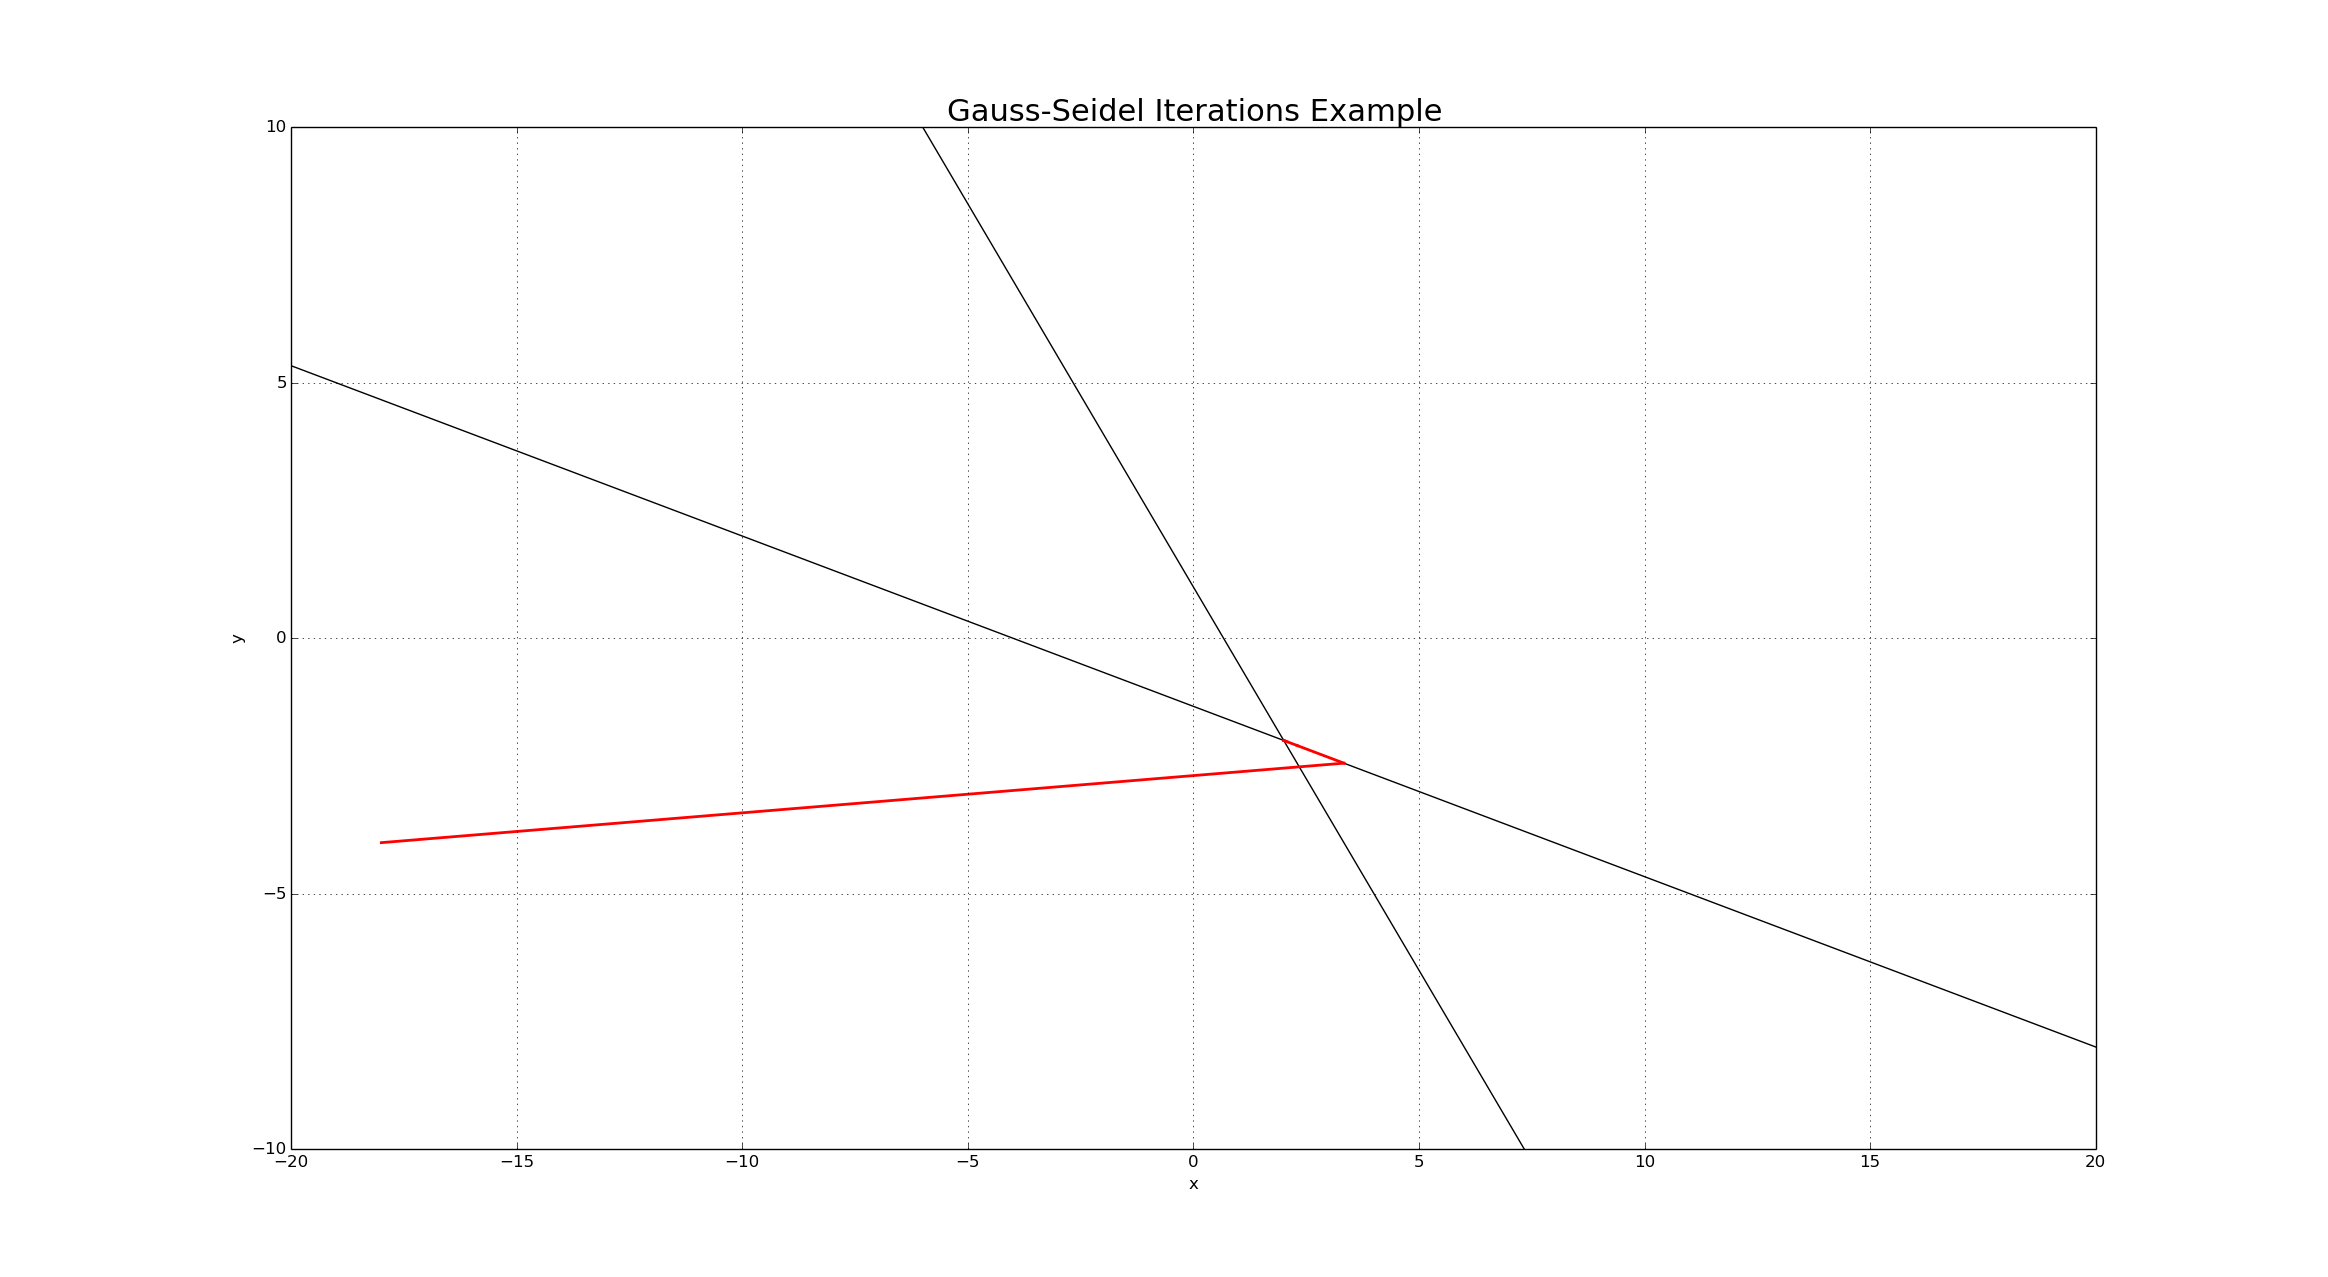
\includegraphics[scale=0.20]{gauss_seidel_iteration.png}\caption{starting from $(-18,-4)$ to $(2,-2)$ in 13 iterations for an error of $1^{-12}$}
\end{center}
\end{figure}
And now the convergence rate :

\begin{figure}[H]
\begin{center}
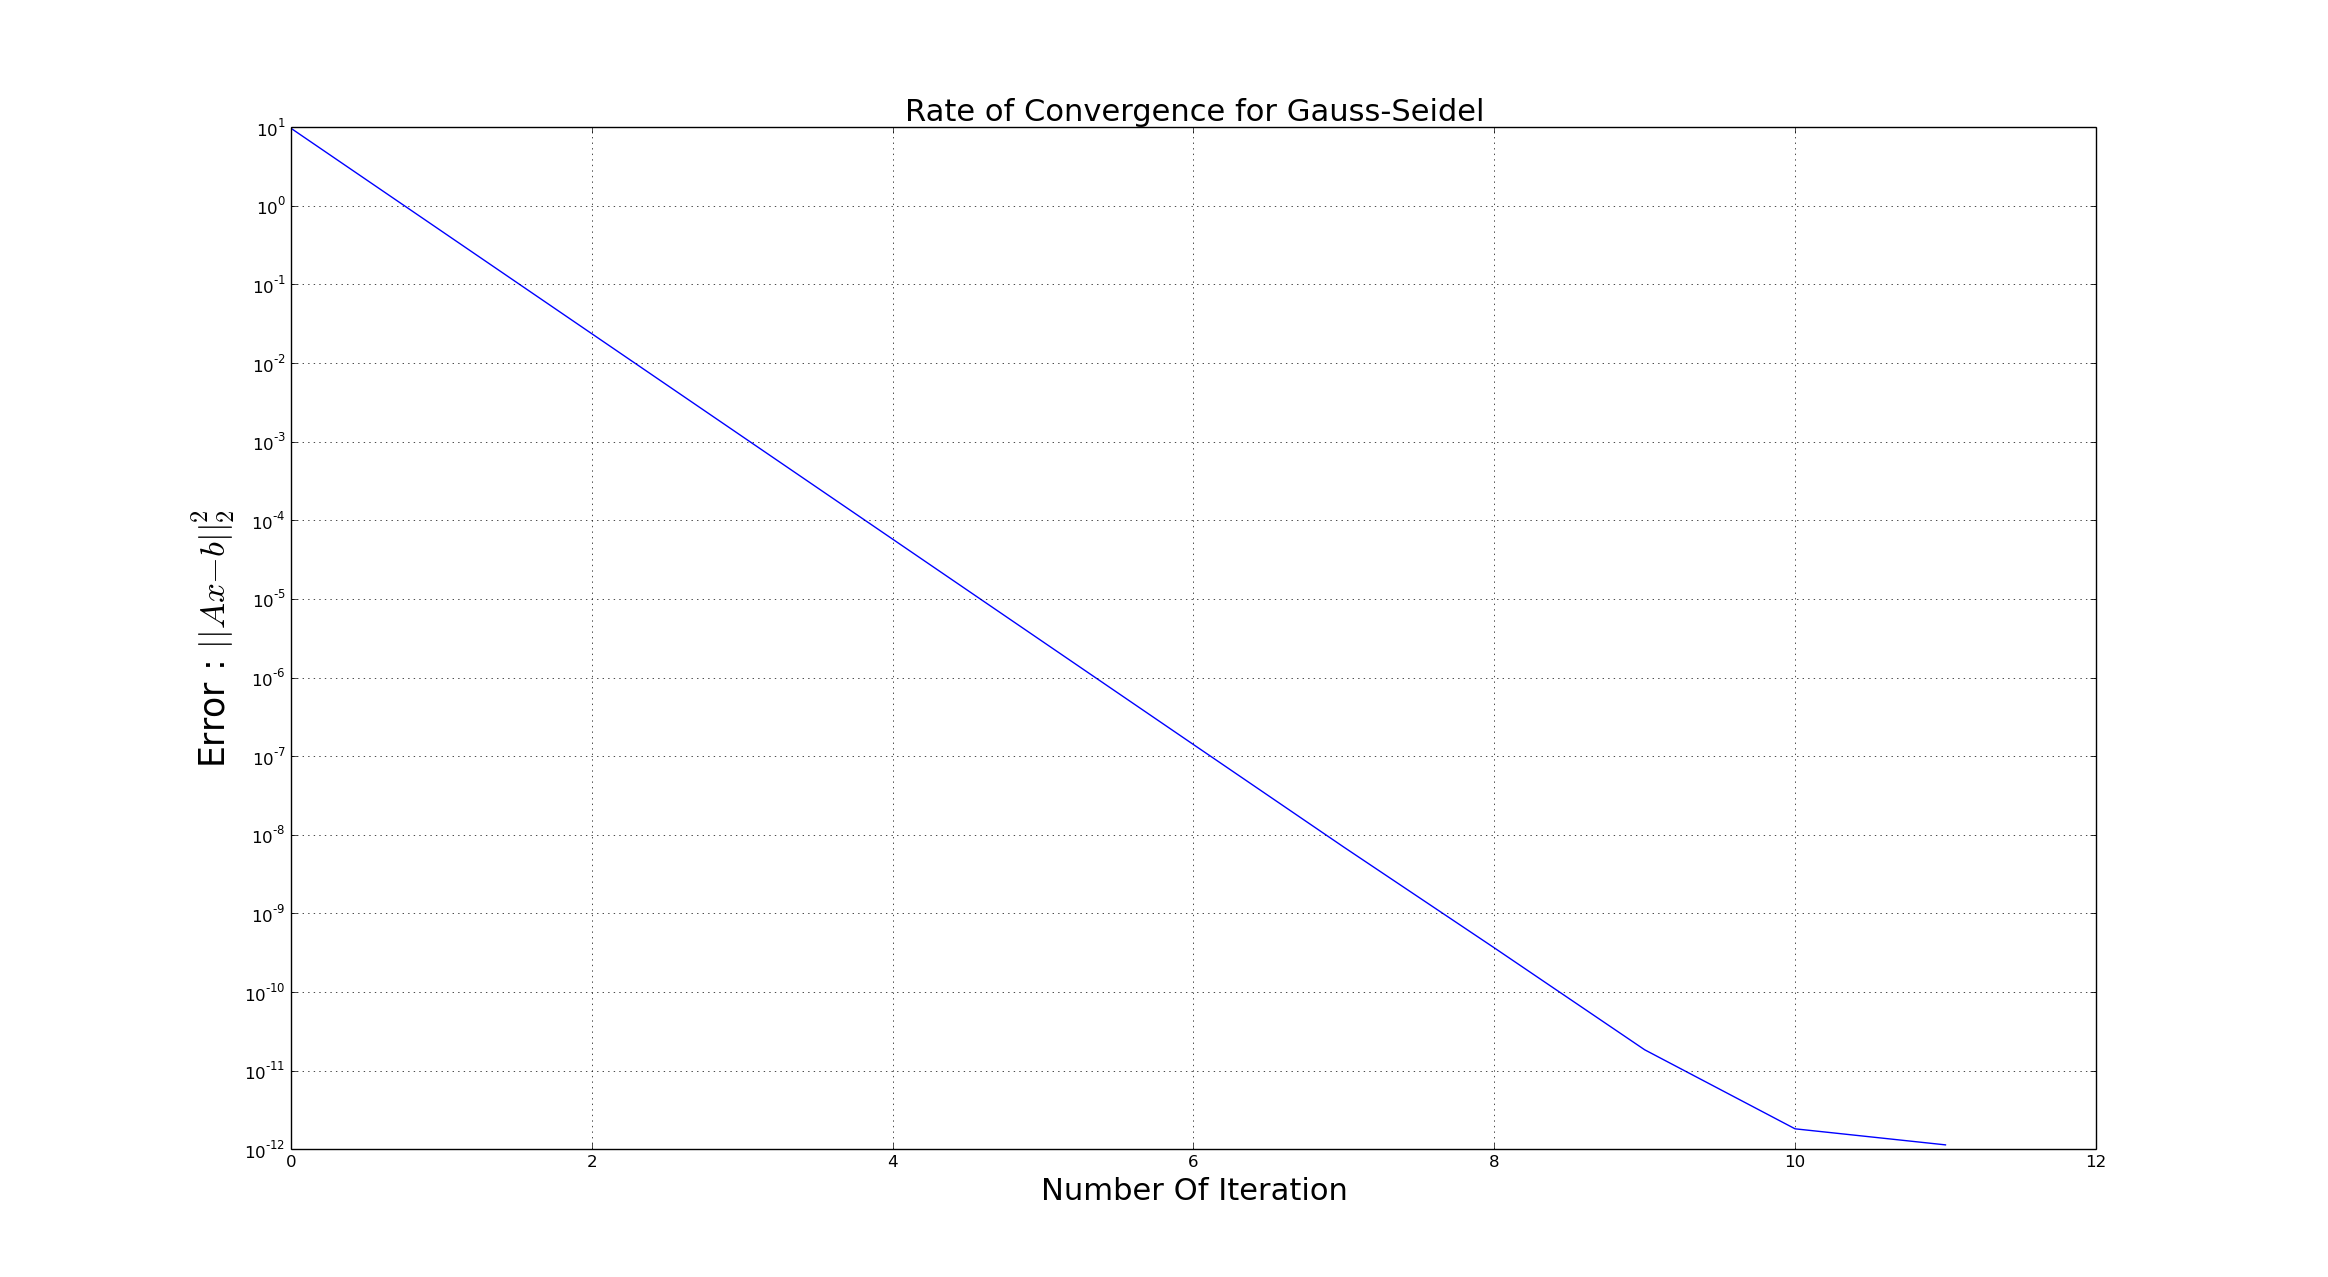
\includegraphics[scale=0.20]{gauss_seidel_rate.png}\caption{Error rate of the method which is plotted with a logarithmic y axis}
\end{center}
\end{figure}
here is the example used for this generation :
\begin{lstlisting}[basicstyle=\tiny]


    PlainMatrix<> A(2,2);
    BandMatrix<> Band(4,4,1);Band[0]=-1;Band[1]=2;Band[2]=-1;
//    cout<<Band<<endl;
    Vector<> B(2);B[0]=2;B[1]=-8;
    Vector<> X(2);X[0]=-18;X[1]=-4;
    A(0,0)=3;
    A(0,1)=2;
    A(1,0)=2;
    A(1,1)=6;
    cout<<GaussSeidel(A,B,X,0.000000000001)<<endl;


\end{lstlisting}
\subsection{Successive Over Relaxation}
Finally another simple method based on Gauss-Seidel is the SOR-method which is not implemented in this library :
\[
A=D+L+U
\]
\begin{align*}
&Ax=b \\
\implies & \omega Ax=\omega b \\
\implies & \omega \left( D+L+U \right) x=\omega b\\
\implies & \left( D \omega +L \omega + U \omega \right)x = \omega b\\
\implies & \left( D-(1- \omega)D +L\omega +U\omega \right)x =\omega b\\
\implies & \left( D+ \omega L \right) x^{k+1}=\omega b + \left( (1-\omega)D-\omega U \right)x^k\\
\implies & x^{k+1}=\left( D+ \omega L \right)^{-1} \left( \omega b + \left( (1-\omega)D-\omega U \right)x^k \right)
\end{align*}
This leads to the following algorithm :
\\
\begin{algorithm}[H]
 \KwData{$A$,$b$,$\omega$,$x_0$}
 \KwResult{$x_i$}
 $i=0$\;
 $L=(D+\omega L)^{-1}$\;
 $a=\omega Lb$\;
 $b=L\left[ (1-\omega)D-\omega U  \right]$\;
 \While{Criteria}{
 $ x^{i+1}=a+bx^k $\;
  }
 \caption{SOR Relaxation}
\end{algorithm}
The difficult part in this algorithm is to find the optimal $\omega$ leading to the fastest convergence rate.
\section{Gradient Based Methods}
In order to solve the linear system $AU=F$ that will be generated in the application, we need to use an iterative method which will be useful since $A$ will be sparse. \\in the following cases,
we aim to solve the system $Ax=b$ by minimizing the function
\[
f(x)=x^TAx-b^Tx+c
\]
Thus finding the point where the gradient is $0$ :
\[
\nabla f(x)=Ax-b=0
\]
\[
\Delta f(x)=A
\]
In order to do this we will use two methods : Gradient Descent and Conjugate Gradient Descent. In order to apply these methods, $A$ must be symmetric positive definite. So there exists a unique minimum since the Hessian of the considered function is $A$.
Let's first illustrate these approaches using some $2D$ examples.
\begin{figure}[H]
\begin{center}
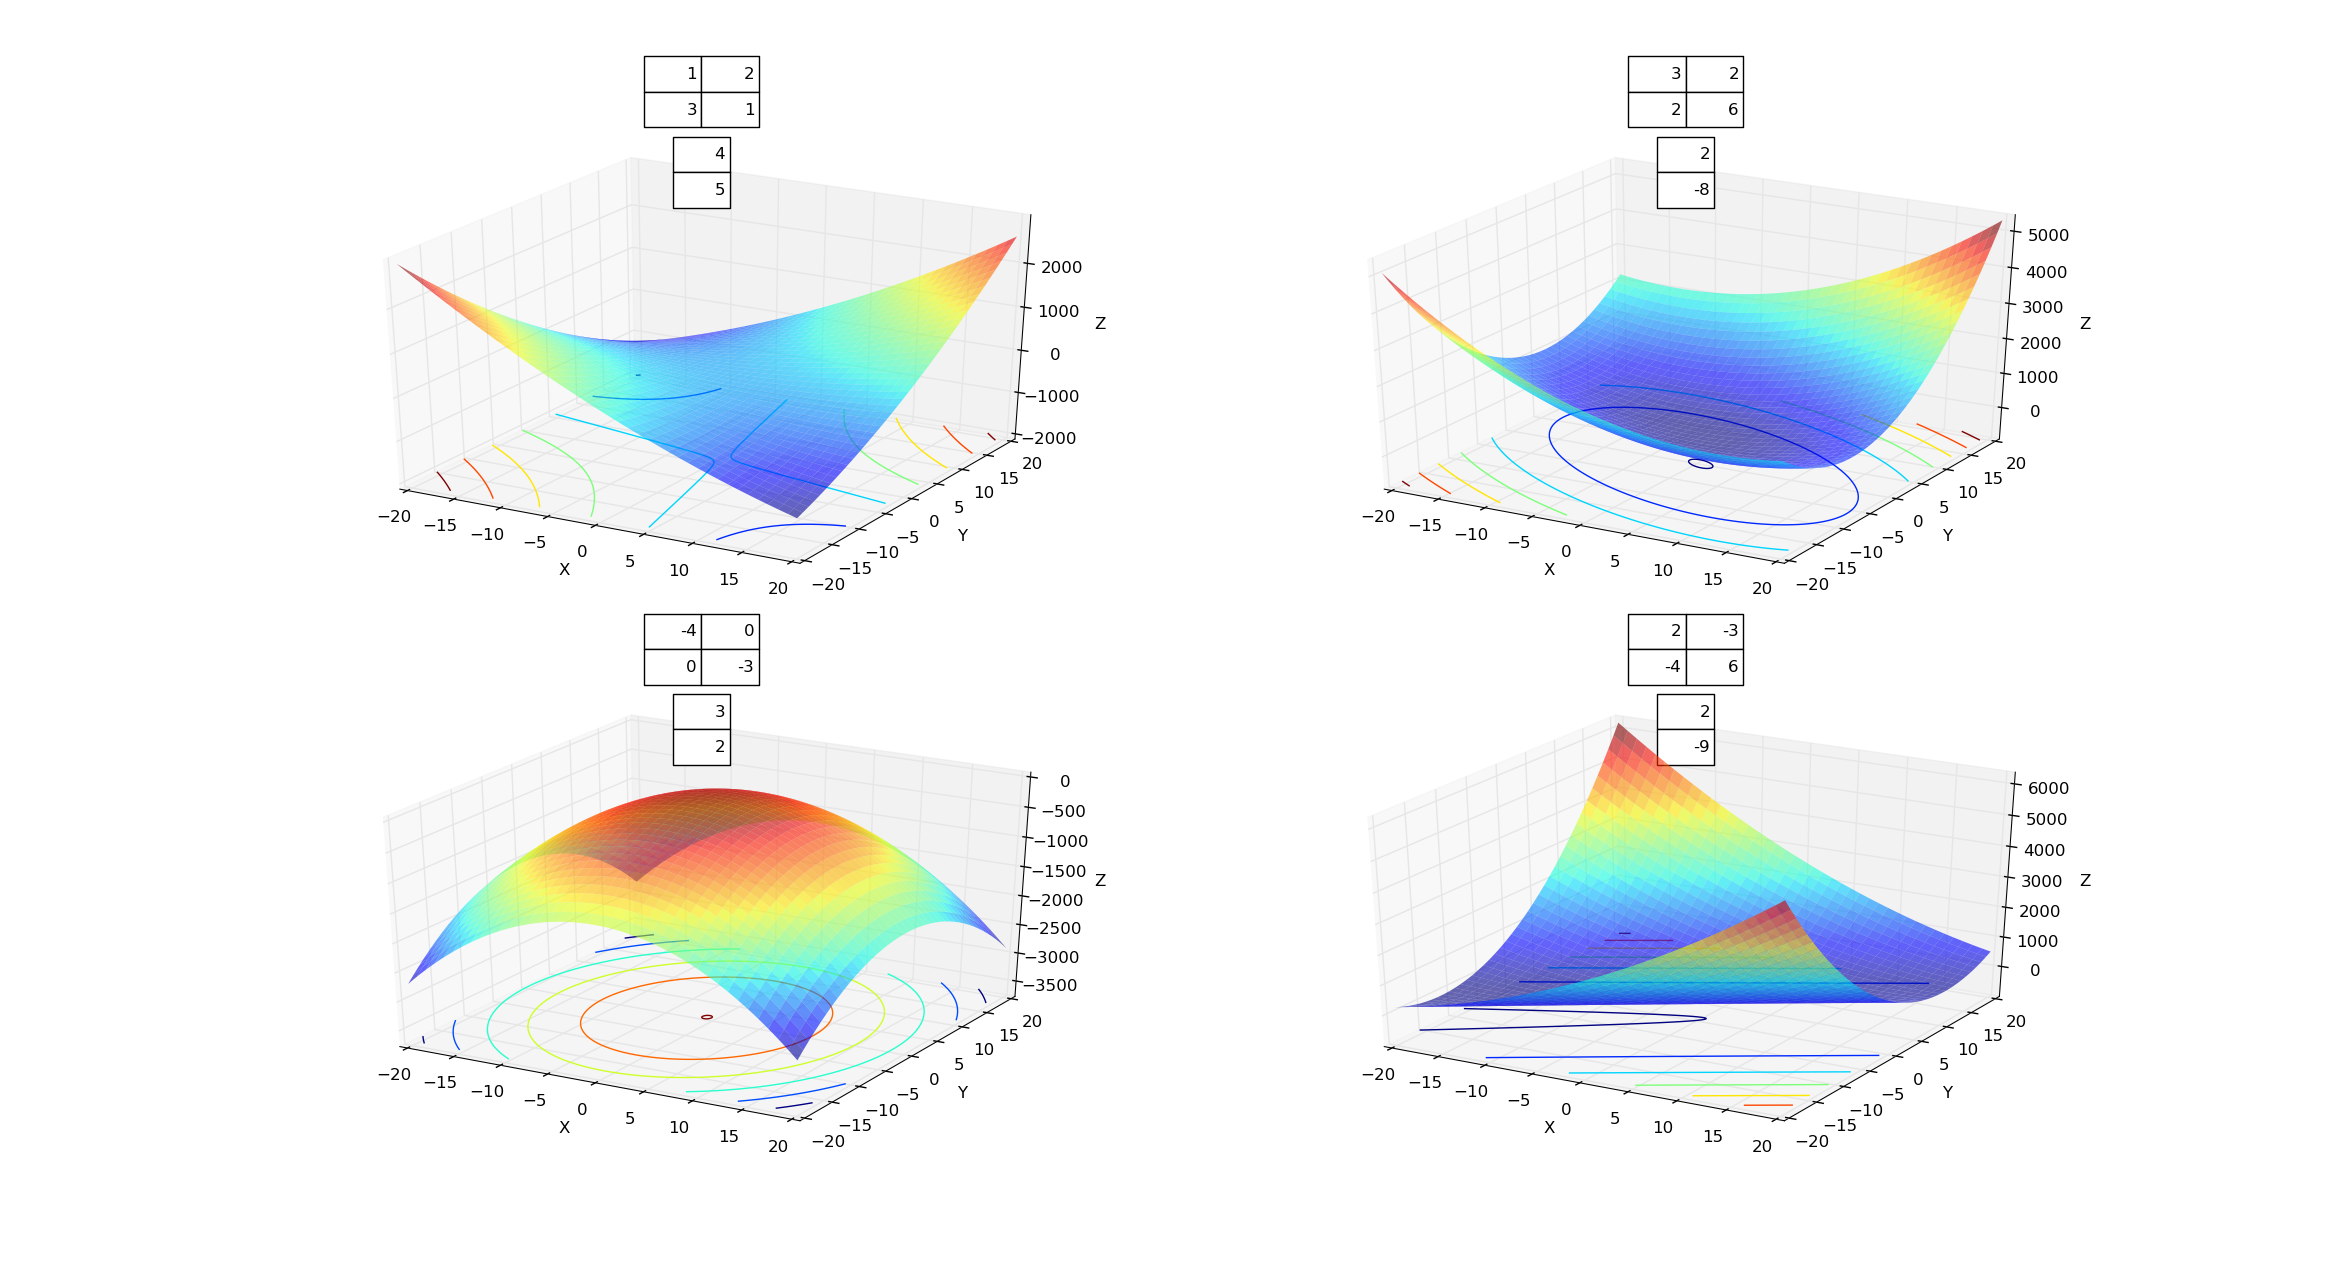
\includegraphics[scale=0.20]{courbes.png}\caption{Examples of the function to minimize with different matrices}
\end{center}
\end{figure}
The first matrix shows a saddle point, the second one is symmetric positive definite thus has one global minimum, the third one is symmetric negative definite thus having one global maximum. Finally, the last one has no solution thus no extrema. This is why this condition is important.
\\
Note that for all the methods, the mandatory argument is only the function to generate $F$ but optional arguments are : diagonal preconditioning, $\epsilon$ : the stop criteria and $C$ the number of iterations between criteria check. By default $\epsilon=10^{-12}$ and $C=10000$ for the GD and $100$ for the CGD.
\subsection{Gradient Descent}
The main idea of the gradient descent is to find the nearest local (or in this case global) minimum by using the gradient. At each iteration we follow the gradient opposite direction and perform a line search. This line search provides the minimum of $f$ in this direction. The scheme is as follow, go from $x_k$ to $x_{k+1}$ with the relation $x_{k+1}=x_k-\alpha_k\nabla f(x_k)$ with $\alpha_k$ being the result of the line search :
\begin{align*}
&\frac{\partial f}{\partial \alpha_k}(x_k-\alpha_k \nabla f(x_k) =0\\
\implies &- \nabla f(x_k) \nabla f(x_k-\alpha_k \nabla f(x_k))) =0 \\
\implies&- \nabla f(x_k)\left( A(x_k-\alpha_k \nabla f(x_k))-b)  \right) =0 \\
\implies&- \nabla f(x_k)^T \nabla f(x_k)+\alpha_k \nabla f(x_k)^TA \nabla f(x_k)=0\\
\implies&\alpha_k = \frac{\nabla f(x_k)^T \nabla f(x_k)}{ \nabla f(x_k)^TA \nabla f(x_k)}
\end{align*}
Note that the consecutive descent directions are orthogonal.
\\
\begin{algorithm}[H]
 \KwData{$A$,$b$,$x_0$}
 \KwResult{$x_i$}
 $i=0$\;
 \While{Criteria}{
 $\alpha_i=\frac{\nabla f(x_i)^T \nabla f(x_i)}{\nabla f(x_i)^T A \nabla f(x_i)}$\;
 $x_{i+1}=x_i-\alpha_i \nabla f(x_i)$\;
 $i=i+1$\;
  }
 \caption{Deepest Descent Algorithm}
\end{algorithm}
With $\nabla f(x_k)=Ax_k-b$ and obviously
 $\nabla f(x_{k+1})=A x_{k+1}-b =   \nabla f(x_k)- \alpha_i  A \nabla   f(x_i)$ to save one matrix vector product. So an optimized algorithm could be
 \\

\begin{algorithm}[H]
 \KwData{$A$,$b$,$x_0$}
 \KwResult{$x_k$}
  $g=\nabla f(x_0)=Ax_0-b$\;
 \While{Criteria}{
 $ p = Ag$\;
 $\alpha=\frac{g^T g}{g^T p}$\;
 $x-=\alpha_i g$\;
 $g-=\alpha_i p$\;
  }
 \caption{Deepest Descent Algorithm}
\end{algorithm}
With the last two inplace subtractions being made simultaneously in order to not compute two times the same value. Note that in this case we avoid to explicitly compute $\nabla f(x^{k+1})$ by using the recursive formula, however this can lead to more round-off errors.
Also, stop criteria can be checked every $C$ iterations and not every time. When it is being check, we also update the gradient with the standard formula to reset the accumulated round-off errors.
\\
Illustration of the method applied to the second matrix of the previous image :




\begin{figure}[H]
\begin{center}
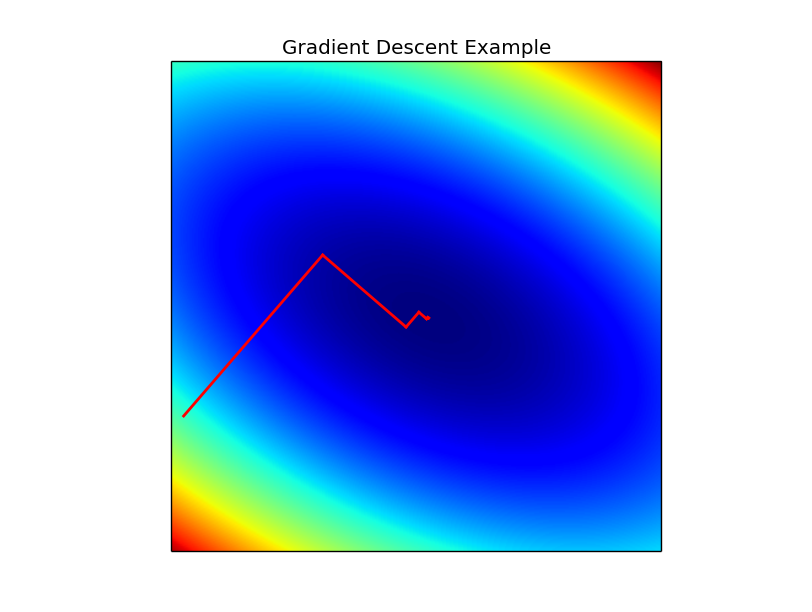
\includegraphics[scale=0.40]{GD_example.png}\caption{Gradient Descent iterations}
\end{center}
\end{figure}

Here is how to use the method (one can actually use the function GD as a stand alone by providing the input variables).
This method will take a function pointer as the first input in order to create the $F$ vector (here the function is a simple $sin(3x)$). The second (and optional) input is the diagonal preconditioning, described in \ref{precon}.
\begin{lstlisting}[basicstyle=\tiny]
    double F(double const& x){
           return sin(3*x);
    }
    Mesh1D<double> mesh(0,2*M_PI,20000);
    MatriceTridiagonale<double> A(20000,Triple<double> (-1,2,-1));
    A._Mesh=&mesh;
    A.GDSolve(F);
\end{lstlisting}
\subsection{Conjugate Gradient Descent}
The idea now is not to follow orthogonal descent directions but $A-$orthogonal directions. A vector $x$ is $A-$orthogonal (or conjugate) if $x^T A x=0$. We will denote these new directions by $p$. The first $p$ is the gradient, but then $p_{i+1}$ is computed so it is a conjugate of $p_i$.
\\

\begin{algorithm}[H]
 \KwData{$A$, $b$, $x_0$}
 \KwResult{$x_i$}
 $p_0=- \nabla f(x_0)$\;
 \While{Criteria}{
 $\alpha_i = \frac{\nabla f(x_i)^T p_i}{p_i^TAp_i} $\;
 $x_{i+1}=x_i- \alpha_i p_i$\;
 $\lambda = \frac{\nabla f(x_{i+1})^T\nabla f(x_{i+1})}{\nabla f(x_{i})^T\nabla f(x_{i})}$\;
 $p_{i+1}=\lambda p_i- \nabla f(x_{i+1})$\;
  }
 \caption{CGD algorithm}
\end{algorithm}
With $\nabla f(x^{k+1})=Ax^{k+1}-b=\nabla f(x^k-\alpha ^kp^k)=\nabla f(x^k)-\alpha^kAp^k$
\\
\begin{algorithm}[H]
 \KwData{$A$, $b$, $x_0$}
 \KwResult{$x_i$}
 $x=x_0$\;
 $g_0=\nabla f(x)=Ax-b$\;
 $p=- g$\;
 \While{Criteria}{
 $t=Ap$\;
 $\alpha_i = \frac{g_0^T p}{p^Tt} $\;
 $x-=\alpha p$\;
 $g_1=g_0- \alpha t$\;
 $\lambda = \frac{g_1^T g_1}{g_0^T g_0}$\;
 $p=\lambda p-g_1$\;
 $g_0=g_1 $\;
  }
 \caption{Optimized CGD algorithm}
\end{algorithm}
Once again by using the recursive formula for the gradient, errors might accumulate, thus it is refreshed when checking for the stop criteria. Note that the CGD converges much faster than GD.
\\
Illustration of the method on the same 2D matrix :


\begin{figure}[H]
\begin{center}
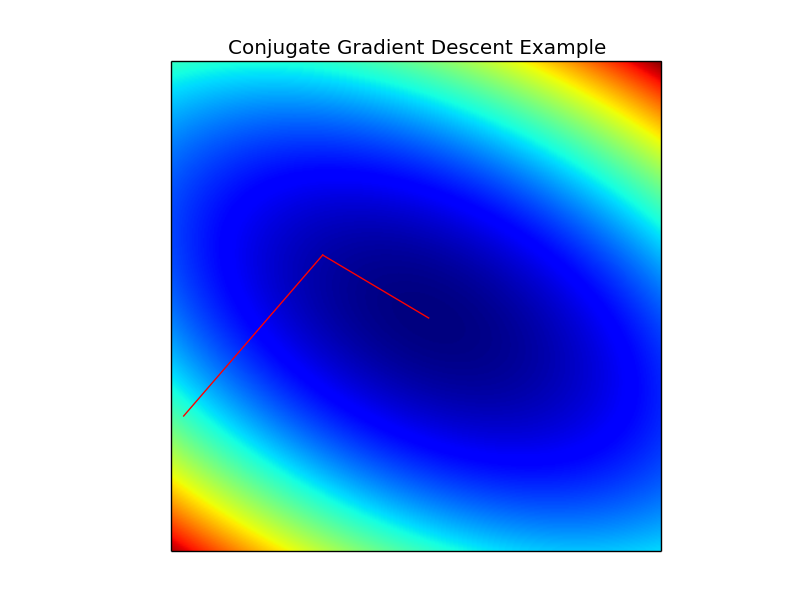
\includegraphics[scale=0.40]{CGD_example.png}\caption{CGD iterations}
\end{center}
\end{figure}


\subsection{Preconditioning}\label{precon}
In order to have a solving method with faster convergence, one can use preconditioning on the matrix $A$ and the vector $F$ so that $A$ is better conditioned. The simplest technique is to use a diagonal matrix which is the inverse of the diagonal of $A$ and so transforming the problem into solving :
\[
P=diag(A);P^{-1}x=P^{-1}F
\]
Thus in the GD and CGD the optional second argument is a vector which will multiply $A$ and the vector $F$ element-wise as if $P$ was a diagonal matrix with this vector of values. \\
Note that using the preconditioning implies changes in the matrix, thus if one wants to consecutively solve systems, one has to check the matrix values.



\subsection{Example}
Let's look at an example by solving a tridiagonal matrix given by :
\[
\left(
\begin{matrix}
2&-1&&\\
-1&2&-1&\\
&...&&\\
&&-1&2
\end{matrix}
\right)
\]
using gradient based methods (with a size of $20000\times20000$. We will first see the convergence difference between the Conjugate Gradient Descent and the Gradient Descent with and without preconditioning.
I present here some plots of the errors for the given problem given the specific solving algorithms presented before. We can clearly see the huge impact of preconditioning on the CGD and the GD. However the CGD is assured to reach the solution in at most $N$ iterations but the GD can need far more iterations to reach the stop criteria.
\begin{figure}[H]
\begin{center}
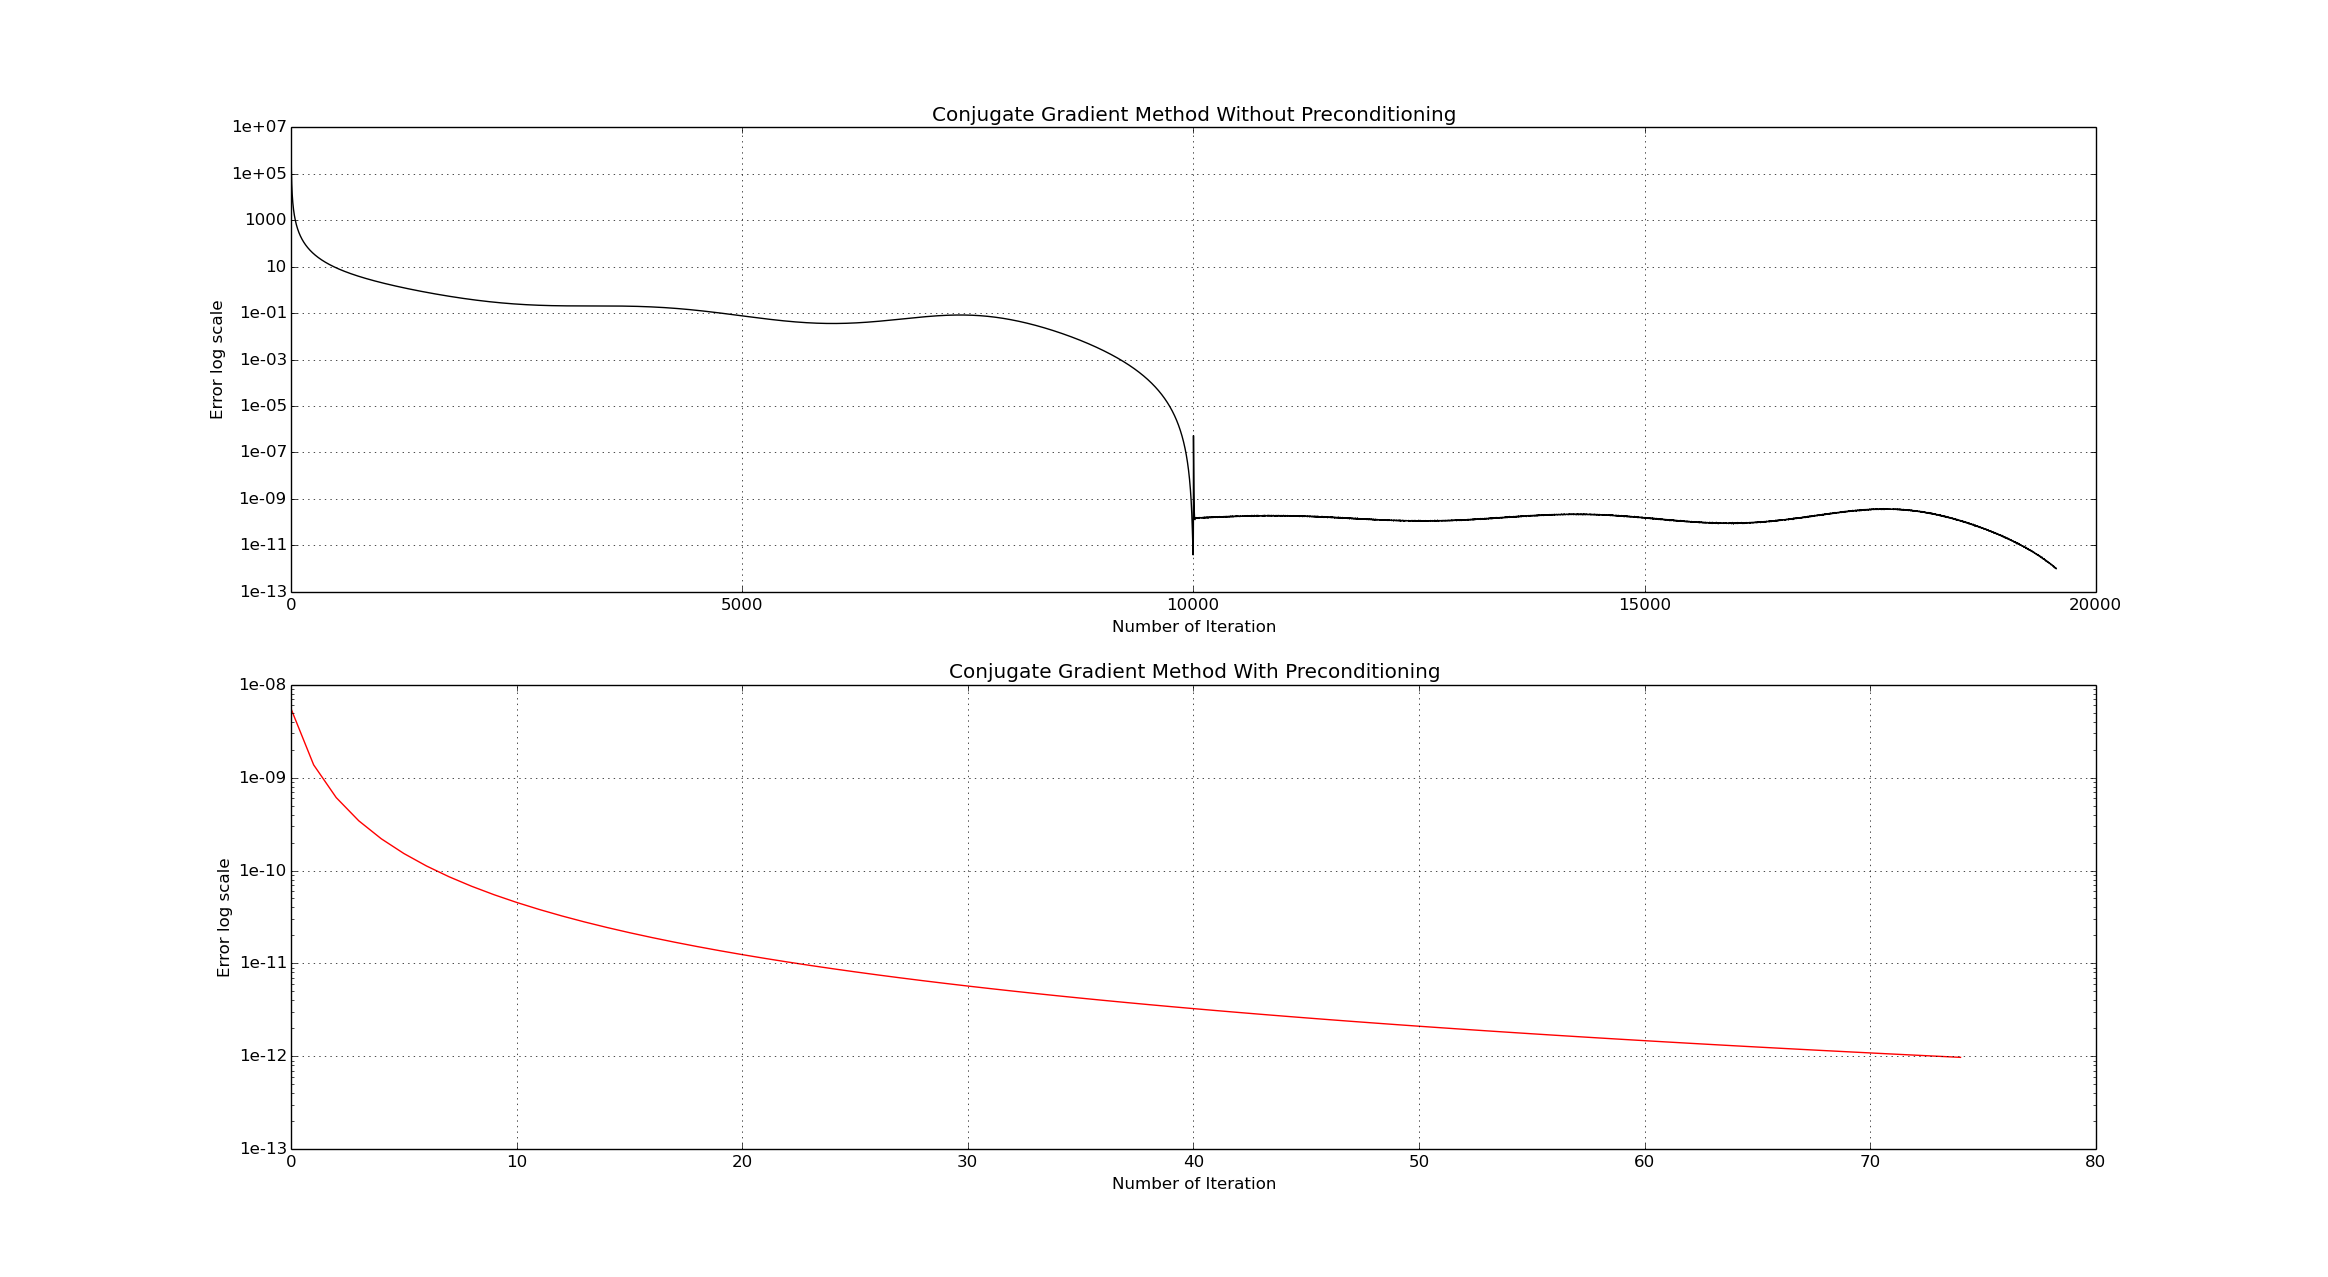
\includegraphics[scale=0.20]{cgd_error.png}\caption{Errors vs Number of iterations for the CGD with and without preconditioning, log scale for Y axis}
\end{center}
\end{figure}

\begin{figure}[H]
\begin{center}
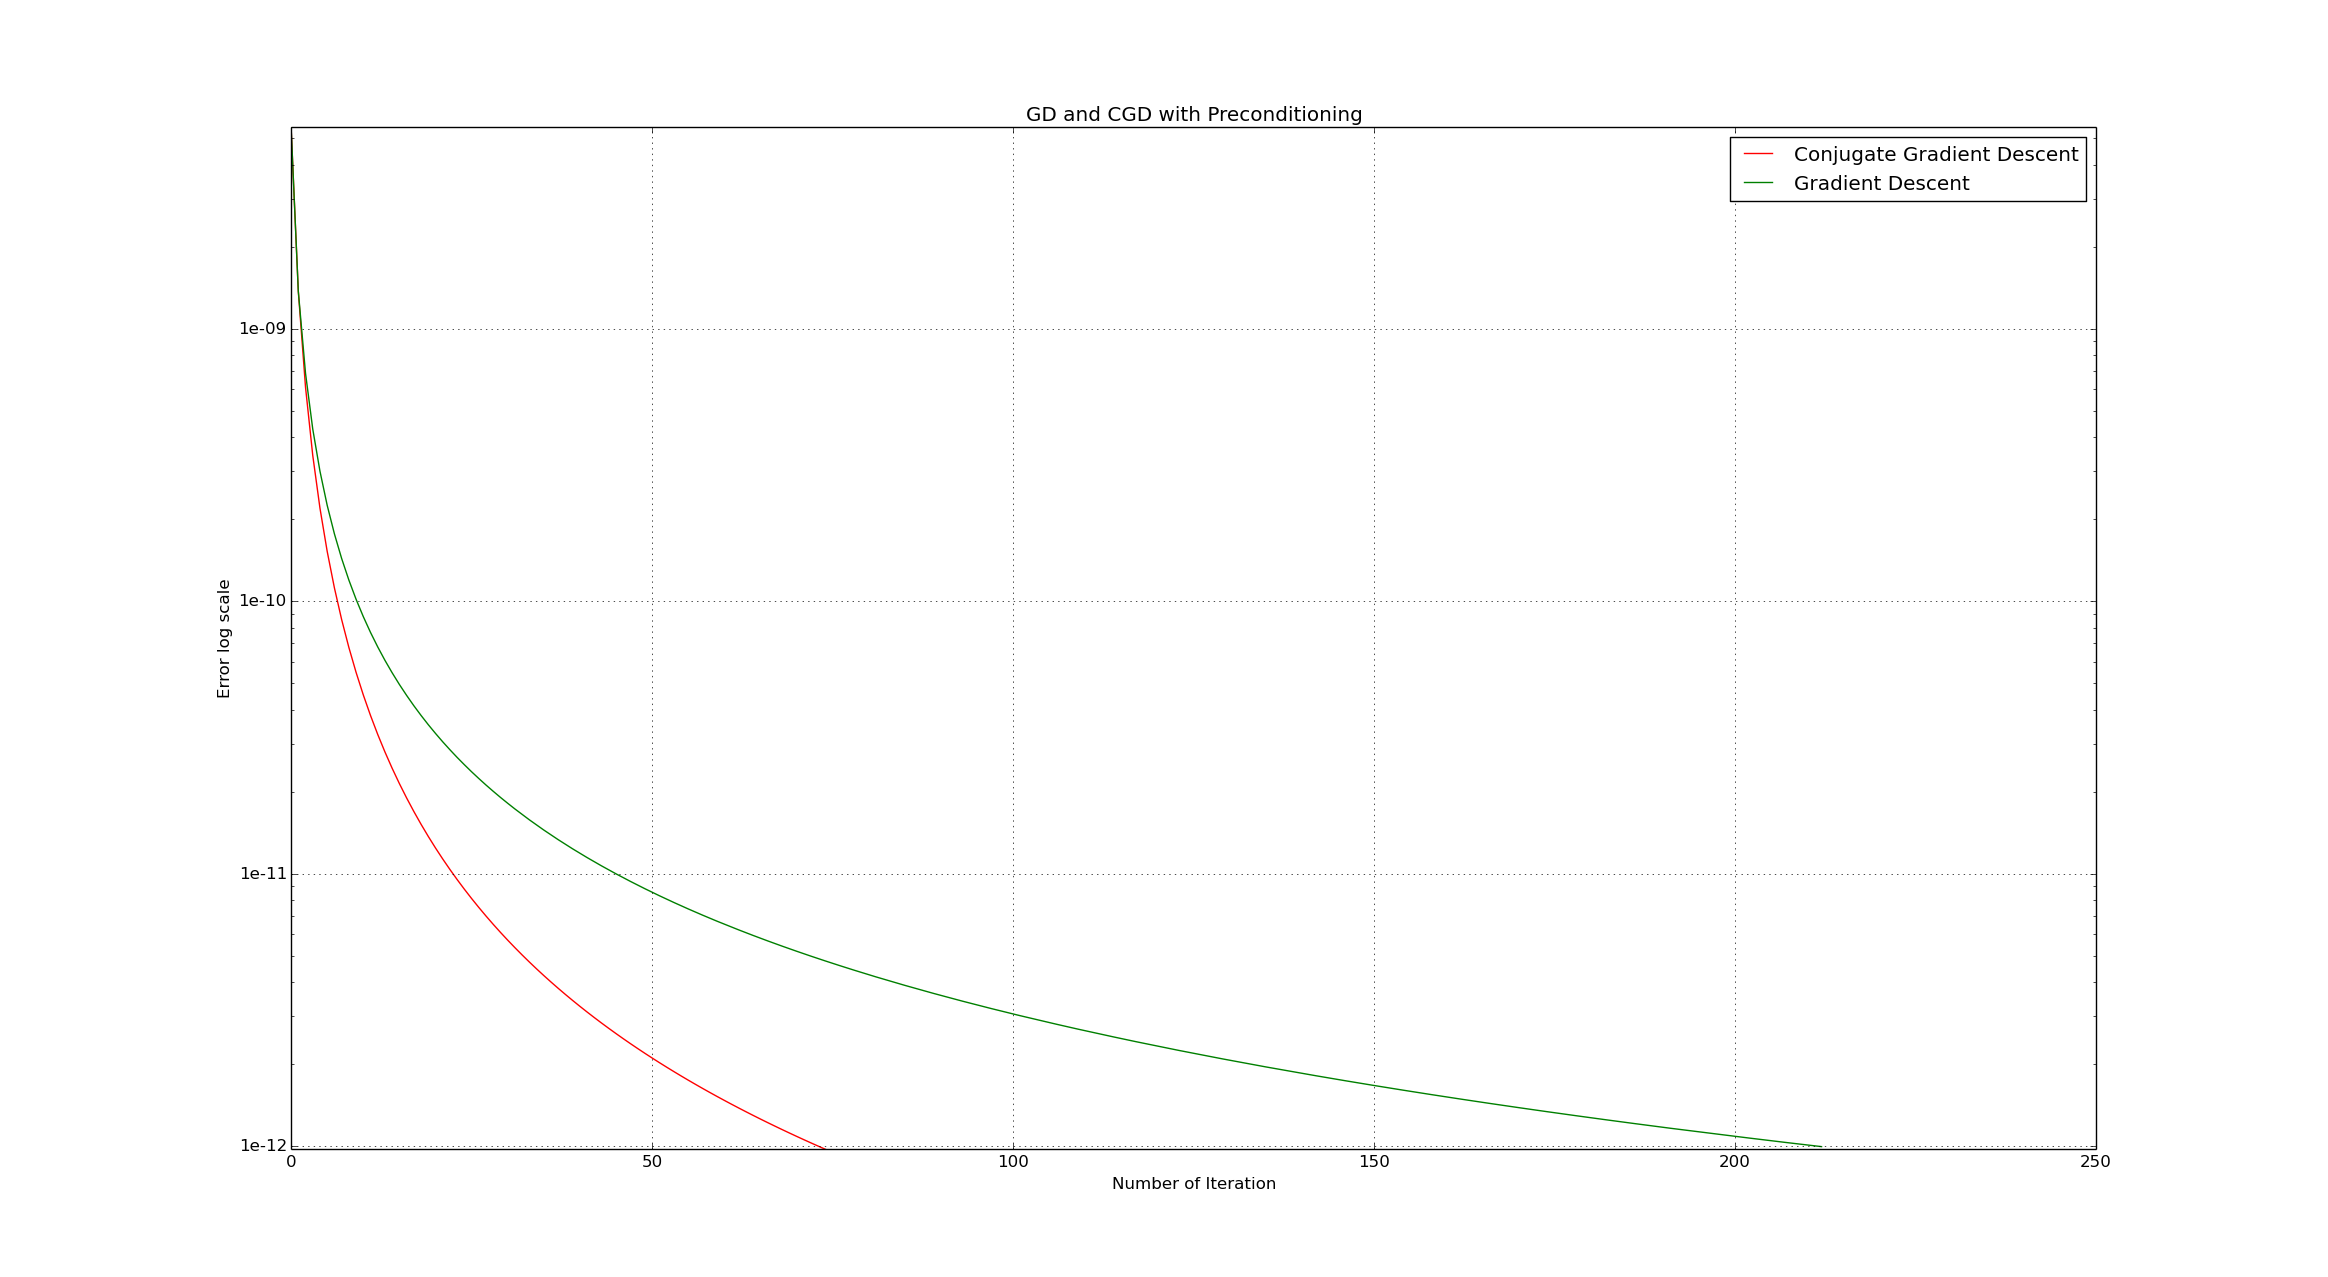
\includegraphics[scale=0.20]{cgd_gd.png}\caption{Difference between CGD and GD with preconditioning on solving the system}
\end{center}
\end{figure}
\part{Validation on a Finite Element Approximation}

\chapter{Initial Problem}
The goal is to study the heat distribution in a $2$-dimensional squared domain $\Omega$ through Laplace's equation. The domain boundary is divided into four parts ($\Sigma_1:=\{0\}\times]0,1[$, $\Sigma_2:=]0,1[ \times \{1\}$, $\Sigma_3:=\{1\} \times ]0,1[$, $ \Sigma_4:=]0,1[\times \{0\}$)  corresponding to the four sides of the domain.\\
The heat conductivity of the material on the domain is given by the function $\alpha$ which is defined by parts.\\
There are two boundary conditions : one part with a homogeneous Dirichlet condition (on the bottom side of the domain) meaning that the temperature of the material is kept to $0$ on this side; the remaining boundary has a  Neumann condition, symbolizing the heat transfer between the material and the exterior (another material for example).

\begin{itemize}
\item The Initial Problem (PI) : 
\begin{equation}\label{eq:1}
\left\{
\begin{array}{l}
\text{Find $u\in H^2_D(\Omega)$ such that}\\
-\alpha \Delta u = 0 \text{ on $\Omega$ with $\alpha \in L^\infty (\Omega)$}\\
\frac{\partial u}{\partial n}=g \text{ on $\Gamma_N:=\Sigma_1 \cup \Sigma_2 \cup \Sigma_3$ with $g\in L^\infty (\Gamma_N)$}\\
u=0 \text{ on $\Gamma_D := \Sigma_4$}
\end{array}
\right.
\end{equation}

Where $H^2_D(\Omega):=\{ v \in H^2(\Omega) : v|_{\Gamma_D}=0\}$ with $.|_{\Gamma_D}$ being the trace operator.
\item 
The function $g$ defined on $\Gamma_N$ with $g_i : \mathbb{R} \rightarrow \mathbb{R} ,i=1,2,3$ :
\begin{align*}
g:\Gamma_N \subset \mathbb{R}^2 &\rightarrow \mathbb{R} \\
(x,y)&\rightarrow \left\{
\begin{array}{l}
g_1(y), \text{ if }(x,y) \in \Sigma_1\\
g_2(x),\text{ if }(x,y) \in \Sigma_2\\
g_3(y),\text{ if }(x,y) \in \Sigma_3\\
\end{array}
\right.
\end{align*}
\item The function $\alpha$ defined on $\Omega$ with $\alpha_i : \mathbb{R} \rightarrow \mathbb{R} ,i=1,...,9$ : 
\begin{align*}
\alpha:\Omega \subset \mathbb{R}^2 &\rightarrow \mathbb{R} \\
(x,y)&\rightarrow
\alpha_i(x,y), \text{ if }(x,y) \in \Omega_i, i=1,...,9
\end{align*}


\end{itemize}

\begin{figure}[H]
\begin{center}
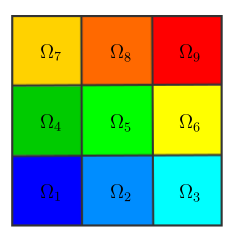
\includegraphics[scale=0.40]{subdomain.png}\caption{Sub-domains corresponding to $\Omega_i$ representing the different conductivity levels.}
\end{center}
\end{figure}


\chapter{Variational Problem}
\section{Weak Form Derivation}
We will now derive the variational formulation of the initial problem \ref{eq:1}


\begin{align*}
&\forall v \in H^1_D(\Omega)\\
&\int_\Omega (- \alpha \Delta u)v dxdy=0\\
\implies & - \int_{\partial \Omega} (\alpha|_{\partial \Omega} \nabla u.\overrightarrow{n}) v|_{\partial \Omega}  d \sigma+
\int_\Omega (\alpha \nabla u).(\nabla v)dxdy=0
\text{ (Green)}
\\
\implies & - \int_{\Gamma_N} \alpha|_{\Gamma_N} \frac{\partial u}{\partial n}v|_{\Gamma_N}  d\sigma-
 \int_{\Gamma_D} \alpha|_{\Gamma_D} \frac{\partial u}{\partial n}v|_{\Gamma_D}d \sigma +\int_\Omega (\alpha\nabla u).(\nabla v)dxdy=0\\
 \implies & \int_\Omega (\alpha\nabla u).(\nabla v)dxdy =\int_{\Gamma_N} \alpha|_{\Gamma_N}gv|_{\Gamma_N} d\sigma \text{ (Boundary Conditions)}
\end{align*}
Leading to the variational problem
\begin{equation}\label{eq:2}
\left\{
\begin{array}{l}
\text{Find u $\in H^1_D(\Omega)$ such that}\\
a(u,v)=l(v), \forall v \in H^1_D(\Omega)
\end{array}
\right.
\end{equation}
We now have \ref{eq:1}$\implies $\ref{eq:2} with :
\[
a(u,v):=\int_\Omega (\alpha\nabla u).(\nabla v)dxdy
\]
\[
l(v):=\int_{\Gamma_N} \alpha |_{\Gamma_N}gv|_{\Gamma_N} d\sigma
\]
\section{Problem Equivalence}
We will now check that \ref{eq:2}$\implies$\ref{eq:1} assuming that $u \in H^2(\Omega)$\\
\begin{align*}
&\forall \phi \in \mathcal{D}(\Omega)\subset H^1_D(\Omega),\\
&\int_\Omega (\alpha \nabla u).(\nabla \phi) dxdy=\int_{\Gamma_N} \alpha |_{\Gamma_N}g \phi |_{\Gamma_N} d\sigma\\
\implies & \int_\Omega (\alpha \nabla u).(\nabla \phi) dxdy=0\text{ (Compact Support of $\phi$}\\
\implies & \int_{\partial \Omega} (\alpha \nabla u . \overrightarrow{n})\phi |_{\partial \Omega} d\sigma - \int_\Omega \alpha \Delta u \phi dxdy=0\\
\implies &- \int_\Omega \alpha \Delta u \phi dxdy=0, \forall \phi \in \mathcal{D}(\Omega)\\
\implies & - \alpha \Delta u =0 \text{ almost everywhere on } \Omega
\end{align*}
Let's find the Neumann boundary condition (the Dirichlet condition is already included into $H^1_D(\Omega)$) :
\begin{align*}
&\forall v \in H^1_D(\Omega),\\
&\int_\Omega (\alpha \nabla u).(\nabla v) dxdy=\int_{\Gamma_N}\alpha |_{\Gamma_N}g v |_{\Gamma_N} d\sigma\\
\implies & \int_{\partial \Omega} (\alpha|_{\partial \Omega} \nabla u .\overrightarrow{n}) v|_{\partial \Omega} d\sigma - \int_\Omega (\alpha \Delta u ) v dxdy = \int_{\Gamma_N}\alpha|_{\Gamma_N}g v |_{\Gamma_N} d\sigma\\
\implies & \int_{\Gamma_N} \alpha|_{\Gamma_N} \nabla u .\overrightarrow{n}v|_{\Gamma_N} d\sigma = \int_{\Gamma_N}\alpha |_{\Gamma_N}g v |_{\Gamma_N} d\sigma, \forall v \in H^1_D \\
\implies & \frac{\partial u}{•\partial n}=g \text{ on } \Gamma_N
\end{align*}
Thus we have : $\ref{eq:1} \iff \ref{eq:2}$
\section{Existence and Uniqueness of the Solution}
We will now prove the uniqueness of the solution through the Lax-Milgram's Theorem :
\begin{itemize}
\item $H^1_D(\Omega)$ is a Hilbert space with the scalar product $<.,.>_{H^1(\Omega)}$. In fact, $H^1_D(\Omega):=ker(.|_{\Gamma_D})$. Since the trace operator is a linear and continuous operator, $H^1_D(\Omega)$ is closed. In addition, $H_D^1(\Omega) \subset H^1(\Omega)$ thus $H^1_D(\Omega)$ is a Hilbert space.
\item $a$ and $l$ are bilinear and linear respectively by definition of the integral.
\item $l$ is continuous :
\begin{align*}
&\forall v\in H^1_D(\Omega):\\
&|l(v)|\leq ||\alpha|_{\Gamma_N} ||_{L^\infty(\Gamma_N)}||g||_{L^2(\Gamma_N)}||v|_{\Gamma_N}||_{L^2(\Gamma_N)}\\
&|l(v)| \leq ||\alpha|_{\Gamma_N}||_{L^\infty(\Gamma_N)} ||g||_{L^2(\Gamma_N)} K ||v||_{H^1(\Omega)}\\
&|l(v)| \leq C ||v||_{H^1(\Omega)}
\end{align*}
With $K$ being the continuity constant of the trace operator :
\[
||u|_\Gamma||_{L^2(\Gamma)} \leq K ||u||_{H^1(\Omega)}
\]
\item $a$ is continuous :
\begin{align*}
&\forall u,v \in H^1_D(\Omega):\\
&|a(u,v)|\leq  ||a||_{L^\infty(\Omega)} || \nabla u||_{L^2(\Omega)} || \nabla v||_{L^2(\Omega)}\\
&|a(u,v)| \leq  ||a||_{L^\infty(\Omega)} ||u||_{H^1(\Omega)} ||v||_{H^1(\Omega)}\\
&|a(u,v)| \leq C || u||_{H^1(\Omega)} || v||_{H^1(\Omega)}
\end{align*}
\item $a$ is coercive, if we require $\alpha \geq \alpha_0 > 0$ :
\begin{align*}
& \forall u \in H^1_D(\Omega):\\
&a(u,u)=\int_\Omega \alpha |\nabla u|^2dxdy\\
&a(u,u) \geq \alpha_0 ||\nabla u||^2_{L^2(\Omega)}\\
&a(u,u) \geq \frac{\alpha_0}{1+C^2_P} ||u||^2_{H^1(\Omega)}\\
&a(u,u) \geq C ||u||^2_{H^1(\Omega)}
\end{align*}
Thus using Poincare's inequality leads to the coercivity through the condition $\alpha >0$
which is not a problem since in our case $\alpha$ stands for the heat conductivity of the material.
Note that we can use the Poincare's inequality  because of the Dirichlet condition :
\[
||f||_{L^2(\Omega)} \leq C_p ||\nabla f||_{L^2(\Omega)}
\]
Thus we can derive :
\begin{align*}
||u||_{H^1(\Omega)}^2&=||u||_{L^2(\Omega)}^2+||\nabla u ||_{L^2(\Omega)}^2\\
&\leq C_p^2||\nabla u ||^2_{L^2(\Omega)}+||\nabla u ||^2_{L^2(\Omega)}\\
&\leq (1+C_p^2)||\nabla u ||_{L^2(\Omega)}\\
||u||_{H^1(\Omega)}^2\frac{1}{(1+C_p^2)}&\leq ||\nabla u ||^2_{L^2(\Omega)}
\end{align*}
\end{itemize}
Therefore all the conditions for the Lax-Milgram's Theorem are checked, we thus have :
\[
\exists ! u \in H^1_D(\Omega) : a(u,v)=l(v), \forall v \in H^1_D(\Omega)
\]

\chapter{Discretized Problem}
\section{Existence and Uniqueness of the Solution}
We will use the Galerkin method in order to discretize the problem and solve it.
Given a triangulation of $\Omega$, we define :
\begin{itemize}
\item $P^1$ is the set of all the degree one polynomials ($a+bx+cy$).
\item $v|_{T_i}$ will be the restriction of $v$ on the $i^{th}$ triangle.
\item $
V_h(\Omega):=\{ v_h \in C^0(\bar{\Omega}) : v_h|_{T_i} \in P^1(T_i),v_h|_{\Gamma_D}=0\}
$
\item $V_h(\Omega) \subset V(\Omega):=H^1_D(\Omega)$
\end{itemize}

Since we know that :
\begin{itemize}
\item $V_h(\Omega)$ is a finite dimension space, thus is closed
\item $V_h(\Omega) \subset H^1_D(\Omega)$
\end{itemize}
we can use again the Lax Milgram's theorem giving the existence and uniqueness of the solution to the discretized problem with \ref{eq:3}$\iff$\ref{eq:2}.

\begin{equation}\label{eq:3}
\left\{
\begin{array}{l}
\text{Find $u_h \in V_h$ such that}\\
a(u_h,v_h)=l(v_h), \forall v_h \in V_h
\end{array}
\right.
\end{equation}

\section{Mesh Description}
Given a discretization of the domain into a $2D$ mesh with nodes $x_{i}$ (note necessarily equidistant) the degrees of freedom are $\{ x_{i} \in \Omega : x_{i} \not\in \Gamma_D \}$.
In the specific case of a uniform mesh and with
\begin{itemize}
\item $\Omega=[0,1]^2$
\item $N$ points in $x$, $h_x=\frac{1}{N-1}$ 
\item $M$ points in $y$, $h_y=\frac{1}{M-1}$
\item dim($V_h$) = $MN-N$ because of the Dirichlet condition
\item $x_i=((i\mod N)h_x,floor(i/N)h_y),0\leq i\leq MN-1$
\end{itemize} 


Thus leading to the following node labelling where we list the nodes $x_i$ from left to right and from bottom to top.

\begin{center}
\begin{tabular}{cccc}
$x_{(M-1)N}$ &$ x_{(M-1)N +1}$ & ... &$x_{MN-1}$\\
& ...& &\\
$x_N $& $x_{N+1}$ & ... &$x_{2N-1}$\\
$x_0$ &$ x_1$ &... &$x_{N-1}$
\end{tabular}
\end{center}

Here is a  little mesh example with $N=M=3$ :
\begin{figure}[H]
\begin{center}
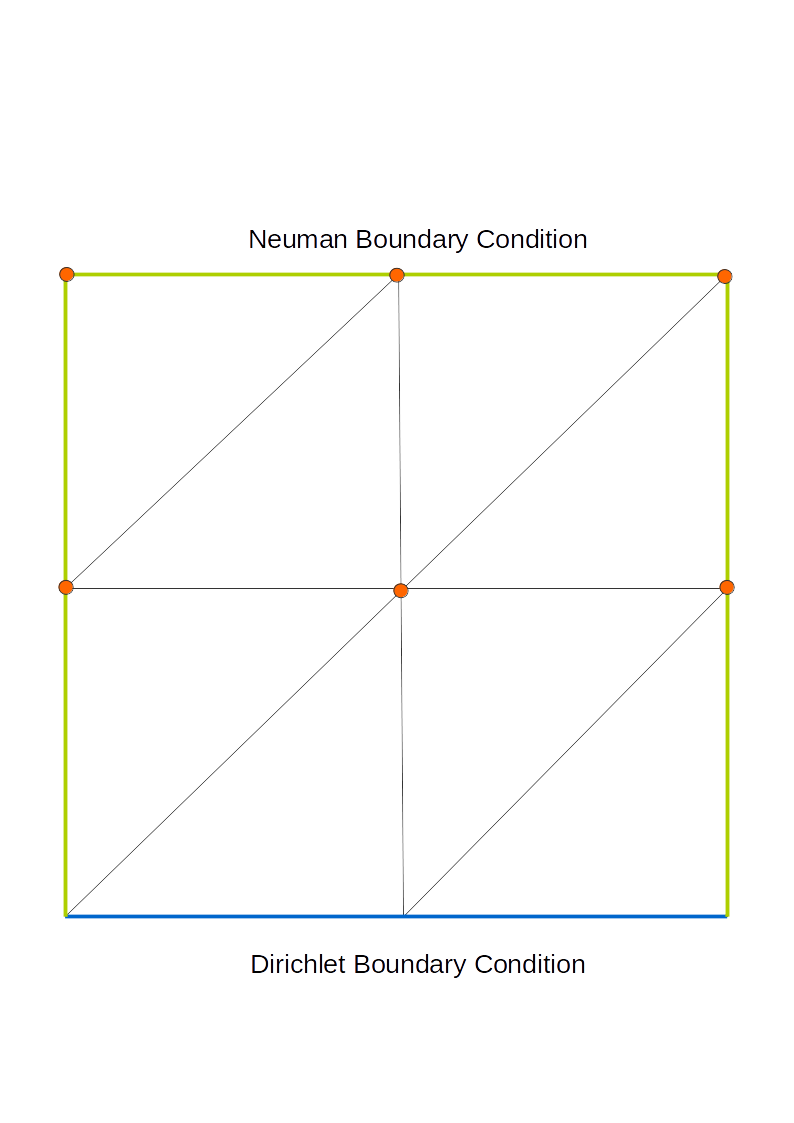
\includegraphics[scale=0.30]{mesh.png}\caption{Mesh example, Orange : degrees of freedom}
\end{center}
\end{figure}

We use a uniform mesh but the used algorithms are not specialized. Each node needs a label in order to know if it belongs to the boundary or not. We also assume the Dirichlet condition.
The labels are necessary for example to know if a triangle belongs to the boundary (to know how many of its three defining points belong to the boundary) for the linear form computation.


Since we will use $P^1$ Lagrange polynomials, 
the basis functions are the hat functions $w^{i}$ with
\[
w^{(i)}(x_{k})= \delta_{ik} =  \left\{
\begin{matrix}
1,\text{if $i=k$} \\
0,\text{otherwise}\\
i,k \in \{N,...,NM-1\}
\end{matrix}
\right.
\]
Those functions form a basis of $V_h(\Omega)$, in fact
\begin{itemize}
\item $w^{(i)} \in V_h(\Omega),\forall i$
\item $|\{ w^{(i)},i=N,...,NM-1 \} |=(M-1)N=dim(V_h)$
\item $(w^{(i)})_{i=N}^{NM-1}$ are linearly independent.
\end{itemize}
We just need to show that they are linearly independent :
\begin{align*}
&\sum_{i=N}^{NM-1} w^{(i)}(x,y)\lambda_{i}=0\\
\implies & \sum_{i=N}^{NM-1} w^{(i)}(x_k)\lambda_{i}=0,\forall k \in \{N,...,NM-1 \}\\
\implies & \lambda_{i}=0,\forall i
\end{align*}

\section{System $Au=L$}
We will now see how this discretized problem can be solved using a linear system. We already know that : 
\[
\exists ! u_h \in V_h(\Omega) : a(u_h,v_h)=l(v_h), \forall v_h \in V_h(\Omega)
\]
This implies directly that 
\[
\exists ! u_h \in V_h(\Omega) : a(u_h,w^{(i)})=l(w^{(i)}), \forall i \in \{ N,...,NM-1\}
\]
Now by using the fact that we have a basis for $V_h(\Omega)$ we can rewrite any function as a linear combination of this basis leading to $u_h=\sum_{i=N}^{NM-1} u_h(x_i)w^{(i)}$.
\\
Now by using the bilinearity of $a$ we have :
\begin{align*}
&a(u_h,w^{(i)})=l(w^{(i)}), \forall i \in \{ N,...,NM-1\}\\
\implies & a(\sum_{j=N}^{NM-1} u_h(x_j)w^{(j)},w^{(i)})=l(w^{(i)}), \forall i \in \{ N,...,NM-1\}\\
\implies & \sum_{j=N}^{NM-1} u_h(x_j)a(w^{(j)},w^{(i)})=l(w^{(i)}), \forall i \in \{ N,...,NM-1\}\\
 \implies & Au=L
\end{align*}
With 
\[
A=\left(\begin{matrix}
a(w^{(N)},w^{(N)}) & a(w^{(N+1)},w^{(N)}) & ... & a(w^{(NM-1)},w^{(N)})\\
a(w^{(N)},w^{(N+1)}) & a(w^{(N+1)},w^{(N+1)}) & ... & a(w^{(NM-1)},w^{(N+1)})\\
 & &...&\\
a(w^{(N)},w^{(NM-1)}) & a(w^{(N+1)},w^{(NM-1)}) & ... & a(w^{(NM-1)},w^{(NM-1)})
\end{matrix} \right)
\]
\[
u=\left( 
\begin{matrix}
u_h(x_N)\\
u_h(x_{N+1})\\
...\\
u_h(x_{NM-1}) 
\end{matrix}\right) 
,
L=\left( 
\begin{matrix}
 l(w^{(N)})\\
 l(w^{(N+1)})\\
...\\
 l(w^{(NM-1)})\\  
 \end{matrix}\right)
\]


Thus we end up by simply having a linear system to solve of size $N(M-1)\times N(M-1)$ but we will see that the matrix $A$ is sparse.
\chapter{Discretized Problem Computation}
\section{Quadrature}
\subsection{Triangle Area}
In order to quickly compute the area of a triangle ($T_k$) given its three nodes, we use the following formula :
\[
area(T_k)=\frac{| (y_3-y_1)(x_2-x_1)-(y_2-y_1)(x_3-x_1) |}{2}
\]
In fact, if we have three points in a $2D$ space (defining the triangle) the determinant of the matrix
\[
\left(
\begin{matrix}
x_1 & y_1 & 1\\
x_2 & y_2 & 1\\
x_3 & y_3 & 1\\
\end{matrix}
\right)
\]
divided by $2$ will give us the (signed) area of the triangle, thus we take the absolute value.
\subsection{Hat Functions}
By the nature of the basis functions ($w^{(i)}$), also called the "hat" functions because of their shape, we have some properties : 
\begin{itemize}
\item $w^{(i)}|_{T_i} \in P^1(T_i),\forall i$ 
\item $\nabla w^{(i)}|_{T_i} \in P^0(T_i), \forall i$
\item $w^{(i)}(x,y) =0$ and thus $\nabla w^{(i)}(x,y)=0$ if $(x,y) \not \in $ adjacent triangles of $x_i$ 
\end{itemize}
Let's compute the explicit expression of $w^{(i)}$ on any triangle $T_k$ adjacent to $x_{i}$ since otherwise $w^{(i)}=0$. We know that  $w^{(i)}(x_{i})=1$ and that a triangle is defined by its three nodes (where one of them is $x_i$) $(x_1,y_1,z_1),(x_2,y_2,z_2),(x_3,y_3,z_3)$. We will thus compute the plane equation given its normal vector and one of the points.
\\
The two vectors computed from the triangles are
\[
\left(
\begin{matrix}
x_2-x_1\\
y_2-y_1\\
z_2-z_1\\
\end{matrix}
\right),
\left(
\begin{matrix}
x_3-x_1\\
y_3-y_1\\
z_3-z_1\\
\end{matrix}
\right)
\]
We now compute the cross product by finding the determinant of the following matrix
\[
\left(
\begin{matrix}
i & j & k\\
x_2-x_1&y_2-y_1&z_2-z_1\\
x_3-x_1&y_3-y_1&z_3-z_1
\end{matrix}
\right)
\]
Leading to the normal vector :
\[
\left(
\begin{matrix}
(y_2-y_1)(z_3-z_1)-(z_2-z_1)(y_3-y_1)\\
-(x_2-x_1)(z_3-z_1)+(z_2-z_1)(x_3-x_1)\\
(x_2-x_1)(y_3-y_1)-(y_2-y_1)(x_3-x_1)
\end{matrix}
\right):=
\left(
\begin{matrix}
a_1\\
a_2\\
a_3
\end{matrix}
\right)
\]
Thus the equation of the plane is of the form
\[
a_1x+a_2y+a_3z=d
\] where $d$ is determined by plugging in one of the three nodes leading to the formula
\[
\forall (x,y) \in T_k \subset supp(w^{(i)}),w^{(i)}(x,y)=\frac{- a_1x-a_2y+ (a_1x_i+a_2y_i+a_3z_i)  }{a_3}
\]
With $T_k$ being a triangle having $x_i$ as one of its node.
This allows us to compute explicitly the gradient :
\[
\forall (x,y) \in T_k \subset supp(w^{(i)}),\nabla w^{(i)}(x,y)=\left(
\begin{matrix}
\frac{-a_1}{a_3}\\
\frac{-a_2}{a_3}
\end{matrix}
\right)
:=
\left(
\begin{matrix}
g^i_{1,k}\\
g^i_{2,k}
\end{matrix}
\right)
\]
\section{Bilinear Form Computation}
We will now investigate the bilinear form which will be used to fill the matrix $A$. We will denote by $T_k[i],i=1,2,3$ the node $i$ of the triangle $k$. 
\begin{align*}
a(w^{(i)},w^{(j)})=&\int_\Omega (\alpha \nabla w^{(i)}).(\nabla w^{(j)})dxdy\\
=&\sum_{k=0}^{K-1}\int_{T_k} \alpha(\nabla w^{(i)}.\nabla w^{(j)})dxdy\\
=&\sum_{k=0}^{K-1} (g_{1,k}^ig_{1,k}^j+g_{2,k}^ig_{2,k}^j) \int_{T_k} \alpha dxdy\\
=&\sum_{k=0}^{K-1} (g_{1,k}^ig_{1,k}^j+g_{2,k}^ig_{2,k}^j)*\frac{\alpha(T_k[0])+\alpha(T_k[1])+\alpha (T_k[2])}{3}*area(T_k)
\end{align*}
If $x_i$ and $x_j$ are not nodes of the triangle $T_k$ it is equal to $0$. Note that the last approximation is actually an exact quadrature except if $T_k$ belongs to two different sub-domains $\Omega_i$. 
So we will loop over the triangles to fill $A$ and add the new computed contribution to the right position. Note that since $\alpha$ is constant on each $\Omega_i$ we could have used a faster quadrature formula by simply using the middle point for example. However, in a case where we have triangles on two sub-domains, this quadrature reduces the error.\\
In the particular case of a uniform mesh, the matrix will be tridiagonal by tridiagonal blocks.
\section{Linear Form Computation}
\[
l(w^{(i)})=\int_{\Gamma_N} \alpha |_{\Gamma_N} g w^{(i)}|_{\Gamma_N} d \sigma
\]
For most of the $w^{(i)}$ functions, we will have $l(w^{(i)})=0$. But we can efficiently compute it knowing that this will be non-zero if and only if $x_i \in \Gamma_N$. We can already say that 
\begin{align*}
x_i \in \Gamma_N \iff i \in & \{N,2N,...,(M-1)N,\\
&(M-1)N+1,..., NM-1,\\
   &(M-1)N-1,(M-2)N-1,...,2N-1\}:= X
\end{align*}
We can even see that by looking only at the nodes on the boundary, the node $x_{X[s]}$ has two adjacent nodes in $X$ : 
$x_{X[s-1]}$ and $x_{X [s+1]}$ with $s=1,...,2M+N-5$ in fact $|X | =2M+N-4 $.
And so we can see that if $i\in X$ we will need to compute the area under two segments to compute $l(w^{(i)})$.
We then have the following formula if we note $w^{\left(X[i]\right)}:=w$ and we assume $h_y=h_x=h$ for convenience (otherwise we need to distinguish the case $x_{X[i]} \in \Sigma_1 \cup \Sigma_3$ from $x_{X[i]} \in \Sigma_2 $) :
\begin{align*}
l\left(w\right)=&h*\frac{\alpha(x_{X[i-1]})*g(x_{X[i-1]})*
w(x_{X[i-1]})+\alpha(x_{X[i]})*g(x_{X[i]})*w(x_{X[i]})}{2}+\\
&h*\frac{\alpha(x_{X[i+1]})*g(x_{X[i+1]})*
w(x_{X[i+1]})+\alpha(x_{X[i]})*g(x_{X[i]})*w(x_{X[i]})}{2}\\
=&h*\frac{\alpha(x_{X[i]})*g(x_{X[i]})*w(x_{X[i]})}{2}+h*\frac{\alpha(x_{X[i]})*g(x_{X[i]})*w(x_{X[i]})}{2}\\
=&h*\alpha(x_{X[i]})*g(x_{X[i]})*w(x_{X[i]})
\end{align*}
By using the fact that $w(x_{X[k]})=\delta_{X[i]X[k]}$. Since on each $\Omega_i \cap \Gamma_N$ we have $\alpha \in P^0$, $g \in P^0$, $w^{(i)}\in P^1$ the used quadrature formula is exact. This would not be the case without these properties.  Let's look at an example with the $3 \times 3$ mesh and with $w^{(3)}|_{\partial \Omega}$
\begin{figure}[H]
\begin{center}
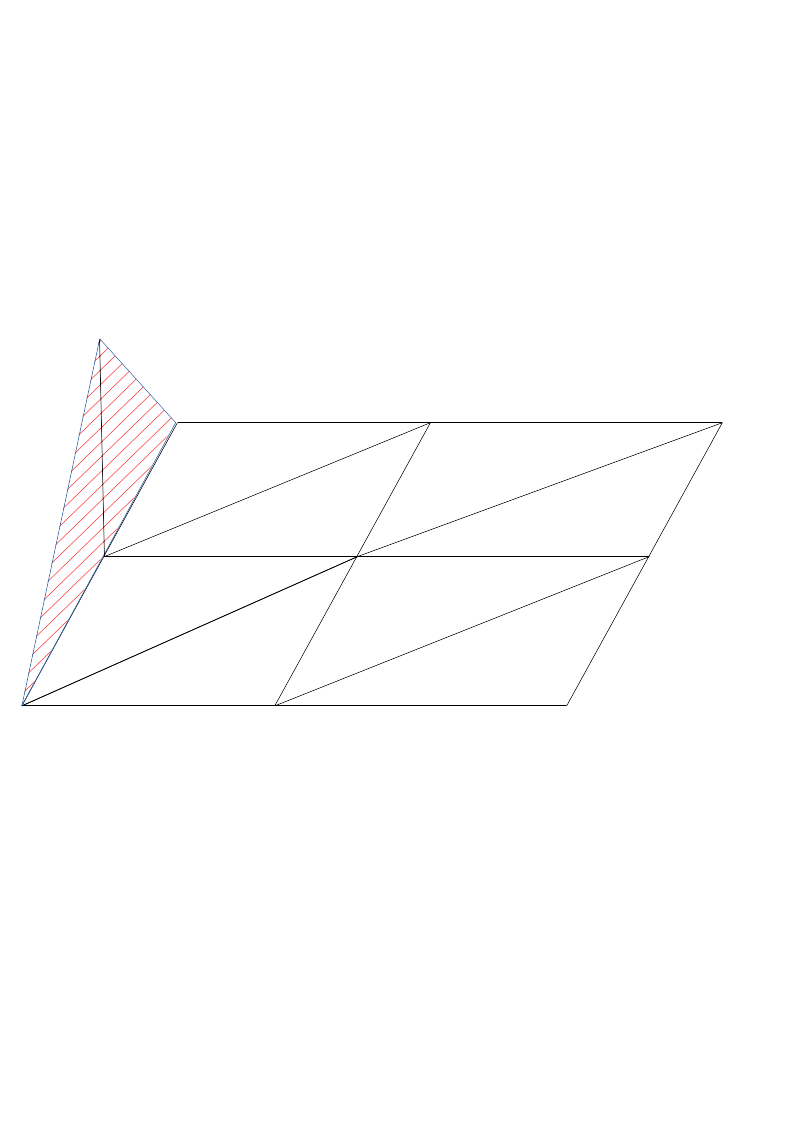
\includegraphics[scale=0.30]{li.png}\caption{Example of  $w^{(3)}|_{\Gamma_N}$ }
\end{center}
\end{figure}
\section{Implementation of Piecewise-Defined Functions}
\subsection{$\alpha$ function}
First of all, we have the function $\alpha$ which is defined by parts with the functions $\alpha_i : \Omega_i \subset \mathbb{R}^2 \rightarrow \mathbb{R}$. This comes from the heat conductivity of the material which is not constant on the whole domain. This is for example the case if the studied material is actually itself a composite of some pieces each having different properties. In order to keep a general approach to this, we define a special class $alpha$ which will hold all the sub-domains and the corresponding values. Then, when we use the access operator, for a specific $\mathbb{R}^2$ point, a special method will find to which sub-domain this point belongs to and then will return the right value. Here is an example : 
\begin{lstlisting}[basicstyle=\tiny]
    alpha al;
    al.AddDomain(0,0,0.3,0.5,1);
    al.AddDomain(0.3,0,0.6,0.5,6);
    al.AddDomain(0.6,0,1,0.5,1);
    al.AddDomain(0,0.5,1,1,1);
    al(0.2,0.2);
\end{lstlisting}
Note that the domains are rectangular domains defined by the two extreme points and the corresponding return value. A generalisation for every shape is possible but then in order to check to which sub-domain a specific point belongs to we will need a more complex method. A default constructor will automatically set the coefficients and the sub-domains as given in the studied problem.
\subsection{$g$ function}
Another function which is defined by parts is the function $g$. This function represents the heat flow coming in or out (depending on the sign of the value) the boundary of the material (except on $[0,1] \times \{0\}$ where the temperature is kept at $0$. This function is defined by a specific $g_i : \mathbb{R} \rightarrow \mathbb{R}$ function for each side of $\Omega$ (except on $\Gamma_D$). In order to have a simple class for this function, we just store the three possible values (one for each side) and then when a point is requested, a simple condition will return the right value. \\
Note that it would be possible to generalize this to any given case (for example a non constant function $g_i$) by storing the function pointer and returning the specific function return value instead of simply returning the stored value.
\section{Method to Fill the System $Au=L$}
\subsection{Optimized Approach}
Since we already know that $A$ will be sparse by the structure of the mesh we can avoid doing an algorithm of the form :
\\
\\
\begin{algorithm}[H]
 \KwData{Matrix, Vector}
 \KwResult{A filled}
 \For{i=N $\rightarrow$ NM-1}{
  \For{j=0 $\rightarrow$ NM-1}{
  	$A(i,j)=a(w^{(i)},w^{(j)})$
     }
  }
 \caption{Filling the matrix $A$ in $O(NM^2)$}
\end{algorithm}

Another approach is by computing the value of $a$ on each triangle and then add the result to the right entry of the matrix $A$. Note that by doing this it is also possible to fill the vector $L$ at the same time.

\begin{algorithm}[H]
 \KwData{Matrix, Vector}
 \KwResult{A and L filled}
 \For{k=0 $\rightarrow$ K-1}{
  \For{i=0 $\rightarrow$ 2}{
      \If{$Triangle[k][i]-N\geq 0$}{
  $L[Triangle[k][i]-N]+=b(Triangle[k],i,al,g)$\;
            \For{j=0 $\rightarrow$ 2}{
                \If{$Triangle[k][j]-N\geq 0 $}{
        $A(T[k][i]-N,T[k][j]-N)+=a(Triangle[k],i,j,al)$
                }
            }
        }
     }
  }
 \caption{Filling the matrix $A$ in $O(K)$ (about $9*K$ loops)}
\end{algorithm}
Let's see the resulting matrix for two different mesh structures to show the special "tridiagonal by tridiagonal blocks" structure defined as :
\[
\left(
\begin{matrix}
B&I&&\\
I&B&I&\\
&&...\\
&&I&B
\end{matrix}
\right)
\]
with $B$ being once again a tridiagonal matrix.
\begin{figure}[H]
\begin{center}
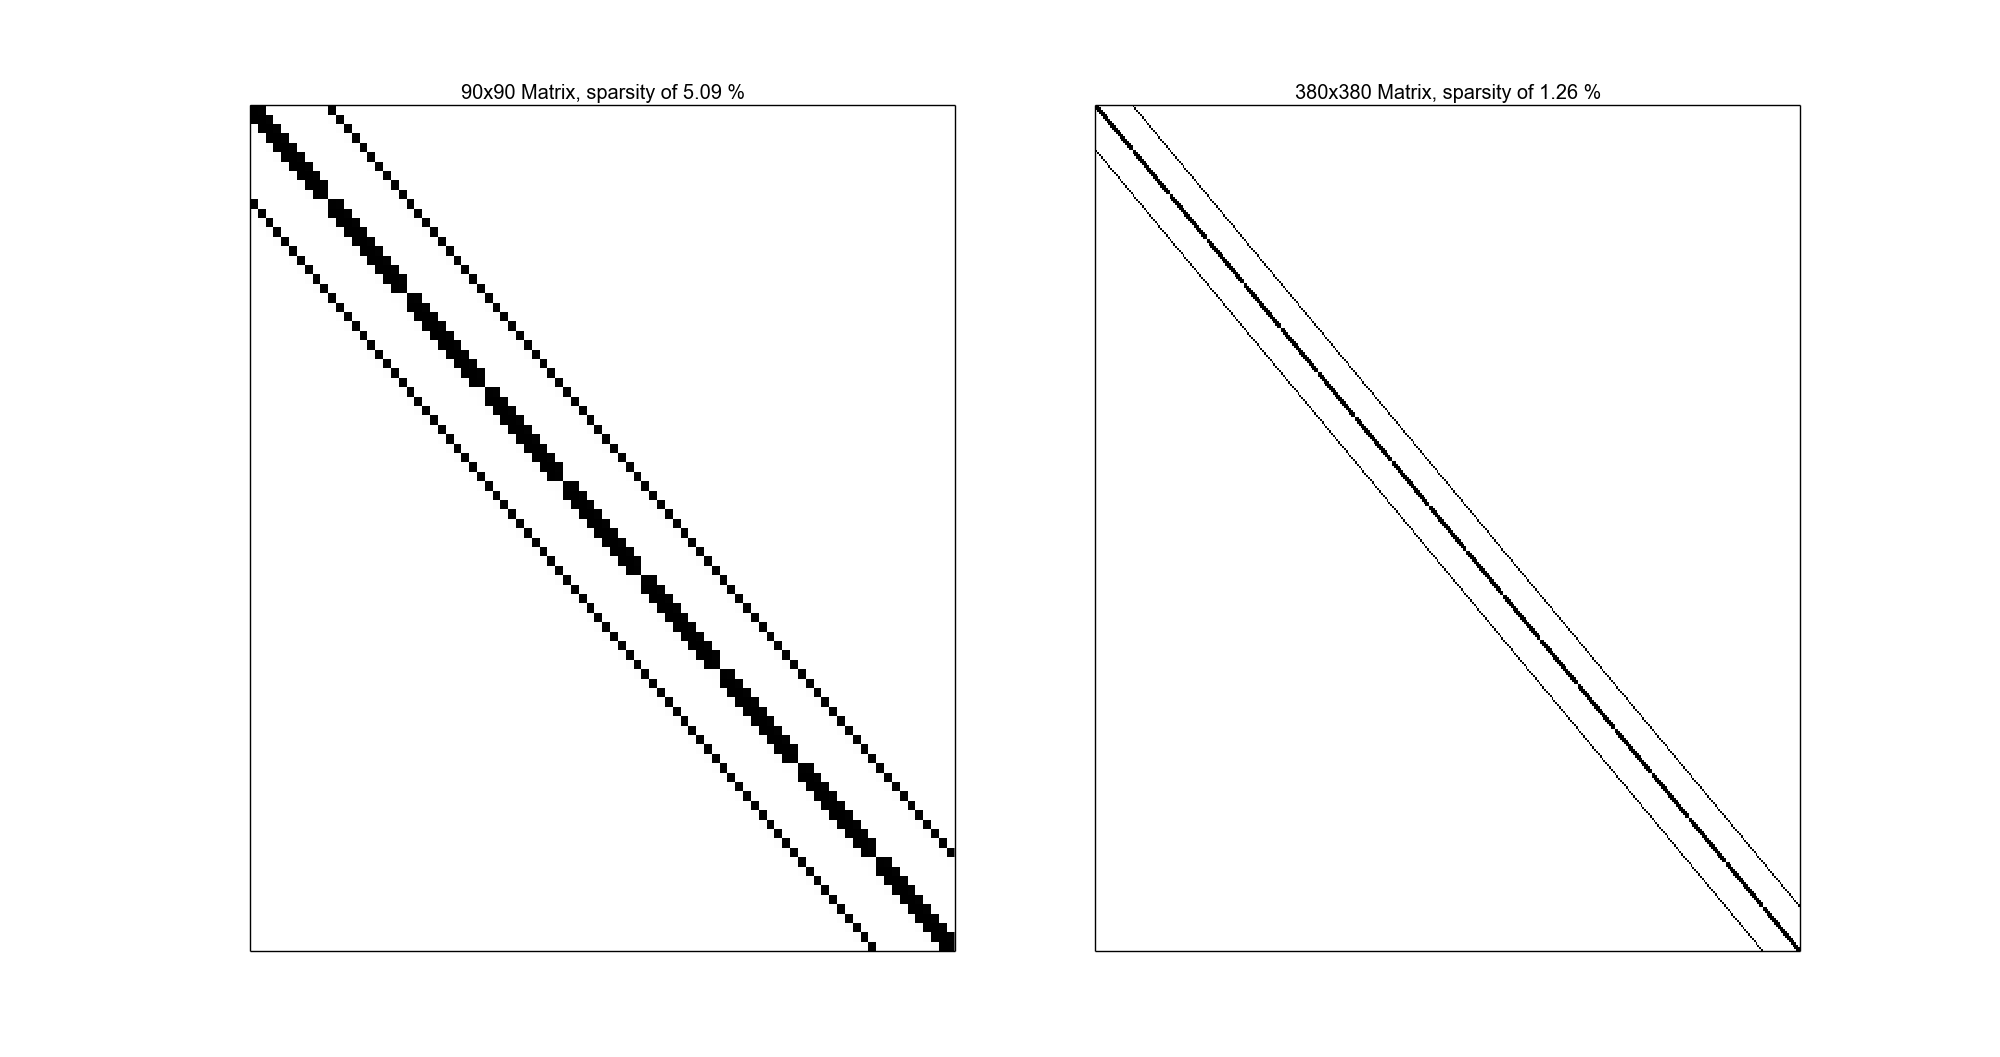
\includegraphics[scale=0.24]{sparsity.png}\caption{Example for two matrices.}
\end{center}
\end{figure}
To illustrate the fill-in induced by a LU decomposition on a sparse (tridiagonal) matrix, let's look at the LU decomposition of the matrix $A$ :
\begin{figure}[H]
\begin{center}
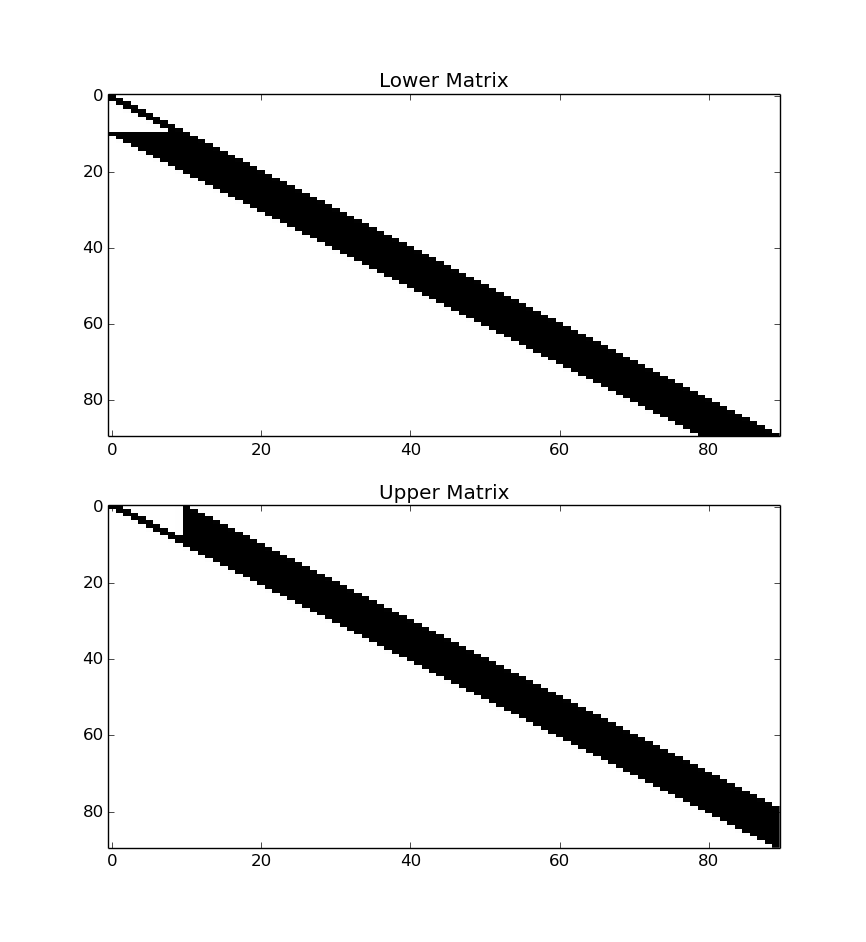
\includegraphics[scale=0.30]{LU_sparse.png}\caption{Example for two matrices.}\label{fillin}
\end{center}
\end{figure}

\subsection{Computation time,Convergence, Optimization}
Since we have a uniform mesh we can optimize the computation by not calculating every time the area of the triangles. In fact, we have by definition, triangles with the same area, only a rotation is applied.
\\
The time to fill the system is not problematic though. Here is a plot of the timed needed to fill the system compared to the number of triangles and the theoretical needed time :

\begin{figure}[H]
\begin{center}
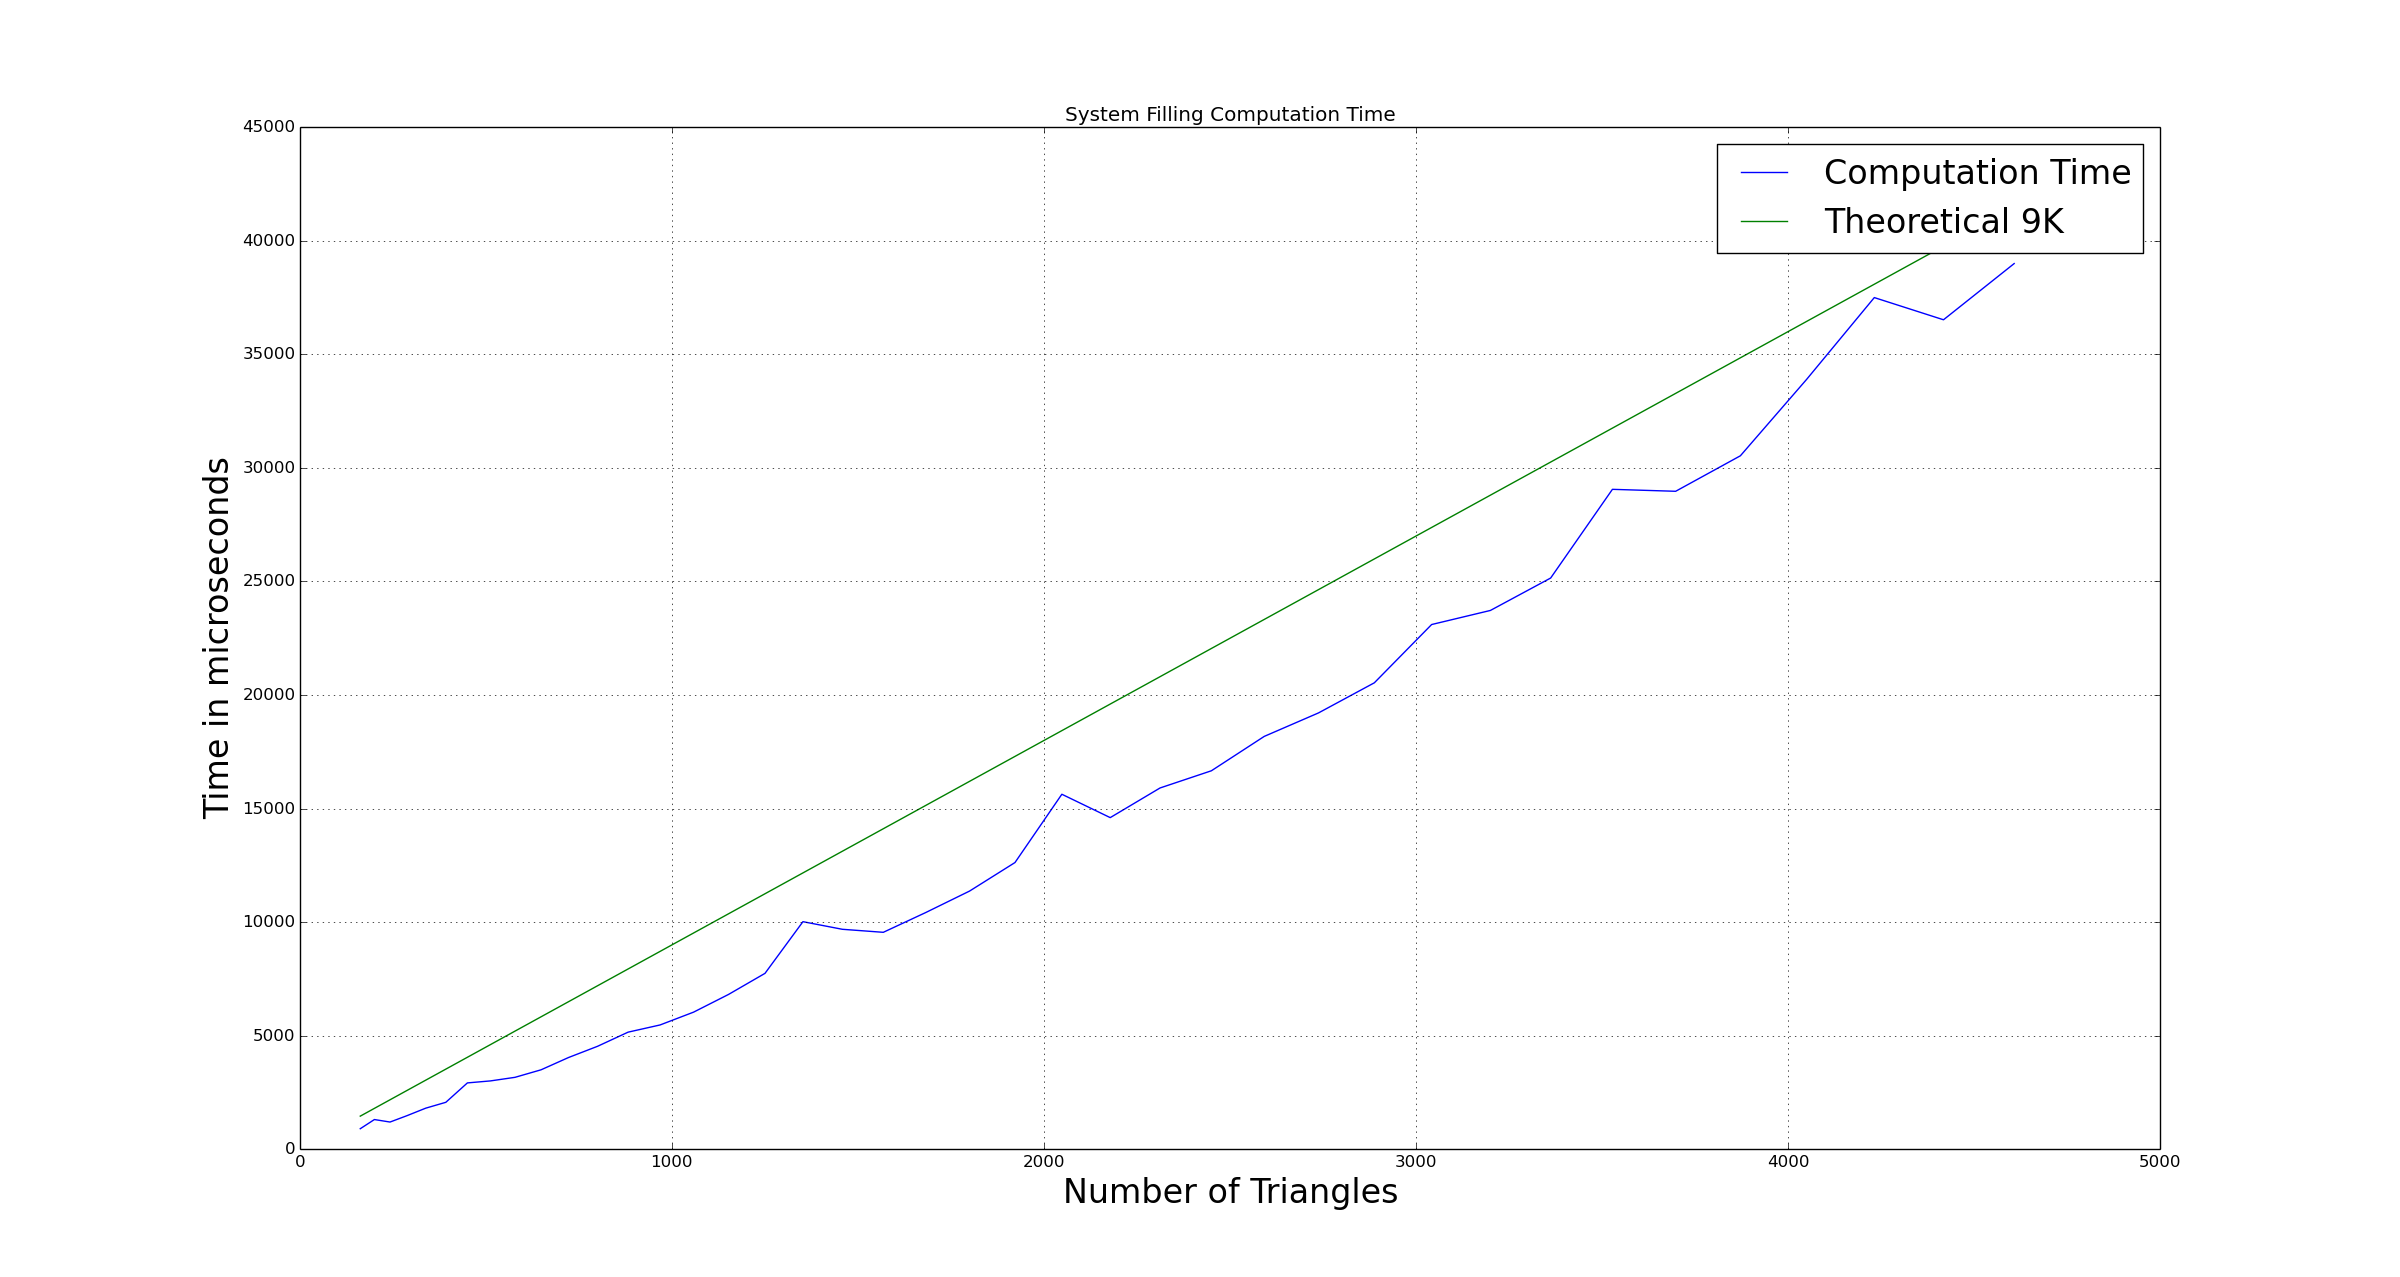
\includegraphics[scale=0.20]{filling_time.png}\caption{Time necessary to fill the system (actual time and theoretical $O(9*K)$}
\end{center}
\end{figure}

Let's now look at the required number of iterations for the solvers to converge to a solution. The error criteria taken is $1^{-9}$. Not that no preconditioning was use in this plot but this can be used with the gradient descent. however, when a preconditioning is applied to the conjugate gradient method, the convergence is not assured. This might be because the matrix $A$ which structure depends on $\alpha$ is not always positive definite.
\begin{figure}[H]
\begin{center}
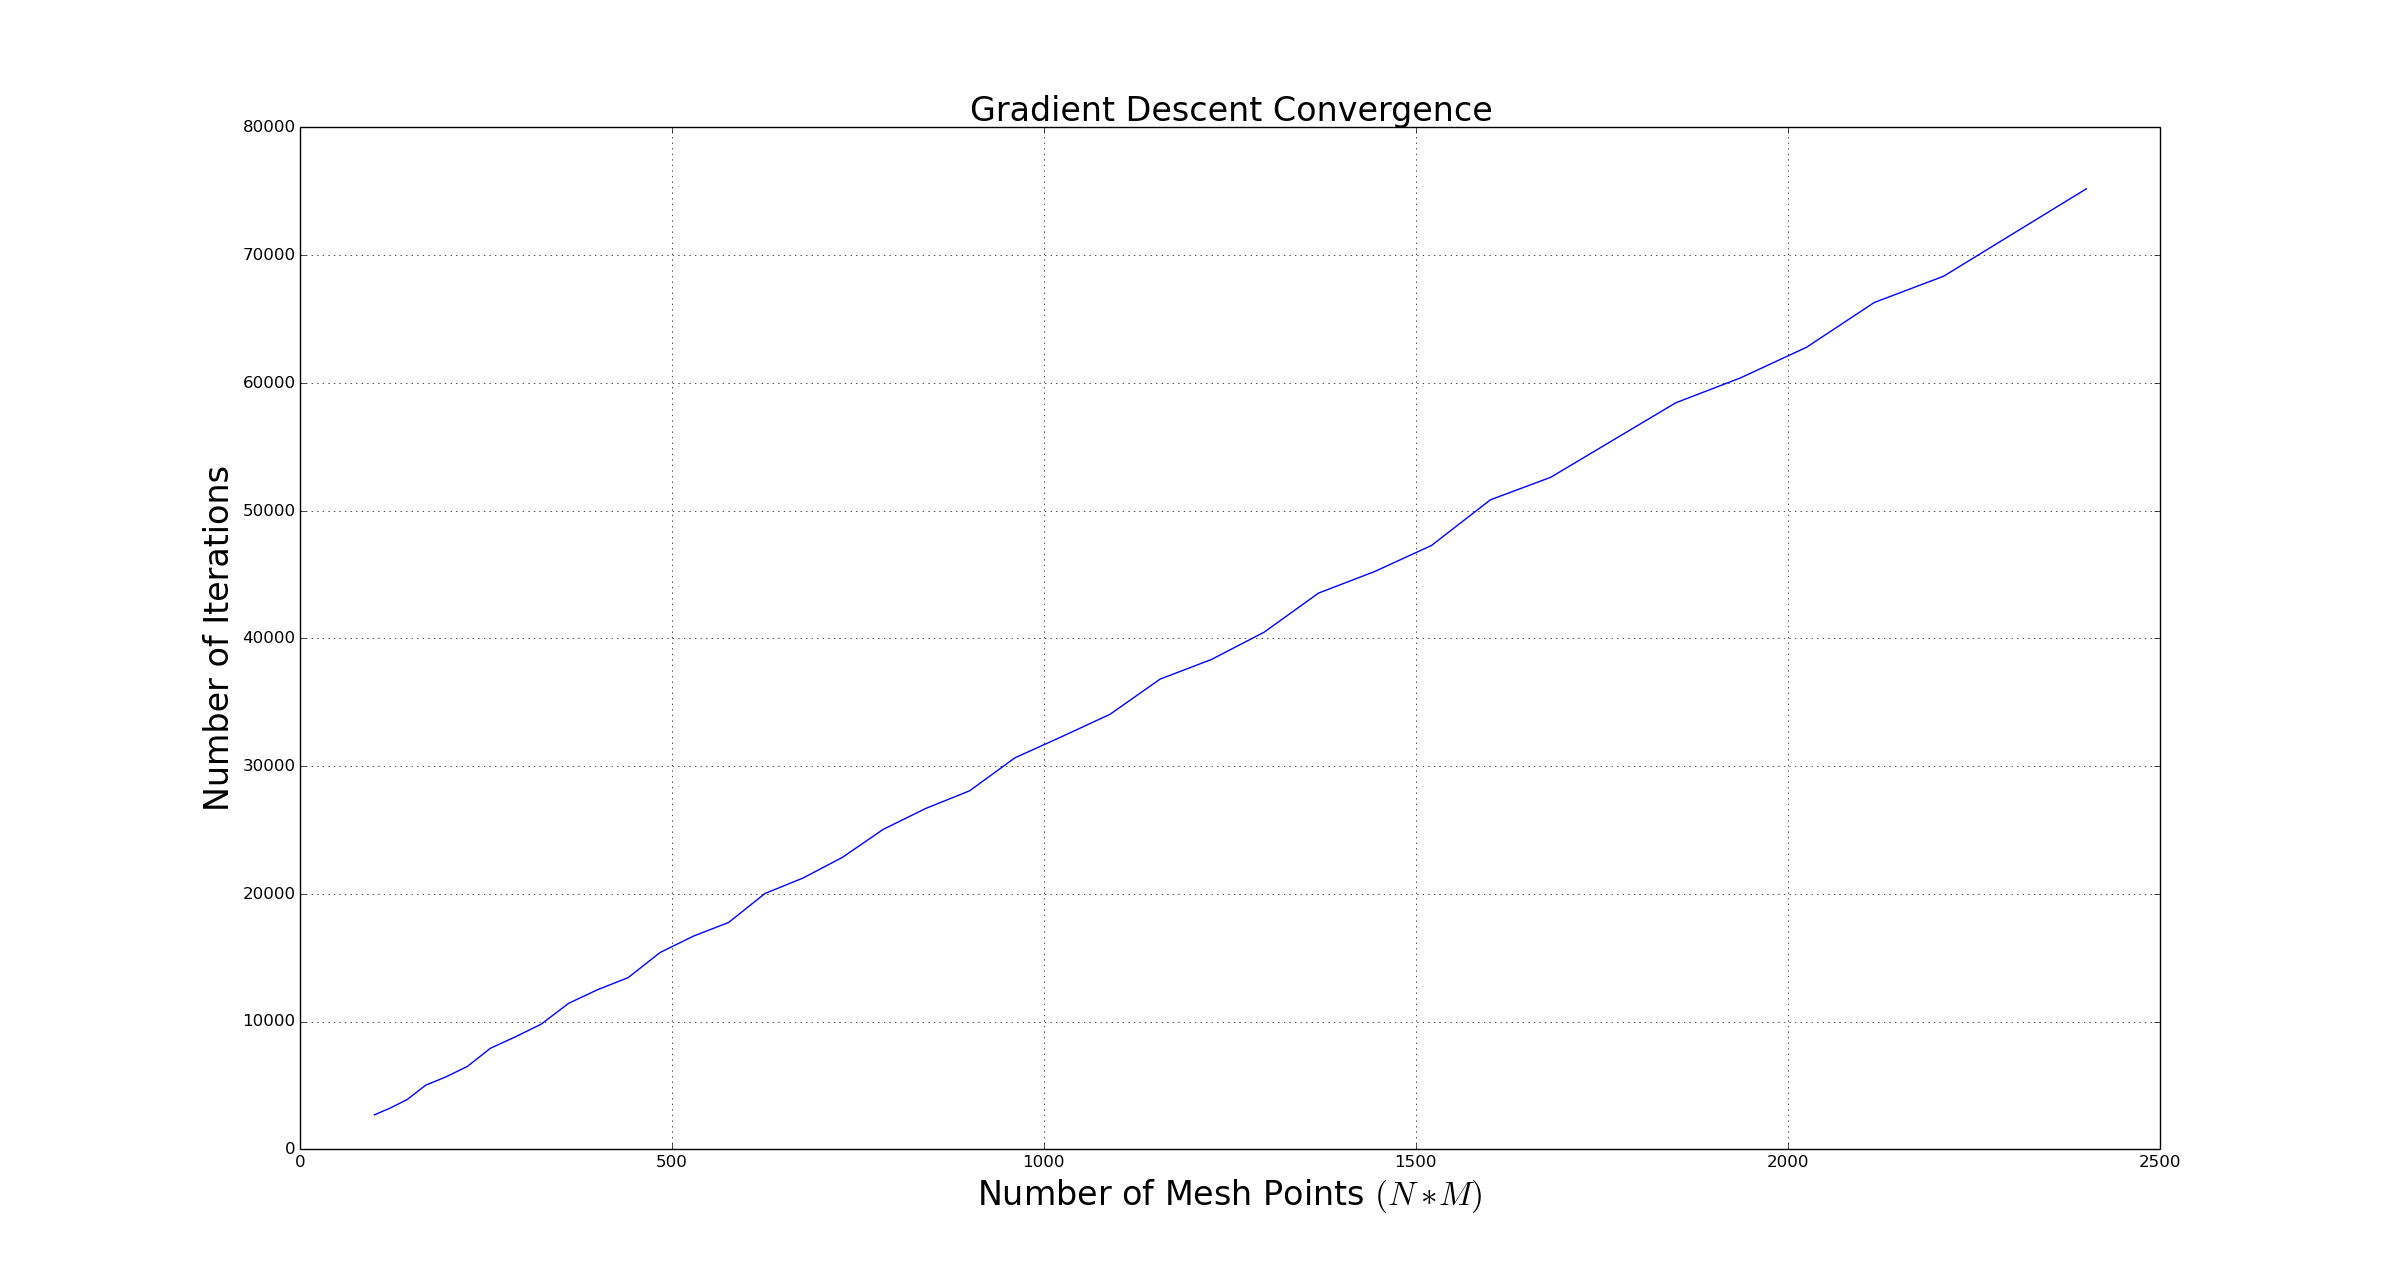
\includegraphics[scale=0.20]{GD_iter.png}\caption{Number of iterations to reach an error of $1^{-9}$ with gradient descent}
\end{center}
\end{figure}


\begin{figure}[H]
\begin{center}
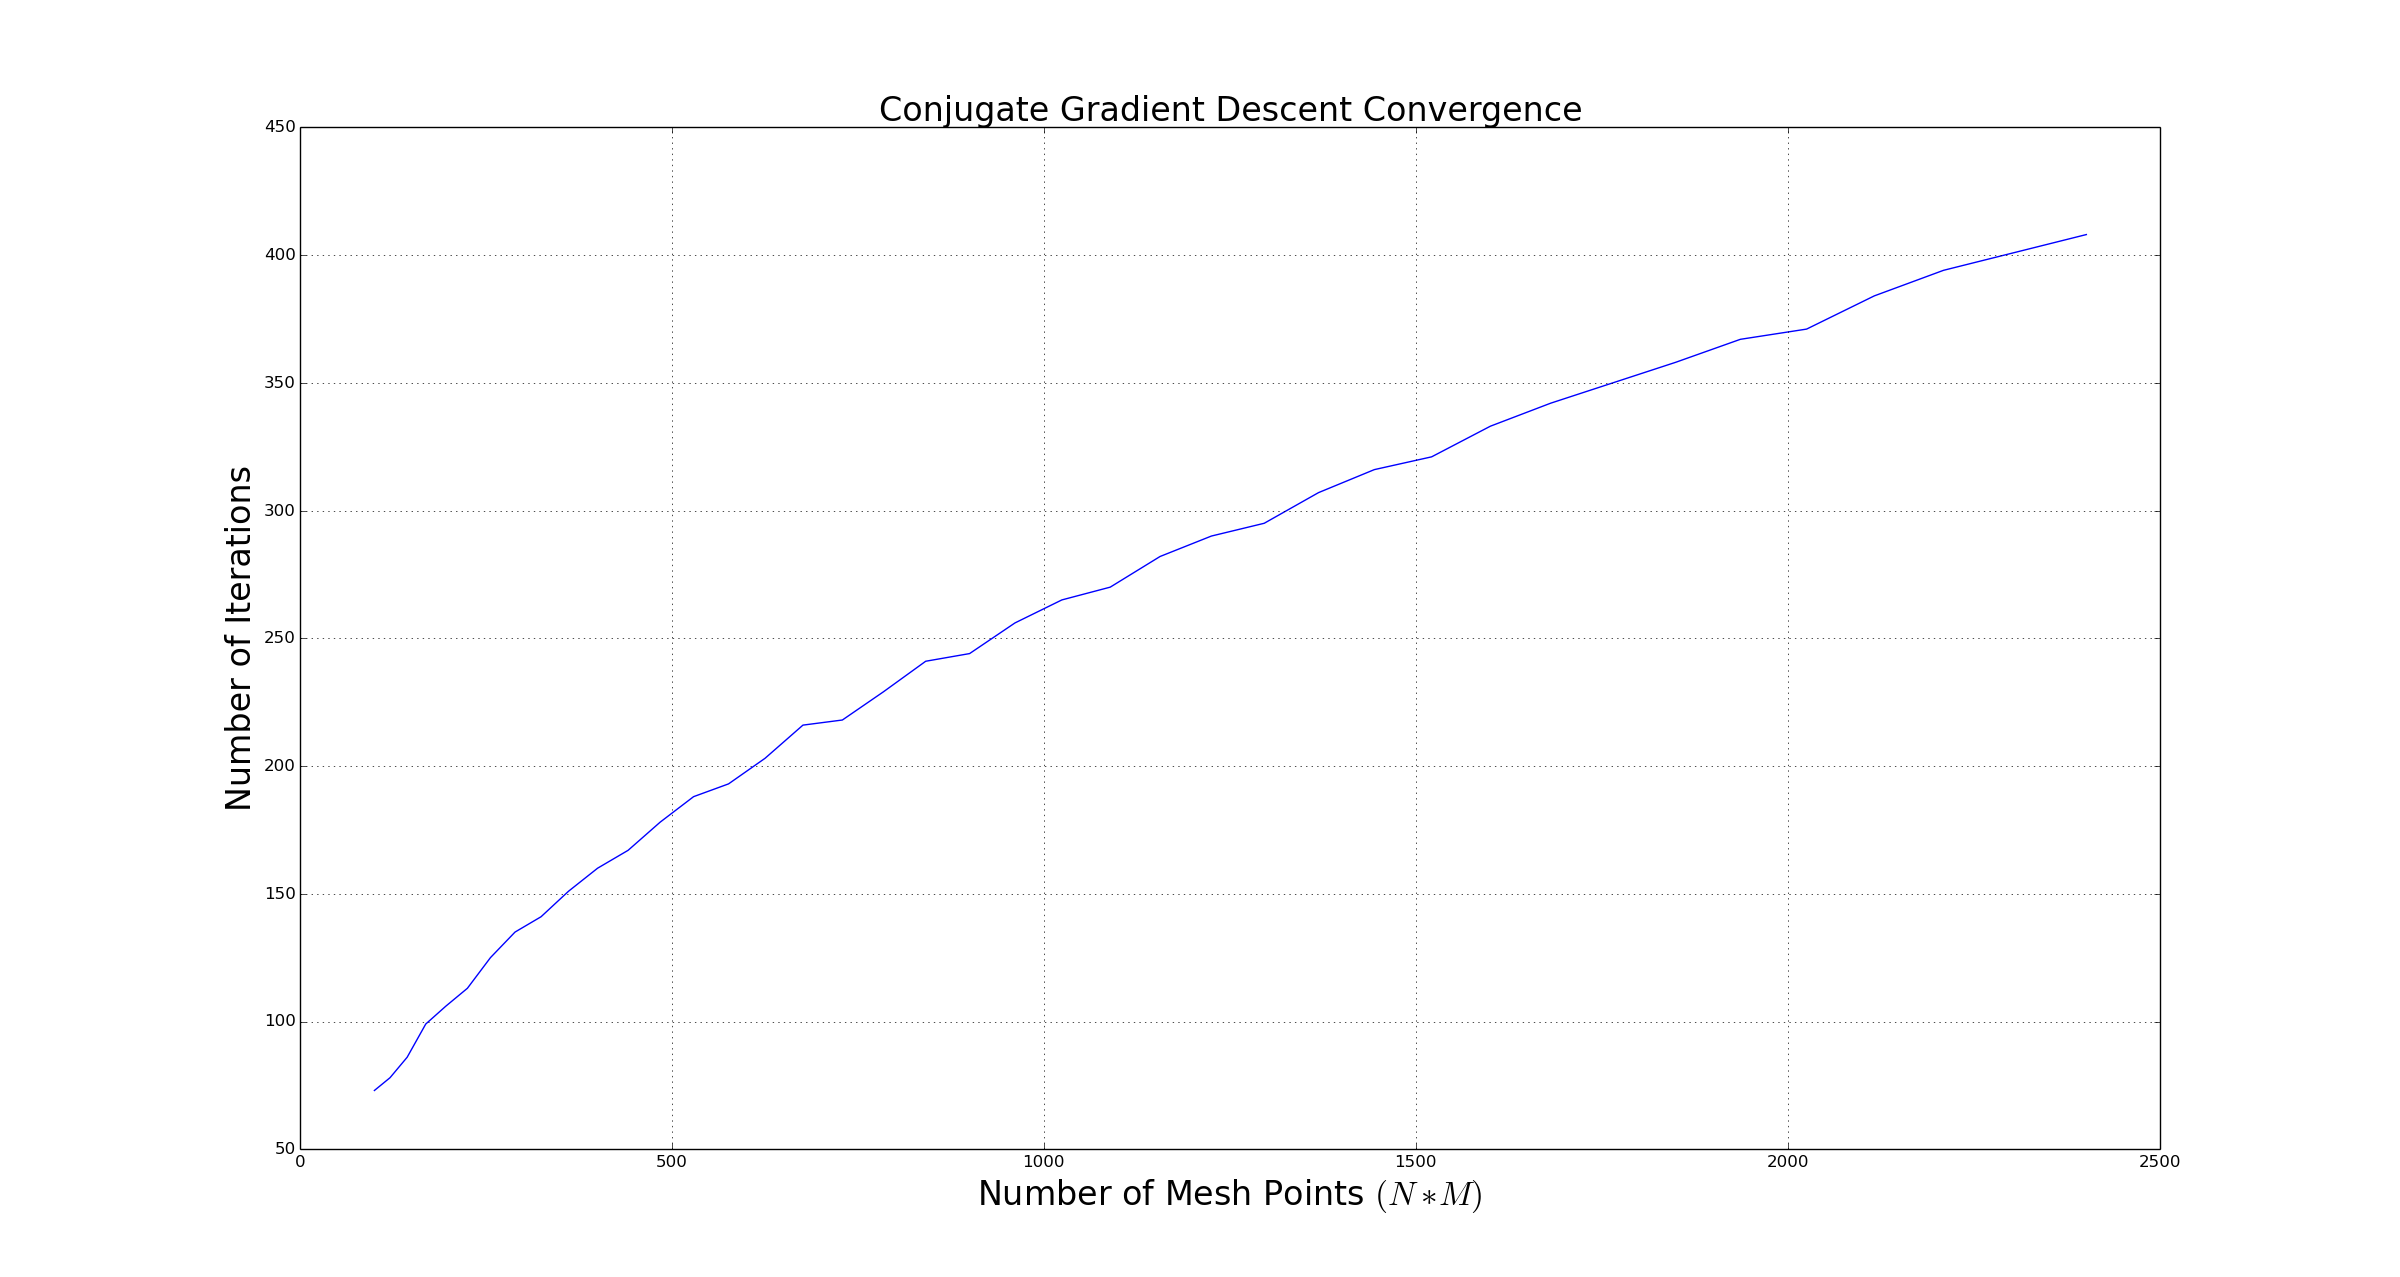
\includegraphics[scale=0.20]{CGD_iter.png}\caption{Number of iterations to reach an error of $1^{-9}$ with conjugate gradient descent}
\end{center}
\end{figure}


\chapter{Examples and GUI}
\section{GUI}
In order to facilitate the user experience, a simple Graphical Interface is provided for this project allowing quick tests. All the main parameters can be modified :
\begin{itemize}
\item the $\alpha$ function
\item the $g$ function
\item the mesh architecture
\item the solver properties
\end{itemize}
The visualization is then done in this exact interface using Qt utilities (very similar to openGL). \\
Given the mesh points $(x_i,y_i,z_i)$ for every points, the actual solution is plotted as a colored surface with a colormap (the color stands for the $z$-coordinate). For each triangle, the inside points color (needed to draw all the pixels inside the triangle) are interpolated using a bilinear interpolation according to the fact that $v_h|{T_k} \in P^1(T_k)$. This results in very nice looking visualization even with just a few mesh points as it can be seen below. \\
Let's now look at this interface and the provided utilities.
\begin{figure}[H]
\begin{center}
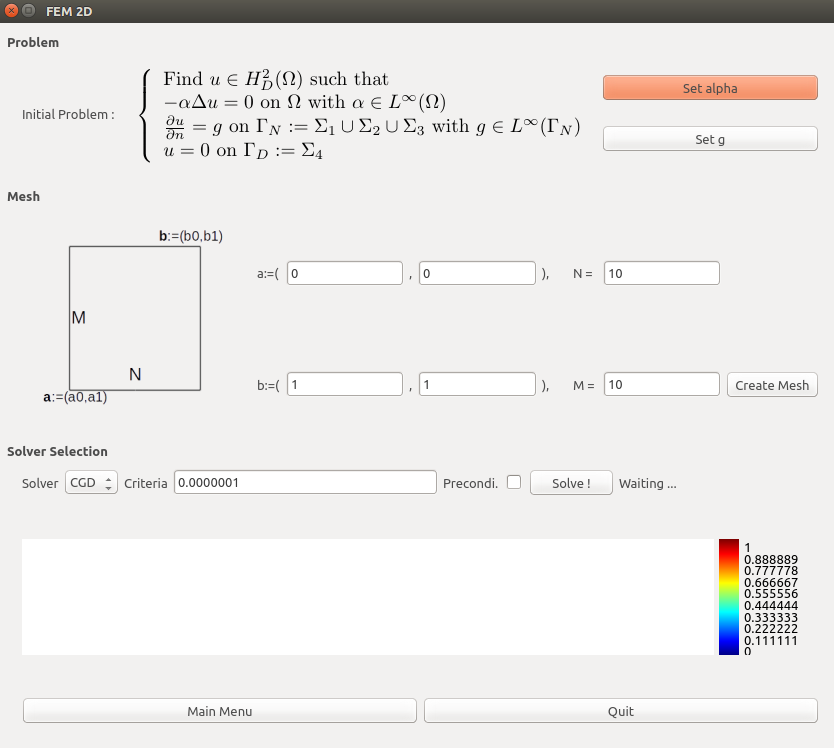
\includegraphics[scale=0.40]{fem_nude.png}\caption{Here is the main interface where every parameter can be changed and the visualization is done.}
\end{center}
\end{figure}
When clicking on the "Set alpha" button, a window appears where it is possible to set the value of $\alpha$ on every $\Omega_i$ :
\begin{figure}[H]
\begin{center}
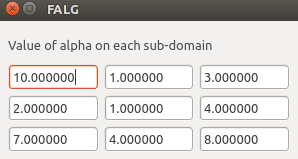
\includegraphics[scale=0.50]{set_alpha.png}\caption{Pop-up window for setting the $\alpha$ function}
\end{center}
\end{figure}
Similarly, it is possible to set the $g$ function :
\begin{figure}[H]
\begin{center}
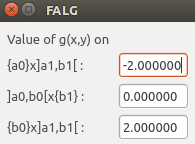
\includegraphics[scale=0.50]{set_g.png}\caption{Pop-up window for setting the $g$ function}
\end{center}
\end{figure}
Finally, the last parameter to set for the discretized problem is the number of points to use to discretize the domain. This is done by setting the parameters $N$, $M$. note that it is also possible to change the domain ($]0,1[\times ]0,1[$). When this is set, clicking on "Create Mesh" will generate the triangular mesh and draw it inside a pop up window :
\begin{figure}[H]
\begin{center}
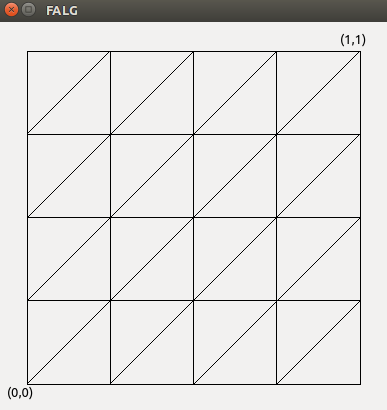
\includegraphics[scale=0.50]{mesh_5.png}\caption{Pop-up window showing the generated mesh, for a $5 
\times 5$ mesh in this case}
\end{center}
\end{figure}

\begin{figure}[H]
\begin{center}
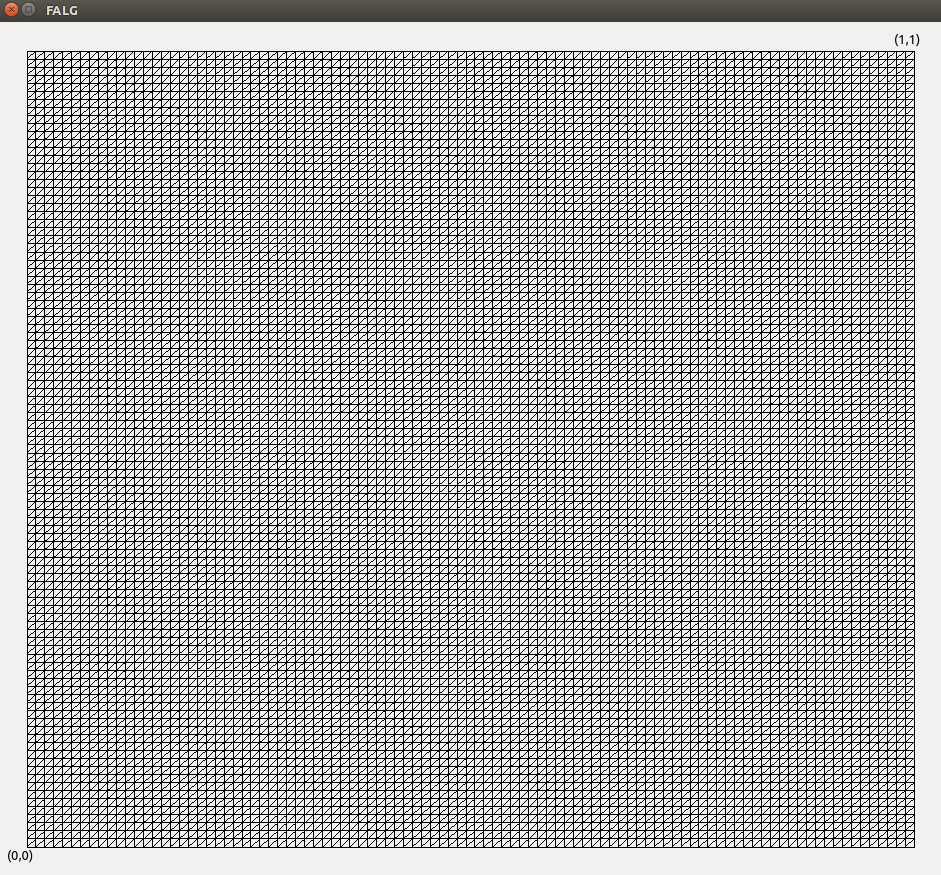
\includegraphics[scale=0.30]{mesh_100.png}\caption{Same with a much finer mesh : $100 \times 100$}
\end{center}
\end{figure}

Now setting the solver (or using the default parameters) and clicking on "Solve" will launch the solver with the generated parameters and when the approximation will be computed, the rendering process will start displaying the solution in the bottom part as shown here :
\begin{figure}[H]
\begin{center}
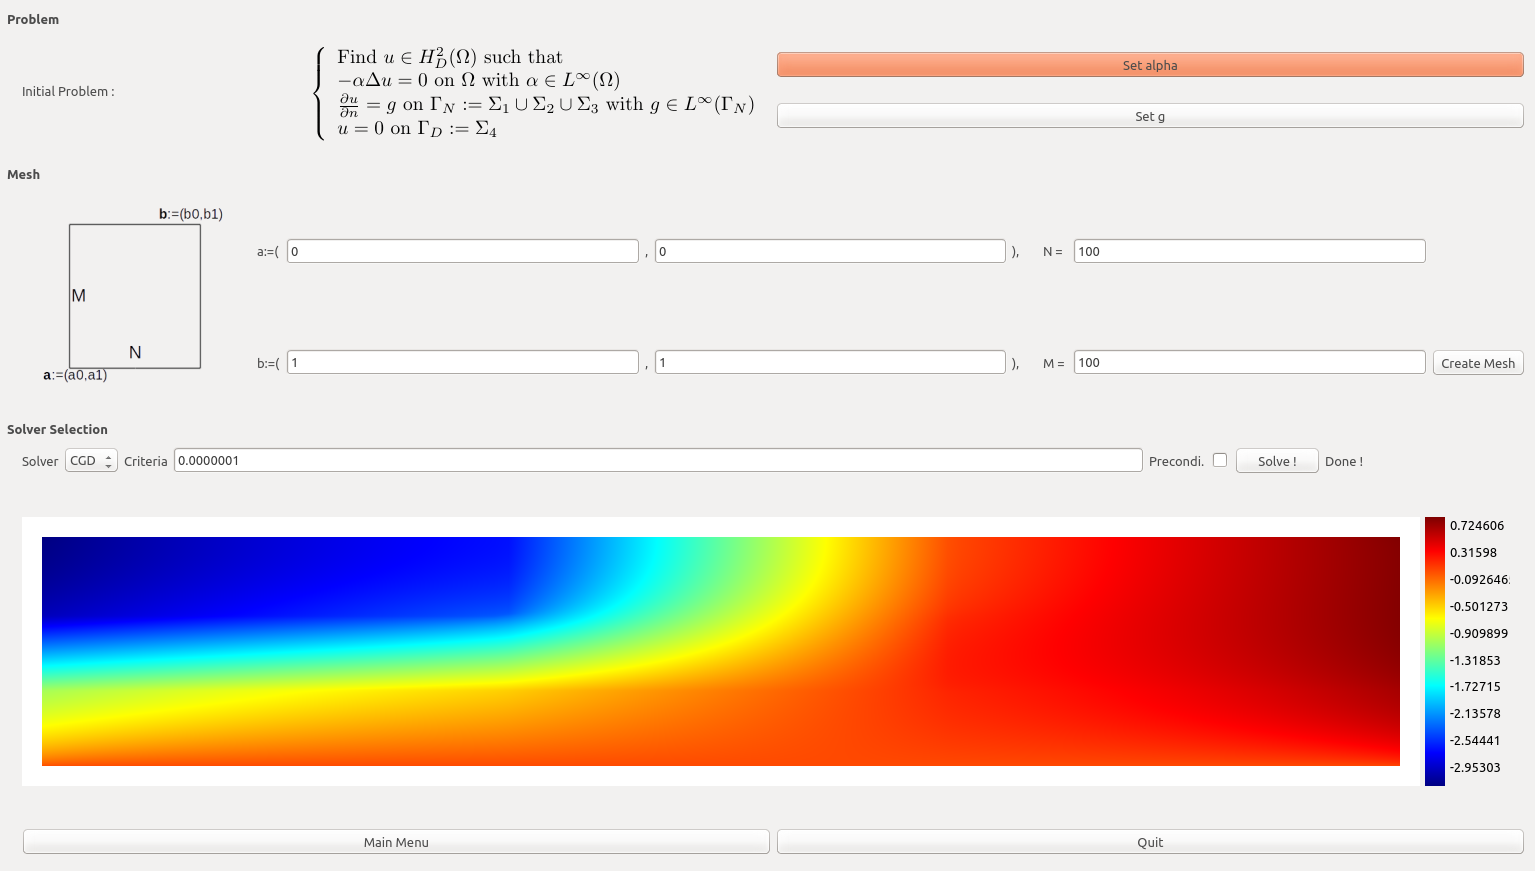
\includegraphics[scale=0.20]{fem_main_example.png}\caption{Finally the visualization of the solution after having launched the resolution process}
\end{center}
\end{figure}
\newpage
\section{Examples}
Now we will look at some more examples with other parameters, for each example are provided $\alpha$, $g$ :
\subsection{Example 1}
\begin{figure}[H]
\begin{center}
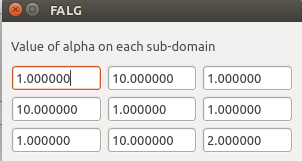
\includegraphics[scale=0.50]{example_1_alpha.png}\caption{Example 1 $\alpha$ function}
\end{center}
\end{figure}


\begin{figure}[H]
\begin{center}
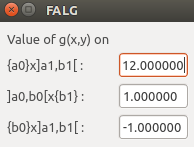
\includegraphics[scale=0.50]{example_1_g.png}\caption{Example 1 $g$ function}
\end{center}
\end{figure}


\begin{figure}[H]
\begin{center}
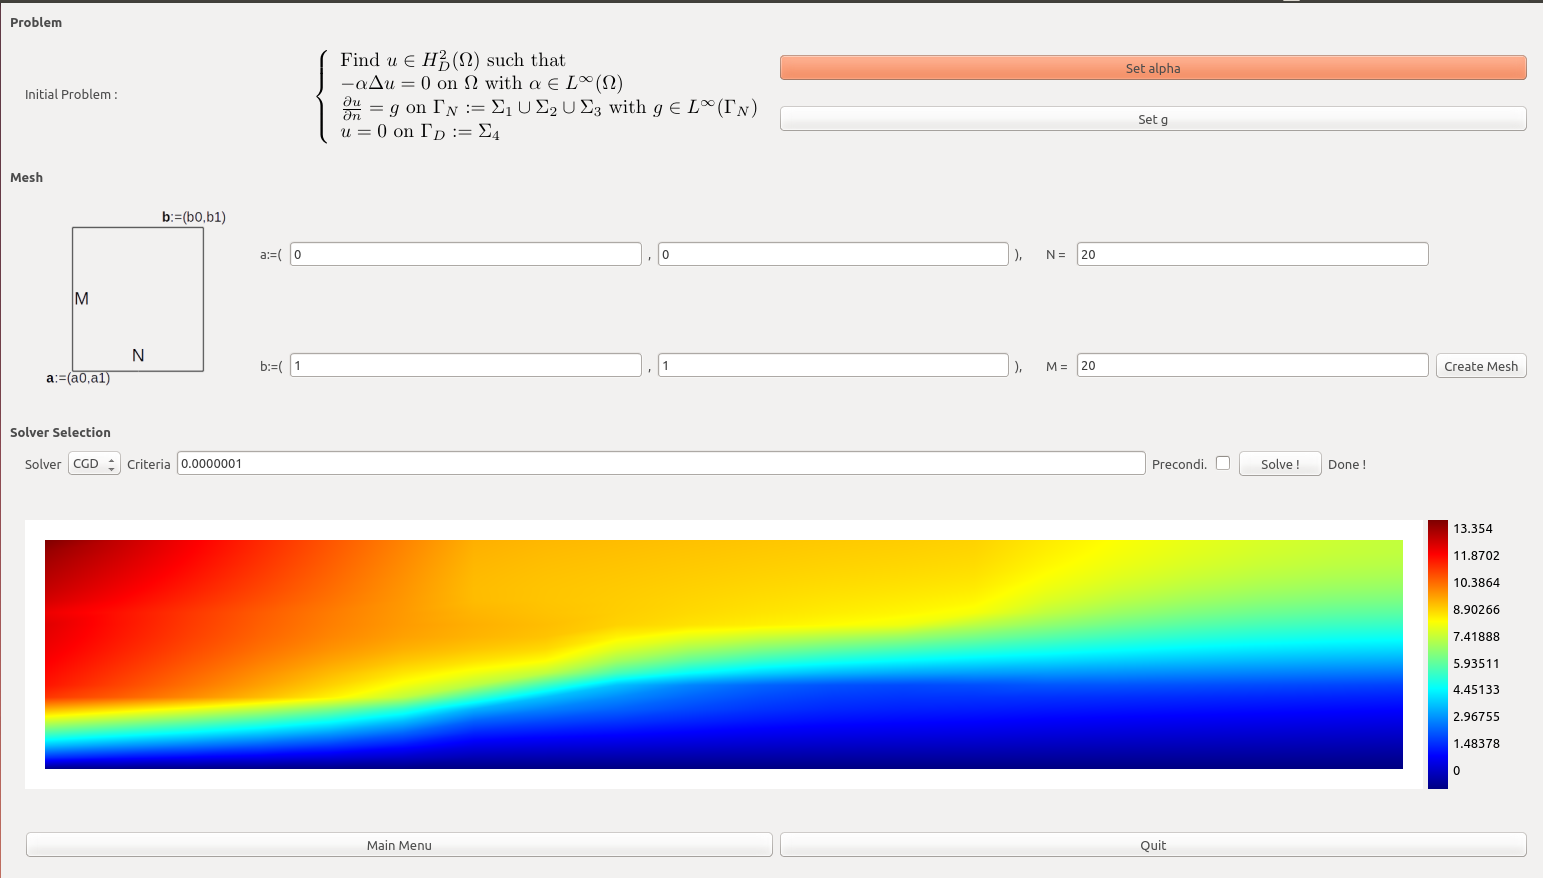
\includegraphics[scale=0.23]{example_1_solution.png}\caption{Example 1 approximated solution}
\end{center}
\end{figure}
 \newpage
\subsection{Example 2}
\begin{figure}[H]
\begin{center}
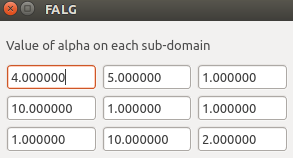
\includegraphics[scale=0.50]{example_2_alpha.png}\caption{Example 2 $\alpha$ function}
\end{center}
\end{figure}


\begin{figure}[H]
\begin{center}
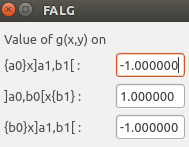
\includegraphics[scale=0.50]{example_2_g.png}\caption{Example 2 $g$ function}
\end{center}
\end{figure}


\begin{figure}[H]
\begin{center}
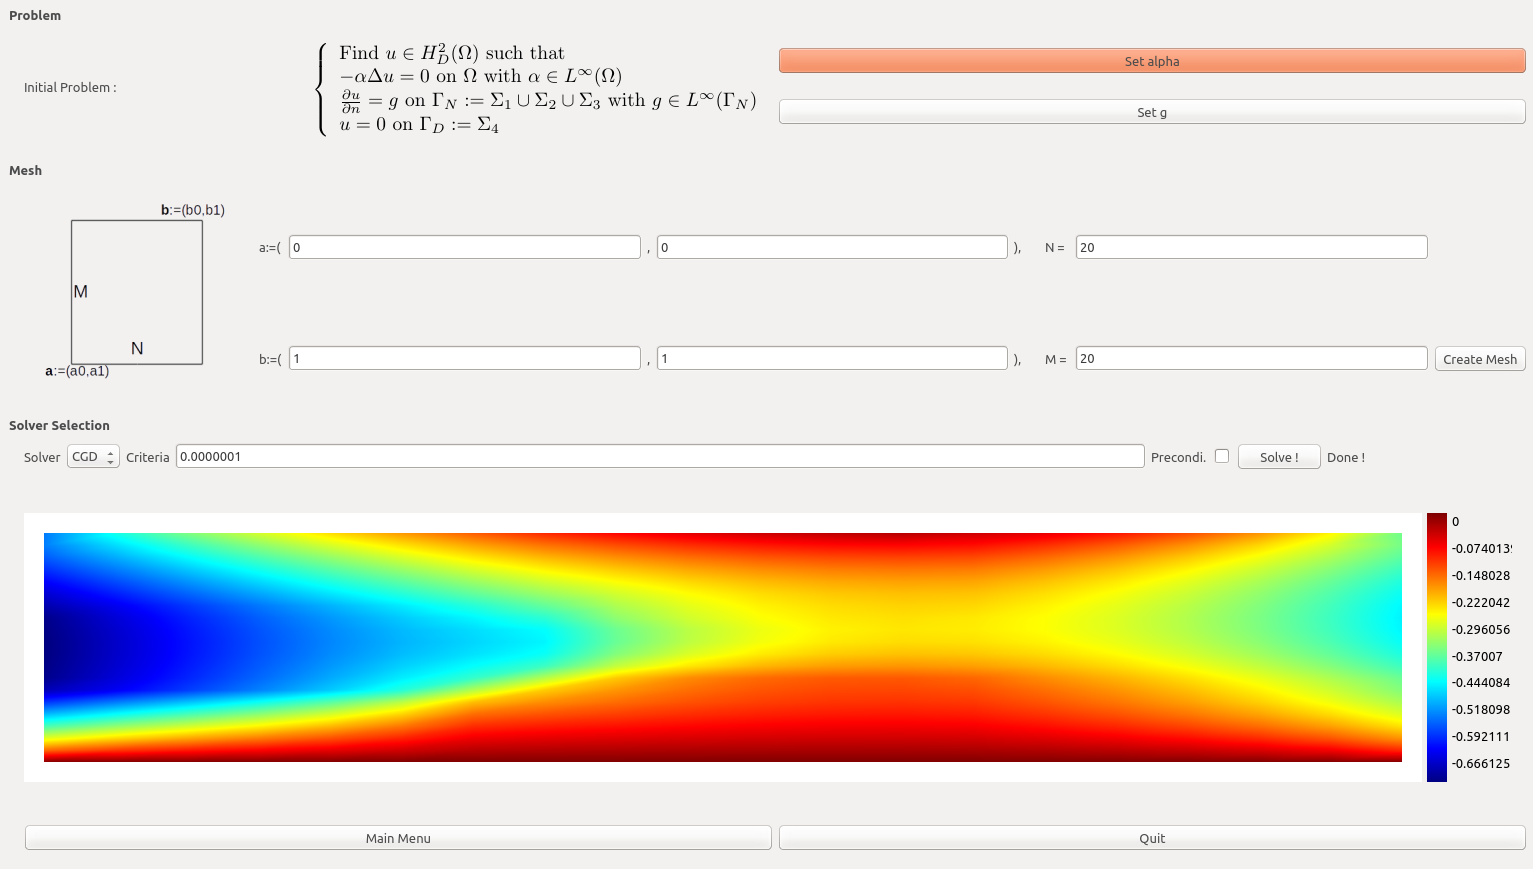
\includegraphics[scale=0.23]{example_2_solution.png}\caption{Example 2 approximated solution}
\end{center}
\end{figure}
\newpage


\chapter{Error Analysis}
\section{Considered Problem}
We will now analyse the error made by the approximation scheme by taking a reference (not exact) solution computed with a very fine mesh $150 \times 150$ and compare it with four other (less fine) meshes. We will first study the error approximation in the given interval $]0,1[ \times ]0,1[$ and then analyse the convergence rate.
\\
The studied problem is the following :


\begin{figure}[H]
\begin{center}
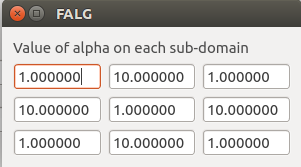
\includegraphics[scale=0.53]{reference_alpha.png}\caption{$\alpha$ function used}
\end{center}
\end{figure}


\begin{figure}[H]
\begin{center}
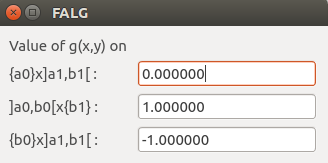
\includegraphics[scale=0.53]{reference_g.png}\caption{$g$ function used}
\end{center}
\end{figure}


\begin{figure}[H]
\begin{center}
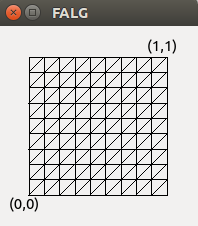
\includegraphics[scale=0.63]{reference_mesh.png}\caption{mesh used for this example (not the referenced mesh)}
\end{center}
\end{figure}

\begin{figure}[H]
\begin{center}
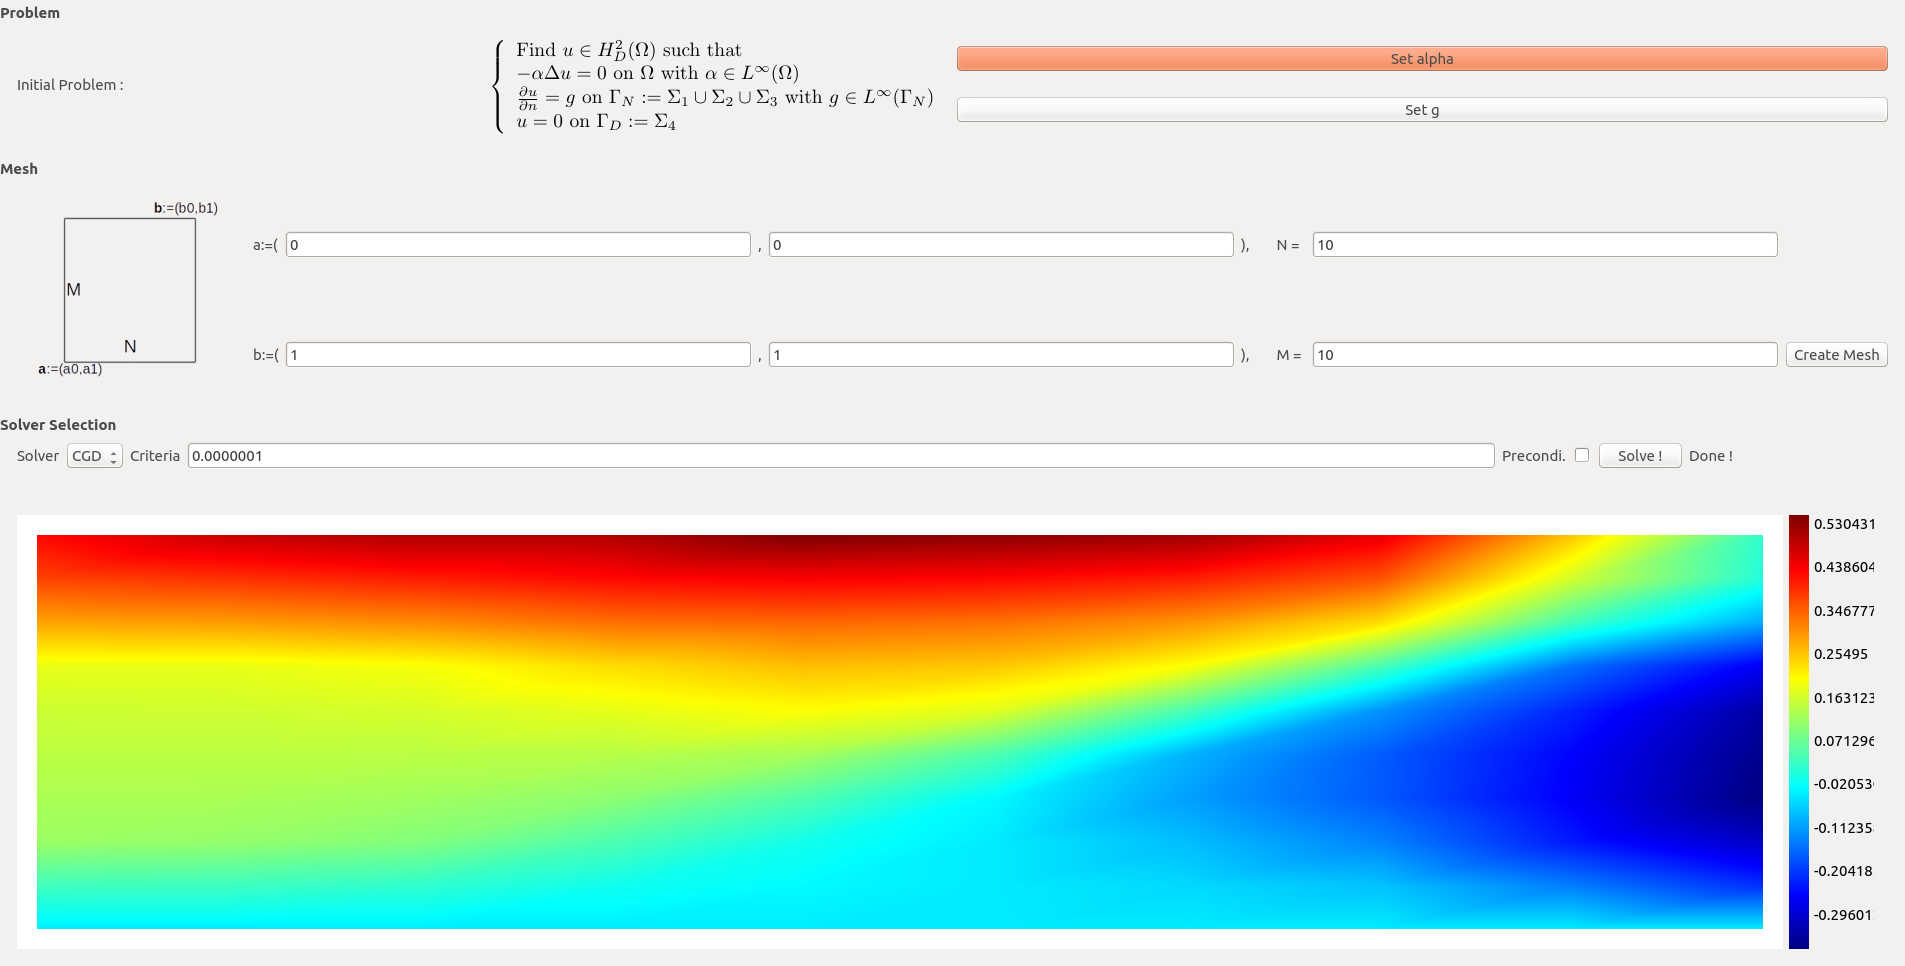
\includegraphics[scale=0.20]{reference_sol.png}\caption{Solution example with this mesh}
\end{center}
\end{figure}


\section{Analysis}
The four considered meshes that will be used against the $150\times 150$ mesh are : 
\begin{itemize}
\item $ 9\times 9:=M_1$
\item $12 \times 12:=M_2$
\item $24\times  24:=M_3$
\item $36 \times 36:=M_4$
\end{itemize}
Firstly, we will look at the error made for each mesh with a global colormap in order to emphasize the error reduction when the mesh gets smaller.\\


\begin{figure}[H]
\begin{center}
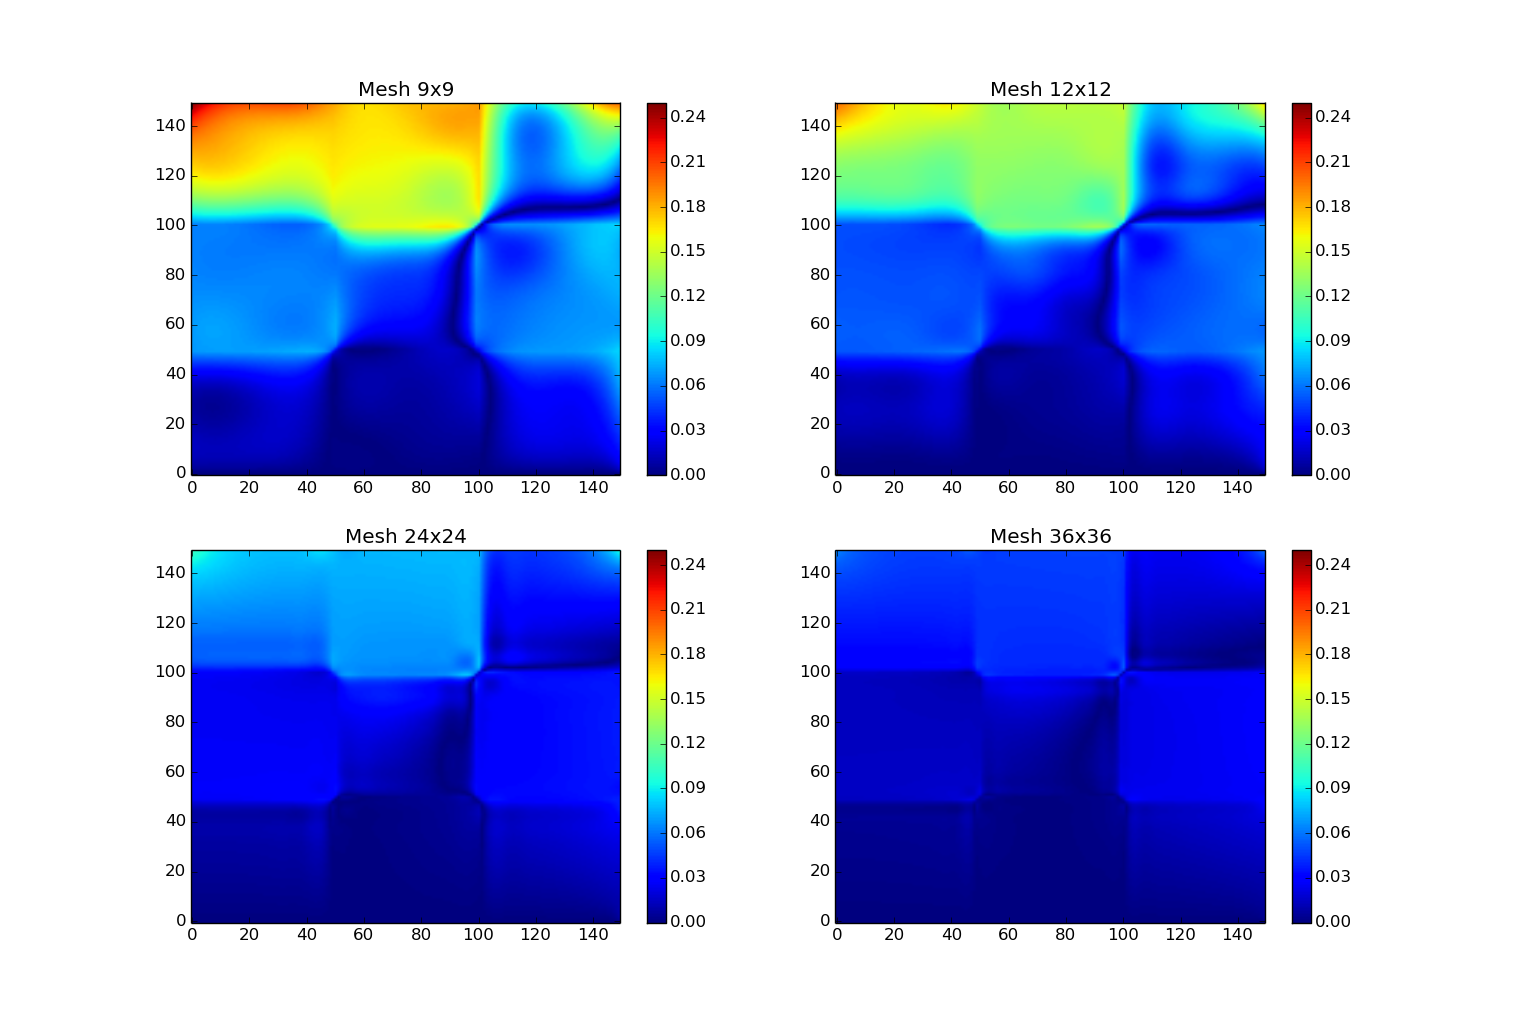
\includegraphics[scale=0.37]{errorvsnorm.png}\caption{Reference 150x150 mesh, with global colormap}
\end{center}
\end{figure}
In this case, each subplot represents $|M_{ref}-M_i|$ but the key here is that the colors (corresponding to the error made on each mesh point) is using the biggest error of $M_1$ and the smallest error of $M_4$ as a range for the colors.\\
Thus it is clear that the error is reduced by taking a finer mesh.\\
Note that once again this result has been computed using bilinear interpolation when needed but this is exact by the definition of $V_h$.
\\
The problem is that we can see the evolution of the error through the different meshes but not really the error repartition for each mesh, thus, here is the same plot but with each subplot having an independent error range and coloration :
\begin{figure}[H]
\begin{center}
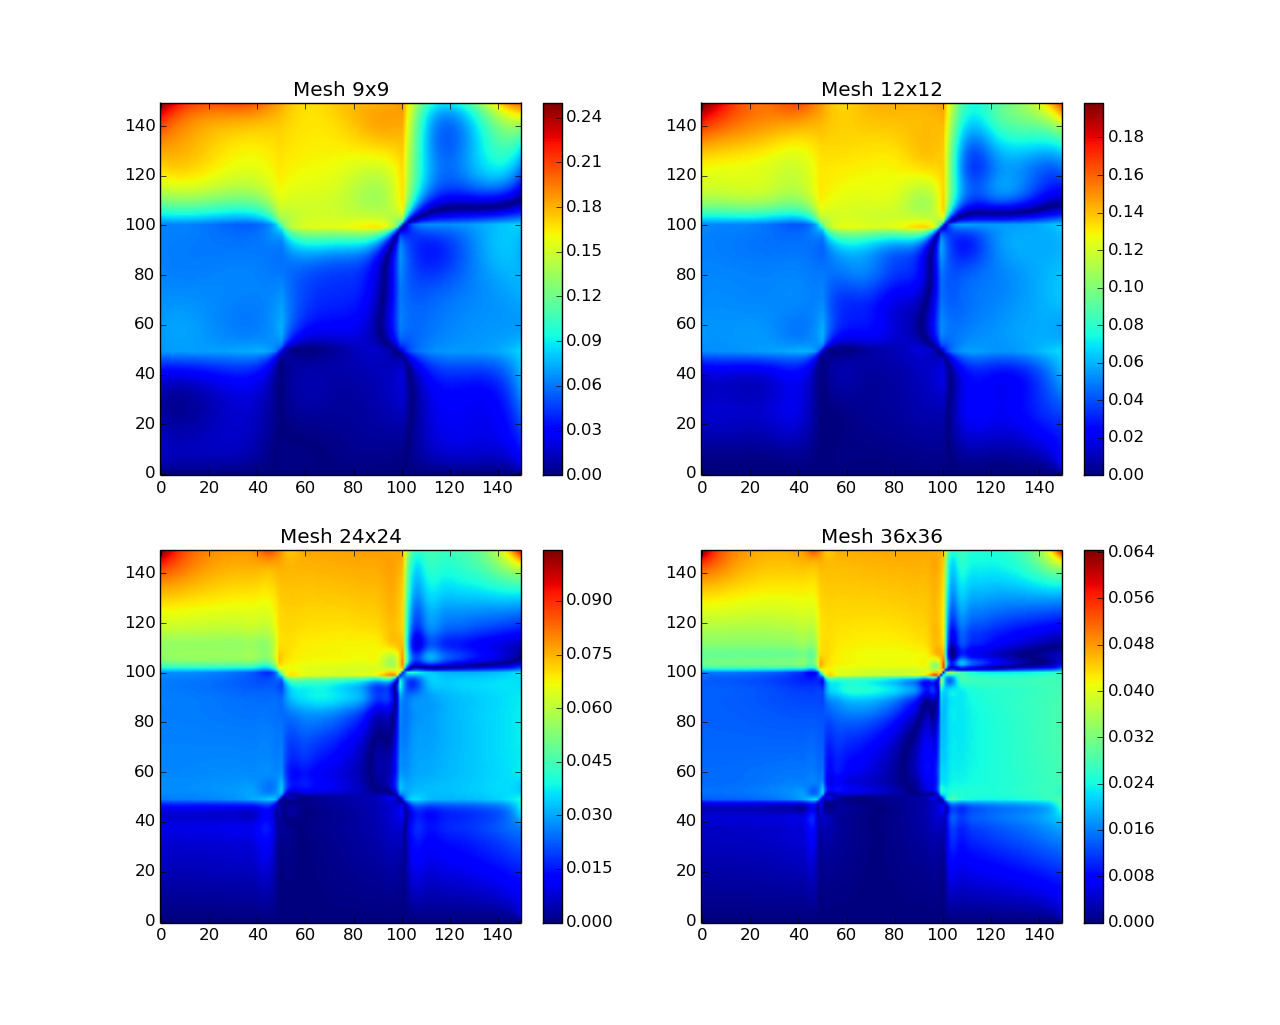
\includegraphics[scale=0.42]{errorvs.png}\caption{Reference 150x150 mesh, with individual colormap}
\end{center}
\end{figure}
Now we can clearly see that the middle-top sub-domain $\Omega_i$ is always problematic whatever the mesh we use. In addition, the top left corner is where the error is the biggest. This analysis could be an indicator that in the sub-domain in question (middle-top) we should use a finer mesh and maybe in the top corners too.
\\
Let's now see the error ($||.||_{H^1}$) made by these approximations compared to the reference one :

\begin{figure}[H]
\begin{center}
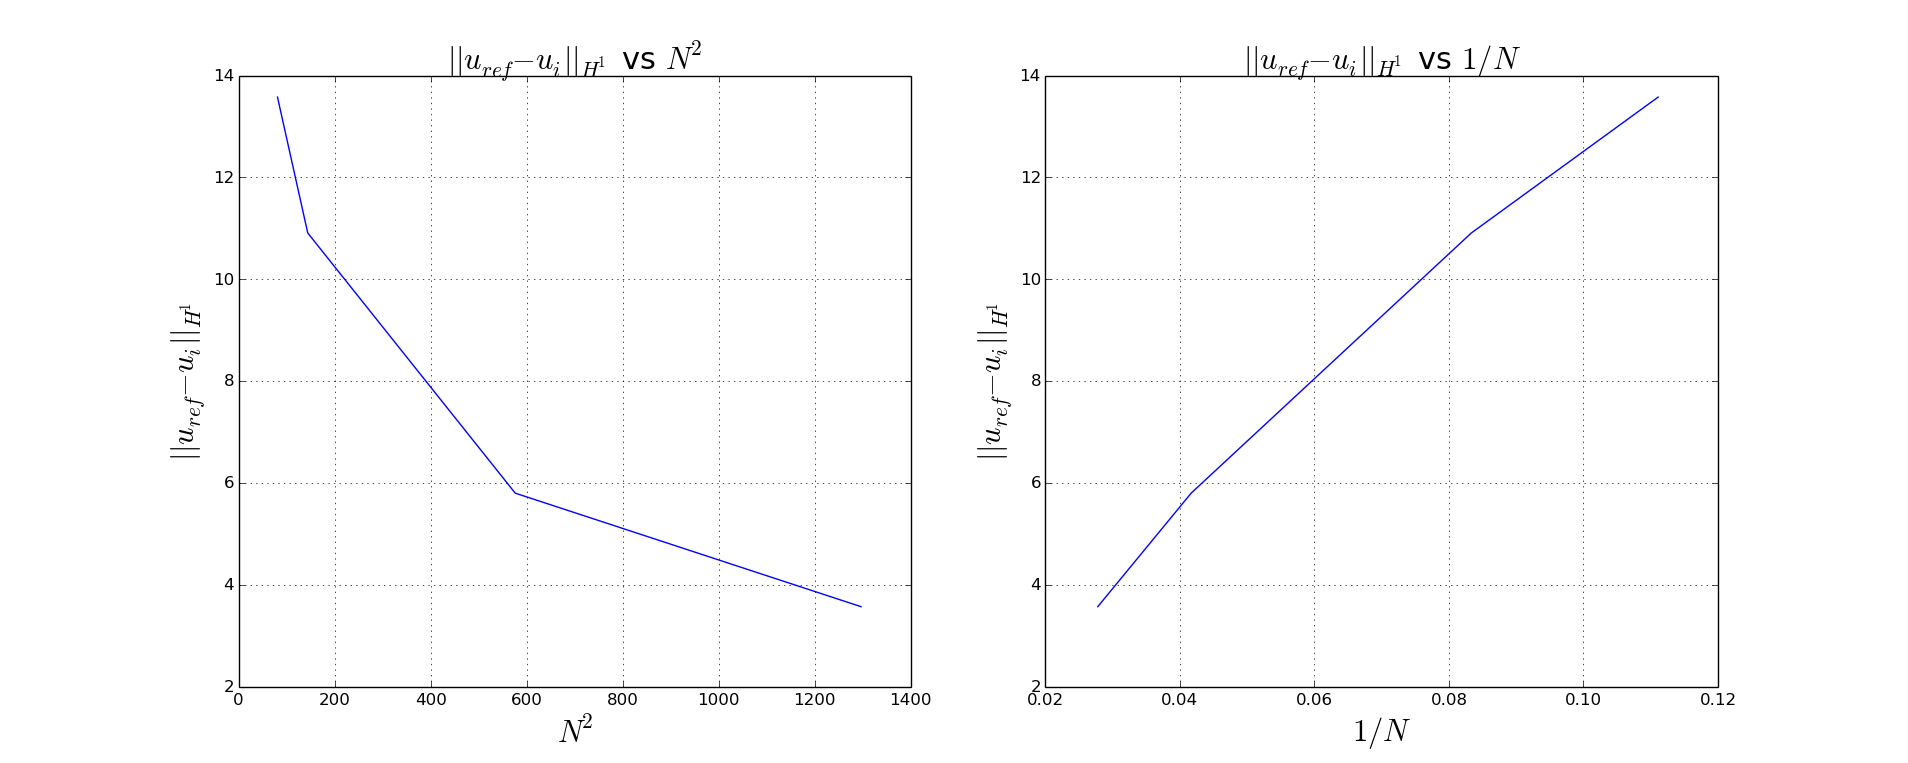
\includegraphics[scale=0.25]{error_h.png}\caption{Reference 150x150 mesh showing the $O(h)$}
\end{center}
\end{figure}
When we plot the error versus $1/N$ we clearly see the error which is of order $h$ with $h$ being the mesh steps. This is in fact what was expected when using a $P^1$ Lagrange basis. 
\section{Conclusion}


The presented challenge is really a unique experience for testing algorithms around bioacoustic classification. This task contains all the main difficulties and problems encountered in a real life problem while involving a huge dataset. 
\\
We have seen that the scattering transform provides a wonderful new data representation but it is not yet easy to know how to extract features from its coefficients. We obviously didn't try every possible algorithm but the idea of thresholding/combination in the $\lambda_2$ dimension seems to be interesting. The key part is to be able to capture feature with a time-invariant algorithm in term of the position of the feature in a signal, but, we need to keep a "time" component to analyse frequencies evolution inside the features.
\\

Given the massive dataset it has also been a unique experience to learn ways and methods to deal with computational limitations and the challenge deadline.
more importantly, this has helped to deeply understand the scattering network and the pre-processing part in general when trying to apply machine learning algorithms for a given task.


\bibliographystyle{plain}
\bibliography{ref2}
\nocite{*}

\end{document}
